\chapter{Montagem eletrônica}
%\section{Lista de Materiais}

%\begin{table}[H]
%\centering
%\begin{tabular}{|m{1.8cm} |m{9.2cm}|m{4cm}|}
%\hline
%\begin{center}Quantidade\end{center} & \begin{center}Componente\end{center} &\begin{center} Part Number\end{center} \\\hline
 %03&Lora Esp32 Sx1278 Com Display  Oled Wifi bluetooth 915mhz& Sx1278 \\\hline
 
%03 &  Conversor DC-DC Step Down-LM2596 (12~5V)
%& LM2596 \\\hline
  
%01& Módulo Gps  Gy-gps6m v2 & GPS NEO6M \\\hline
   
%03&LConector Borne KRE 2 Vias & KRE Kf301 \\\hline

%01&Sensor De Pressão e Temperatura BMP 280 & BST-BMP280-DS001-11 \\\hline

%01&Módulo Cartão de Memória MICRO SD CARD & B01IPCAP72 \\\hline

%01& Driver Motor Ponte H L298n & L298 \\\hline

%01&Módulo Conversor Nível Lógico 5V/3.3V -Bidirecional&  MOD-CXI2C \\\hline

%02& Sensor de Peso 50Kg Célula de Carga & SEN-10245\\\hline

%01&Módulo Hx711 Célula De Carga Balança 24 Bits & HX711 \\\hline

%14& porca de bronze espaçador hexagonal M5 X 12mm & -  \\\hline

%02 &  Módulo Relé 5V 2 Canais &   SRD-05VDC-SL-C \\\hline

%03 & Conector Jack J4 DC Fêmea &  Jack Fêmea  \\\hline

%02 & Conector Adaptador Plug P4 Macho com Borne &  P4 Macho F0503 \\\hline

%01 & Micro Usb V8 Macho & J5415\\\hline

%01 & Plug Hdmi Macho & Hdmi Macho \\\hline

%01 & NVIDIA Jetson Nano Developer Kit  & 945-13450-0000-100 \\\hline

%01 &Placa controladora   & PCB800099-V.9  \\\hline

%01 & Display LCD 9 polegadas  & Lcd 9 Polegadas TMOEC \\\hline

%01 & Mini  Teclado  slim  com  Touchpad & -  \\\hline

%01 & PCI- Base & -  \\\hline
%01 & PCI- Foguete & -  \\\hline
%01 & PCI- Maleta & -  \\\hline

%\end{tabular}
%\caption{Lista de componentes}
%\end{table}

\section{Ferramentas}

\par Para a soldagem dos componentes eletrônicos nas PCIs (Placas de Circuito Impresso), conexões dos fios com os módulos necessários e fixação da PCI na case de proteção ou outro local, é necessário o uso das seguintes ferramentas e acessórios:

\begin{itemize}
    \item Ferro de Solda ou Estação de Solda (15W-40W)
    \item Solda Estanho em fio 1mm
    \item Esponja metálica ou esponja convencional para limpeza da ponta de solda
    \item Lupa com suporte e pinça, para apoio e manuseio da PCI
    \item Sugador de solda
    \item Chave de fenda/phillips
    \item Alicate de corte pequeno
    \item Alicate de desencapar ou estilete
    \item Multímetro
\end{itemize}

\begin{center}
ATENÇÃO
\begin{figure}[H]
 \centering
 
\includegraphics[scale = 0.1]{Figuras/atenção.png}
\end{figure}
\end{center}

\par Os ferros de solda aquecem a temperaturas superiores a 400ºC. Usar um suporte para ferro de solda de boa qualidade é fundamental para não se acidentar e sofrer com queimaduras. Além disso, certifique-se de trabalhar em uma área bem ventilada ou use um extrator de fumaça ou exaustor de fumaça. Os vapores do fluxo são tóxicos. Leia atentamente as instruções deste manual. Ao soldar, utilize Equipamentos de Proteção Individual (EPIs), tais como, óculos de segurança e luvas de segurança. Mantenha todo o cabelo, roupas folgadas e joias protegidos e fora do caminho de suas ferramentas. Se a solda que você estiver usando contiver chumbo, lave as mãos após concluir o trabalho.


\subsection{Boas práticas}

\subsection{Manuseio da PCB e componentes eletrônicos}
\PAR É de bom grado ter alguns cuidados ao montar e manter em boas condições as placas de circuito impresso-PCI que estão sujeito a vários fatores de risco como:
\begin{itemize}
\item \textbf{Mecânicos:}
\begin{itemize}
\item Vibrações
\item flexões nas PCI 
\item choques mecânicos
\end{itemize}
\end{itemize}

\begin{itemize}
\item \textbf{Ambientais:}
\begin{itemize}
\item Umidade em excesso
\item Contaminantes pelo ar 
\item Excesso de luz solar
\end{itemize}
\end{itemize}

\begin{itemize}
\item \textbf{Eletrostático:}
\begin{itemize}
\item Descargas elétricas produzidas por atrito e contato humano sem devidos cuidados
\end{itemize}
\end{itemize}

\par {\textbf{Alguns cuidados devem ser tomados:}}

\begin{itemize}
\item Evitar tocar em partes metálicas dos componentes e nos conectores e minimizar o manuseio o máximo possível evitando danos mecânicos;
\item É recomendável segurar a placa de forma a não tocar nas suas trilhas preferível que o manuseamento da mesma seja feito de forma que a pessoa segura a placa pelas suas bordas/ laterais;  

\item Nunca flexione a placa ou utilize de muita força ao manuseá-la pode acarretar em rompimento das trilhas,rompimentos de ligações  de encaixe;

\item Não deixe os equipamentos perto de recipientes com água e nem molhe-os.
\end{itemize}

\subsection{Soldagem dos componentes}

\PAR Para obter um circuito eletrônico confiável é necessário não somente que o circuito impresso tenha qualidade, mas também que as junções elétricas feitas entre as ilhas da PCI e os terminais dos componentes possuem sejam de qualidade.

Ao realizar a soldagem, a ilha de cobre da PCI e o terminal do componente devem ser aquecidos a uma temperatura superior à de fusão da solda. A solda deve ser aplicada apenas após o aquecimento para que se evite a solda fria. A solda deve ser aplicada à junção. Se a solda for aplicada à ponta do ferro de soldar, o fluxo contido na solda será evaporado sem que a oxidação seja removida, perdendo o seu efeito.

Para obter uma boa solda, esta deve ter aparência brilhante e regular, com uma superfície suavemente côncava, vide Figura \ref{fig:Solda Ideal}. Superfícies com aparência opaca e convexa são características de solda fria.

\begin{figure}[H]
  \centering
  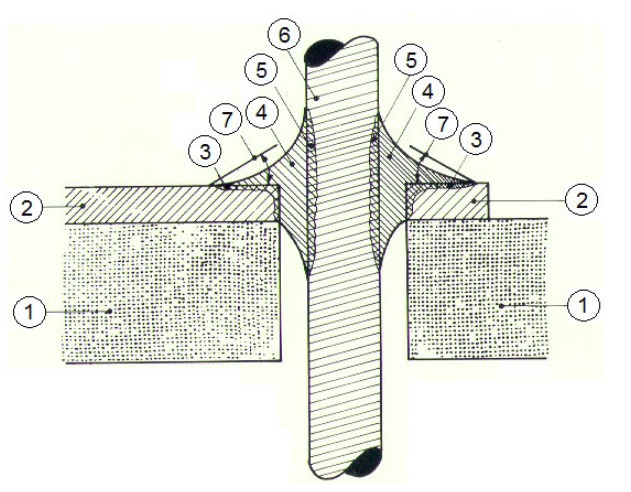
\includegraphics[width=\textwidth]{Figuras/soldagem_ideal.jpeg}
  \caption{Partes de uma PCI e uma soldagem eficiente.} 
 { \footnotesize FONTE (ADAPTADO): "MCE - Montagem de Circuitos Eletrônicos". 
 Wilson Carvalho - ETEC ALBERT EINSTEIN (2014)} 
  \label{fig:Solda Ideal}
\end{figure}

A Figura \ref{fig:Solda Ideal} apresenta os pontos que caracterizam uma solda eficiente. Onde cada ponto é identificado da seguinte forma:

\begin{enumerate}
    \item Substrato da PCI
    \item Camada de cobre
    \item Liga de solda e pista de cobre (somente algumas moléculas de espessura)
    \item Solda
    \item Liga de solda e terminal do componente
    \item Terminal do componente
    \item Ângulo máximo entre a solda e a pista impressa (inferior a 30°)
\end{enumerate}

\newpage

\chapter{Placas de Circuito Impresso}

\section{Confecção das placas de circuito impresso}

\par Para a confecção das placas de circuito impresso foram gerados os arquivos Gerber de cada placa de circuito impresso, sendo gerado um arquivo em formato ZIP disponíveis em Arquivos Gerber sendo fabricadas com 2 Layers com a placa contendo uma espessura de $1.6 mm$ e peso de cobre de $1 oz$. Para a visualização dos arquivos Gerber é necessário a utilização de um programa de prototipagem de placas de circuito impresso ou um visualizador desse tipo de arquivo disponível para download no site do programa utilizado para o projeto EasyEda como pode se observado na figura \ref{fig:Gerber}.
\par Link download arquivos Gerber: \href {https://drive.google.com/drive/folders/1P1pQGE_zuSLOB5qd8zfESWqLDwtyoRKd?usp=sharing}{aqui}
\par Link download do programa vizualizador: \href{https://sourceforge.net/projects/gerbv/files/}{aqui} 

\begin{figure}[H]
  \centering
  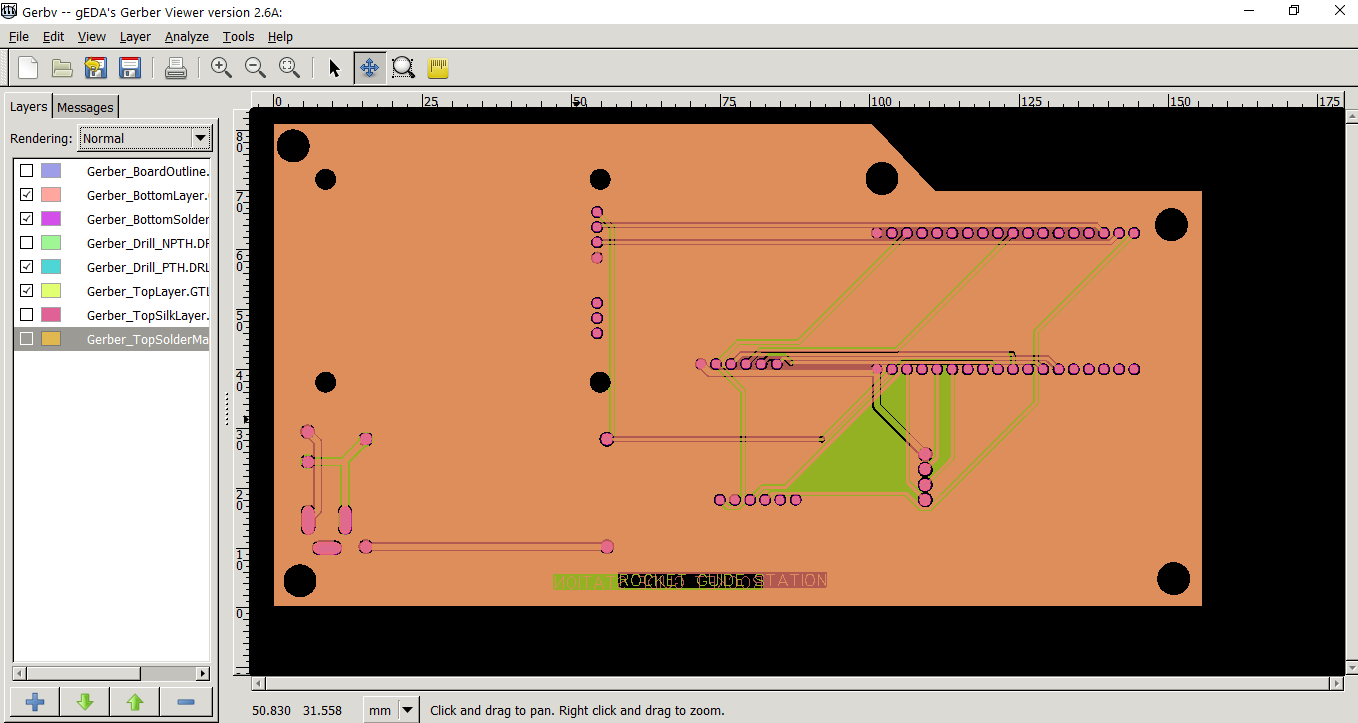
\includegraphics[scale=0.3]{Figuras/pci fabric/imagem de fabicação.png}
  \caption{Programa visualizador do Gerber.}
  \label{fig:Gerber}
\end{figure}

\subsection{Placa de Circuito Impresso-Foguete}
\par Na figura \ref{fig:Gerber da PCI-Foguete} se encontra parte do arquivo Gerber para a fabricação da PCI do foguete e na \ref{fig: PCI-Foguete} se encontra o projeto final de como deve ficar apos a fabricação da mesma.

\begin{figure}[H]
  \centering
  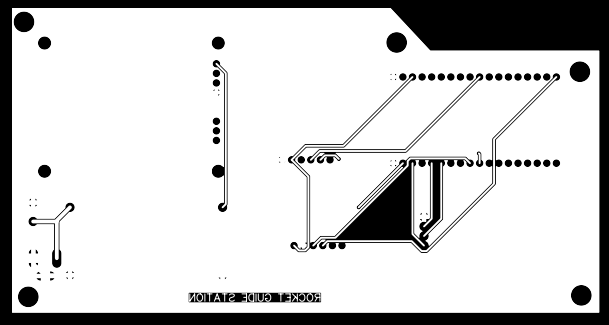
\includegraphics[scale=0.4]{Figuras/pci fabric/gerber foguete bottomlayer.png}
    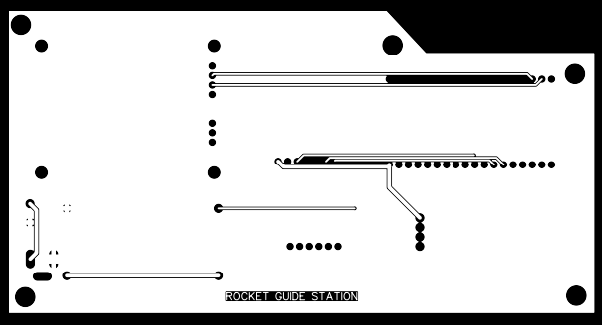
\includegraphics[scale=0.4]{Figuras/pci fabric/gerber foguete toplayer.png}
  \caption{Gerber da PCI-Foguete.}
  \label{fig:Gerber da PCI-Foguete}
\end{figure}

\begin{figure}[H]
  \centering
  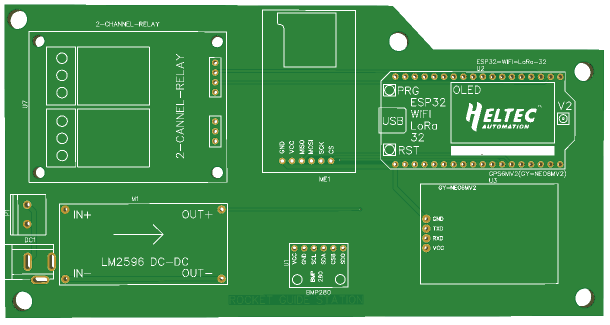
\includegraphics[scale=0.4]{Figuras/pci fabric/foguete_top.png}
    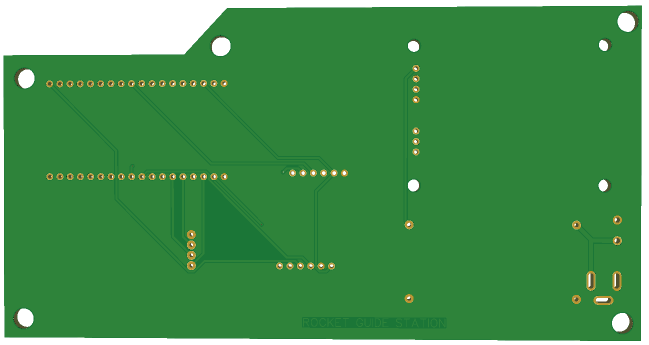
\includegraphics[scale=0.4]{Figuras/pci fabric/foguete_bottom.png}
  \caption{ PCI-Foguete.}
  \label{fig: PCI-Foguete}
\end{figure}

\subsection{Placa de Circuito Impresso-Base de Lançamento}

\par Na figura \ref{fig:Gerber da PCI-Base} se encontra parte do arquivo Gerber para a fabricação da PCI do foguete e na \ref{fig: PCI-Base} se encontra o projeto final de como deve ficar apos a fabricação da mesma.



\begin{figure}[H]
  \centering
  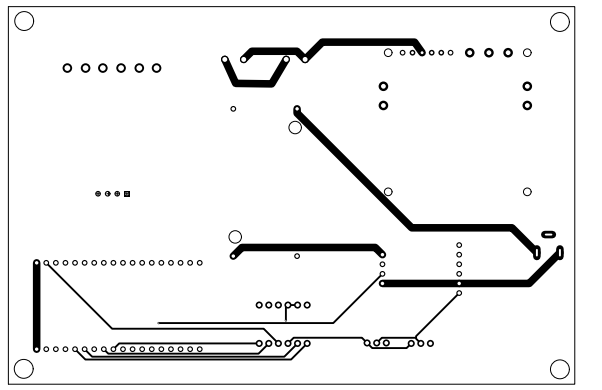
\includegraphics[scale=0.4]{Figuras/pci fabric/gerber base toplayer.png}
    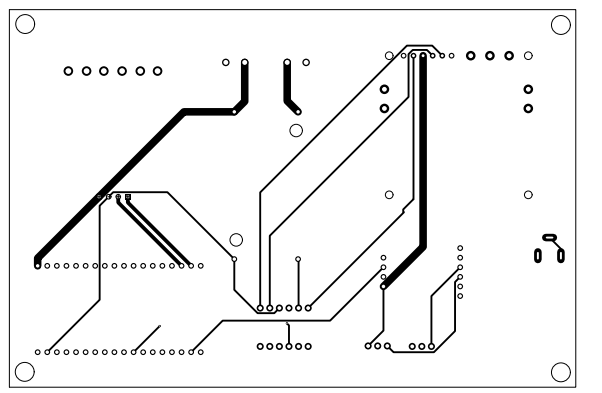
\includegraphics[scale=0.4]{Figuras/pci fabric/gerber base bottom layer.png}
  \caption{Gerber da PCI-Base.}
  \label{fig:Gerber da PCI-Base}
\end{figure}

\begin{figure}[H]
  \centering
  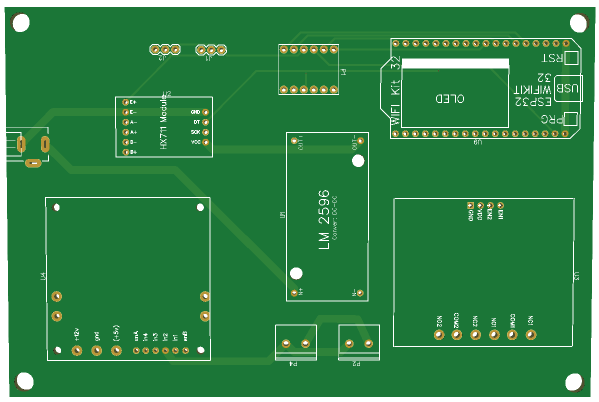
\includegraphics[scale=0.4]{Figuras/pci fabric/BASE_TOP.png}
    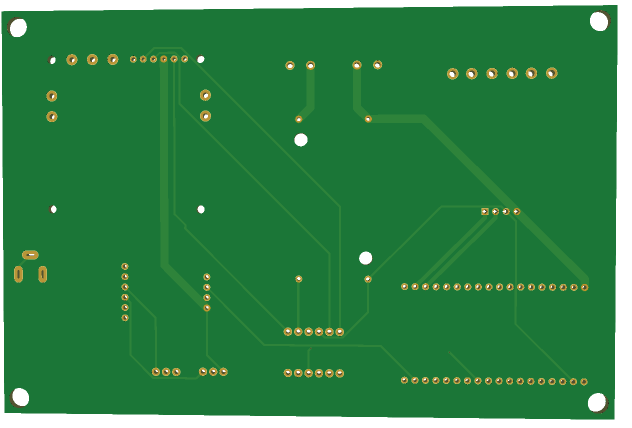
\includegraphics[scale=0.4]{Figuras/pci fabric/BASE_BOTTOM.png}
  \caption{ PCI-Base.}
  \label{fig: PCI-Base}
\end{figure}



\subsection{Placa de Circuito Impresso-Maleta Interface do Usuário}

\par Na figura \ref{fig:Gerber da PCI-Maleta} se encontra parte do arquivo Gerber para a fabricação da PCI do foguete e na \ref{fig: PCI-Maleta} se encontra o projeto final de como deve ficar apos a fabricação da mesma.

\begin{figure}[H]
  \centering
  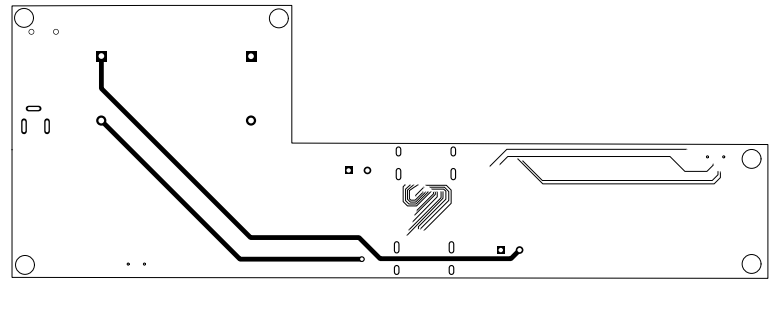
\includegraphics[scale=0.35]{Figuras/pci fabric/gerber maleta bottom layer.png}
    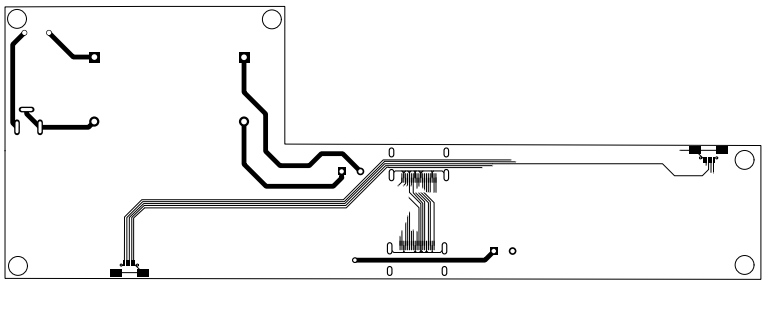
\includegraphics[scale=0.35]{Figuras/pci fabric/gerber maleta toplayer.png}
  \caption{Gerber da PCI-Maleta.}
  \label{fig:Gerber da PCI-Maleta}
\end{figure}


\begin{figure}[H]
  \centering
  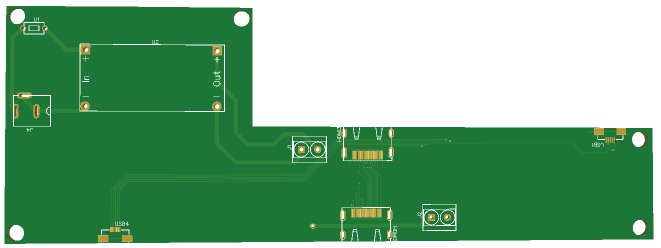
\includegraphics[scale=0.4]{Figuras/pci fabric/maleta_top.png}
    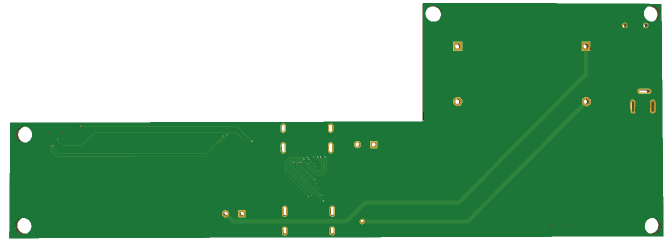
\includegraphics[scale=0.4]{Figuras/pci fabric/maleta_bottom.png}
  \caption{PCI-Maleta.}
  \label{fig: PCI-Maleta}
\end{figure}

\section{Instruções de Montagem das PCI's}
\par A montagem correta das placas é de suma importância para o correto funcionamento do hardware do projeto, siga os passos a seguir para garantir a correta montagem das placas de circuito impresso.
\begin{center}
ATENÇÃO
\begin{figure}[H]
  \centering
  
\includegraphics[scale = 0.1]{Figuras/atenção.png}
\end{figure}
\end{center}



\subsection{Placas de Circuito Impresso-Base de lançamento}
\subsubsection{Lista de Materiais}

\par Primeiramente é necessário ter em mão todos os componentes para sua montagem \ref{fig:Lista de materiasi base}.

\begin{table}[H]
\centering
\begin{tabular}{|m{1.9cm} |m{1.8cm} |m{7.3cm}|m{4cm}|}
\hline
\begin{center}Identificador\end{center} &\begin{center} Quantidade\end{center} & \begin{center}Componente\end{center} &\begin{center} Part Number\end{center} \\\hline
A&01 & PCI- Base & -  \\\hline
B &01&Lora Esp32 Sx1278 Com Display  Oled Wifi bluetooth 915mhz& Sx1278 \\\hline
 
C&01 &  Conversor DC-DC Step Down-LM2596 (12~5V)
& LM2596 \\\hline

D&01&Módulo Conversor Nível Lógico 5V/3.3V -Bidirecional&  MOD-CXI2C \\\hline

E&01&Módulo Hx711 Célula De Carga Balança 24 Bits & HX711 \\\hline

F&01& Driver Motor Ponte H L298n & L298 \\\hline

G&01 &  Módulo Relé 5V 2 Canais &   SRD-05VDC-SL-C \\\hline

H &02& Sensor de Peso 50Kg Célula de Carga & SEN-10245\\\hline

I&01 & Conector Jack J4 DC Fêmea &  Jack Fêmea  \\\hline

J&02&LConector Borne KRE 2 Vias & KRE Kf301 \\\hline

K&04&Parafuso Máquina Cabeça Chata Phillips M5 X 20mm &  Phillips M5 X 20mm \\\hline

L&04& porca de bronze espaçador hexagonal M5 X 12mm & -  \\\hline

\end{tabular}
\caption{Lista de componentes}
\end{table}


\subsubsection{Instruções}

\begin{figure}[H]
  \centering
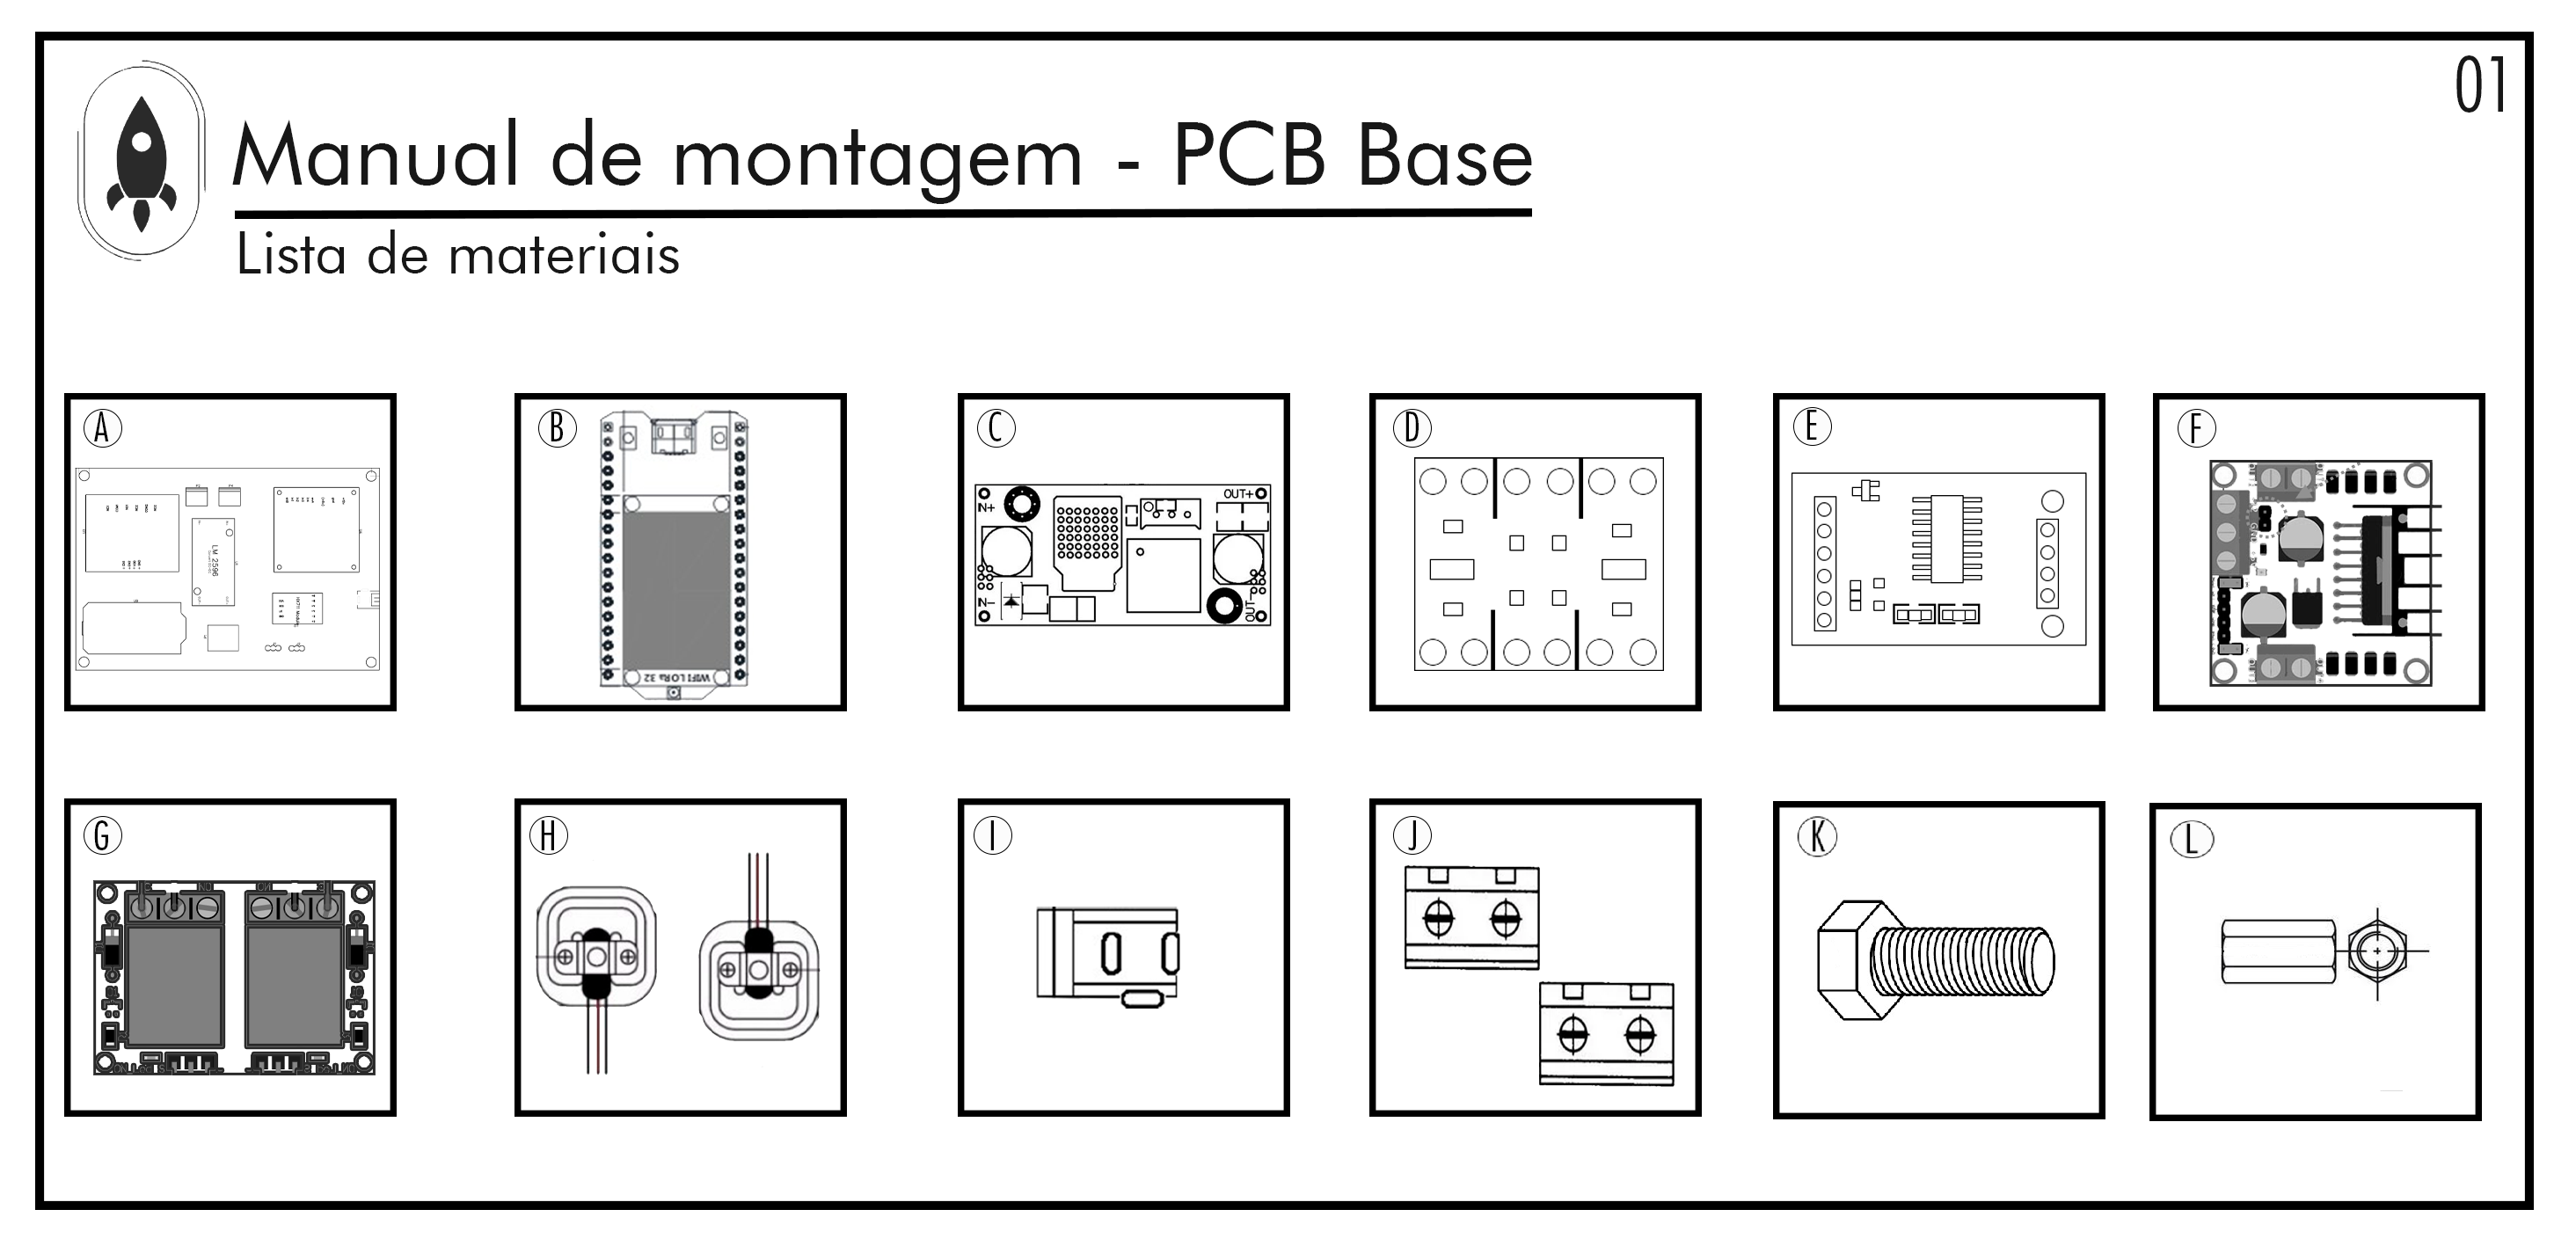
\includegraphics[width=\textwidth]{Figuras/BASE/Pg-01---PL-03.png}
  \caption{Lista de Materiais.} 
 %{ \footnotesize Fonte: Autores} 
 \label{fig:Lista de materiasi base}
 \end{figure}


 \par Com todos os componentes em mãos, pegue componente 'A'(PCI-BASE) prepare-a para soldagem dos componentes passando uma fina camada de solda nos pads da PCI.

\begin{figure}[H]
  \centering
  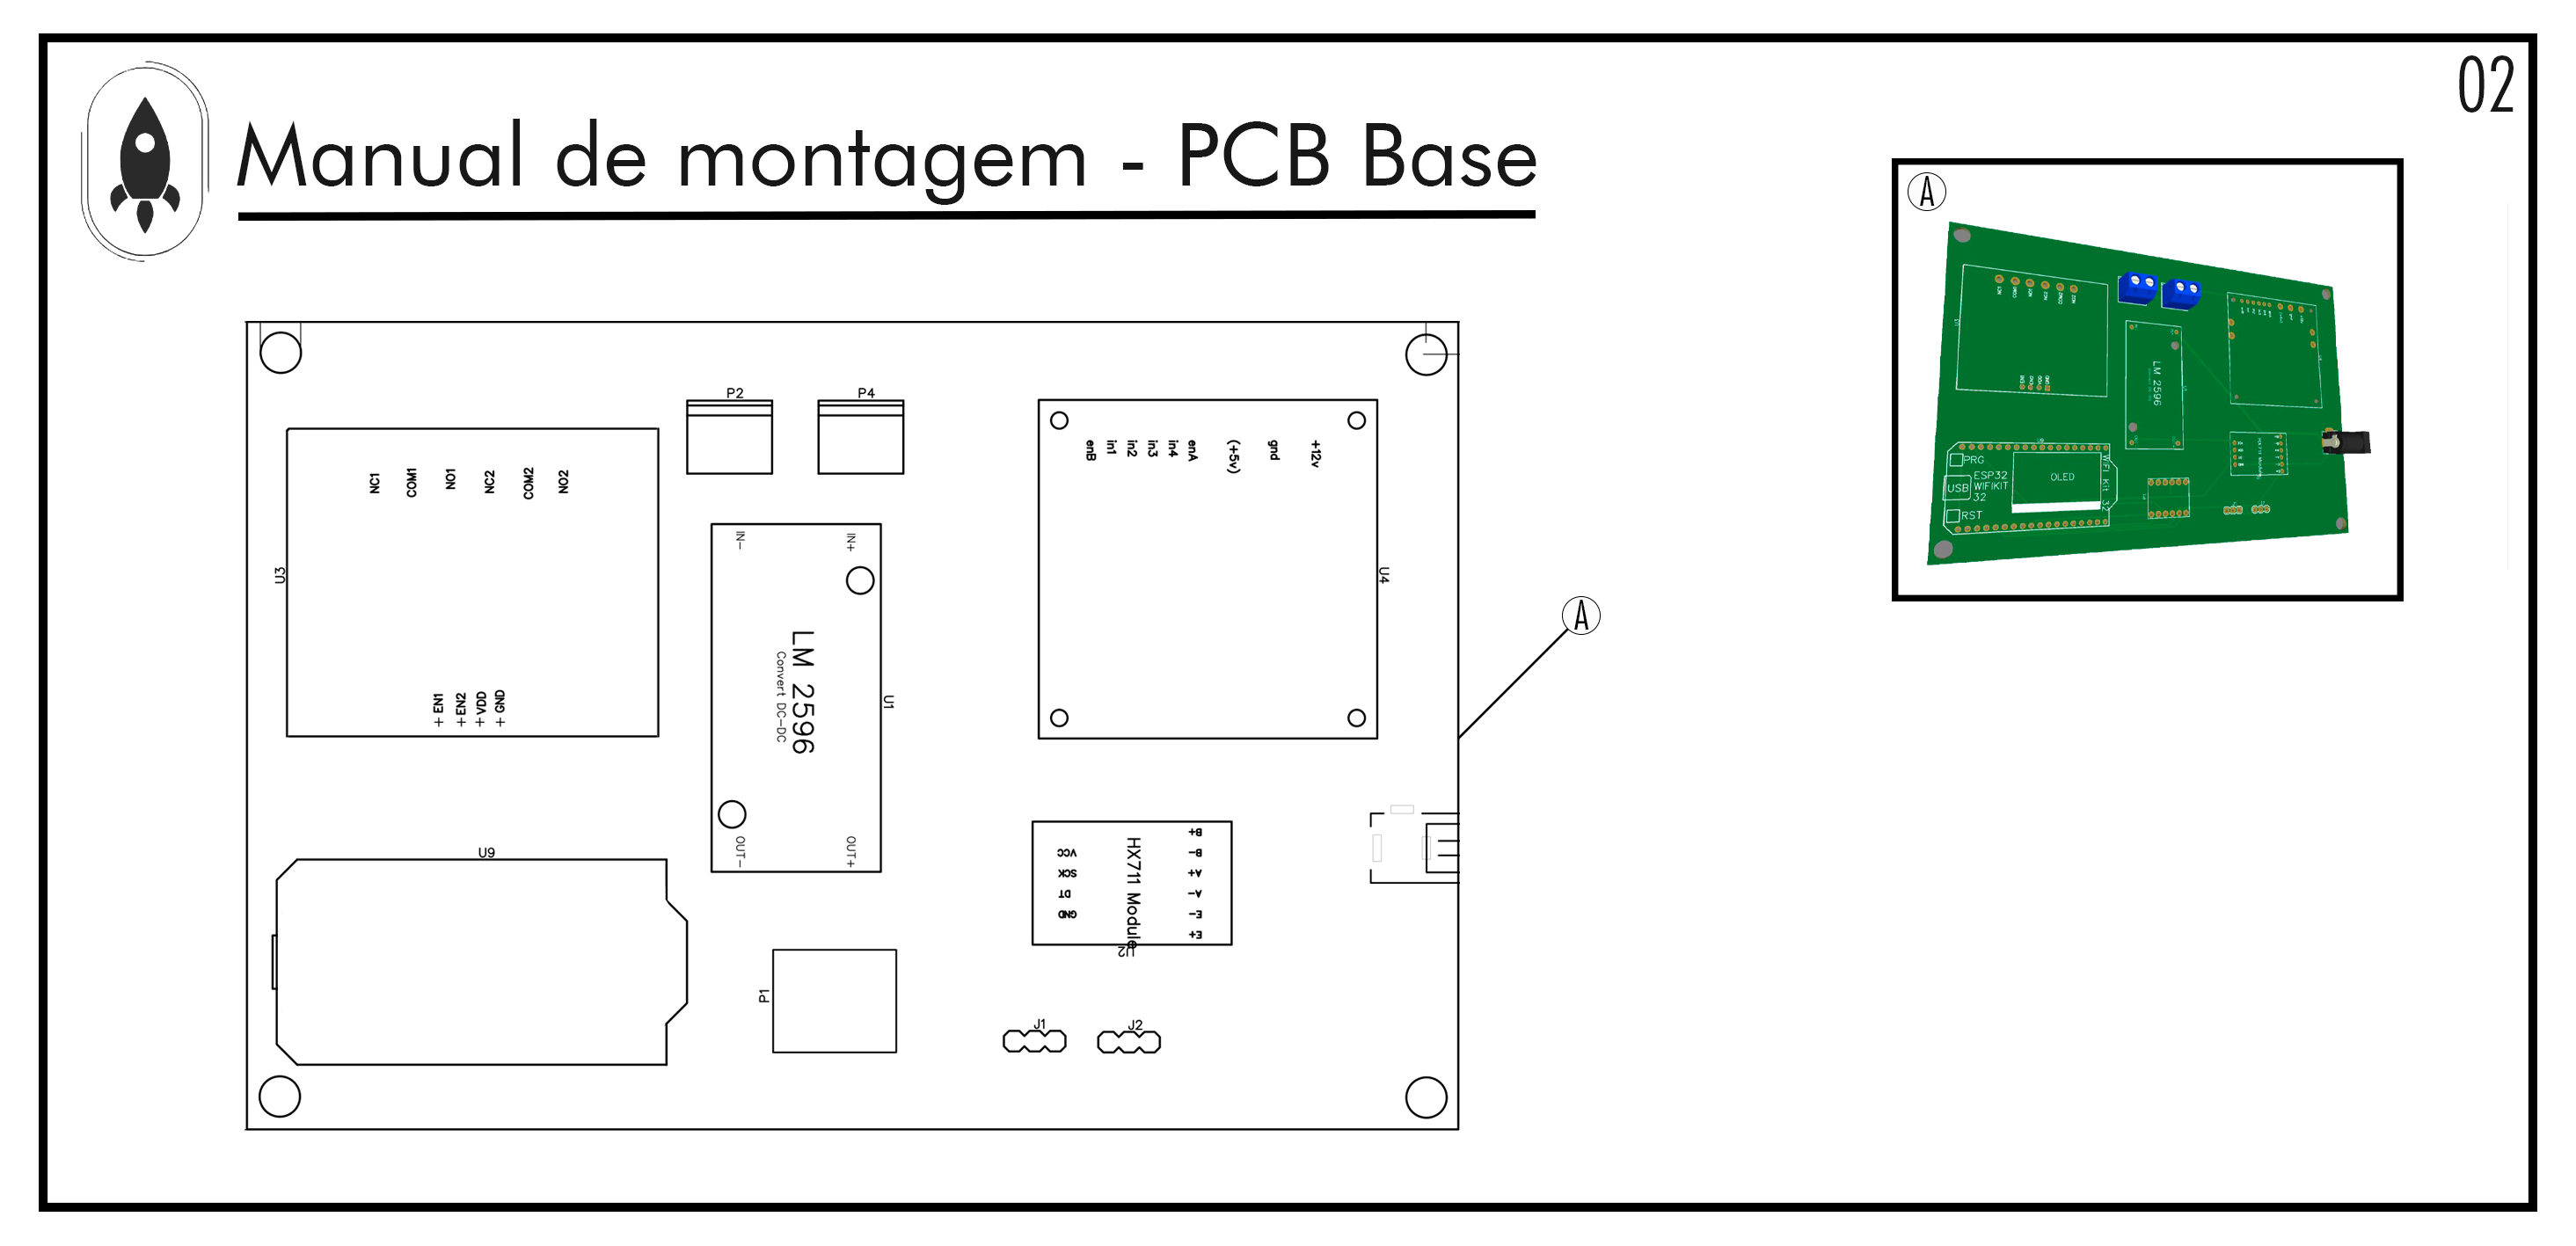
\includegraphics[width=\textwidth]{Figuras/BASE/Pg-02---PL-03.png}
  \caption{PCI da Base.}
 %{ \footnotesize Fonte: Autores} 
  \label{fig:PCIBASE}
\end{figure}

\newpage
\par Pegue o componente 'B'(ESP32 LoRa WiFi), encaixe-a na posição mostrada \ref{fig:PCIBASE LORA} e solde junto a placa.
\begin{figure}[H]
  \centering
  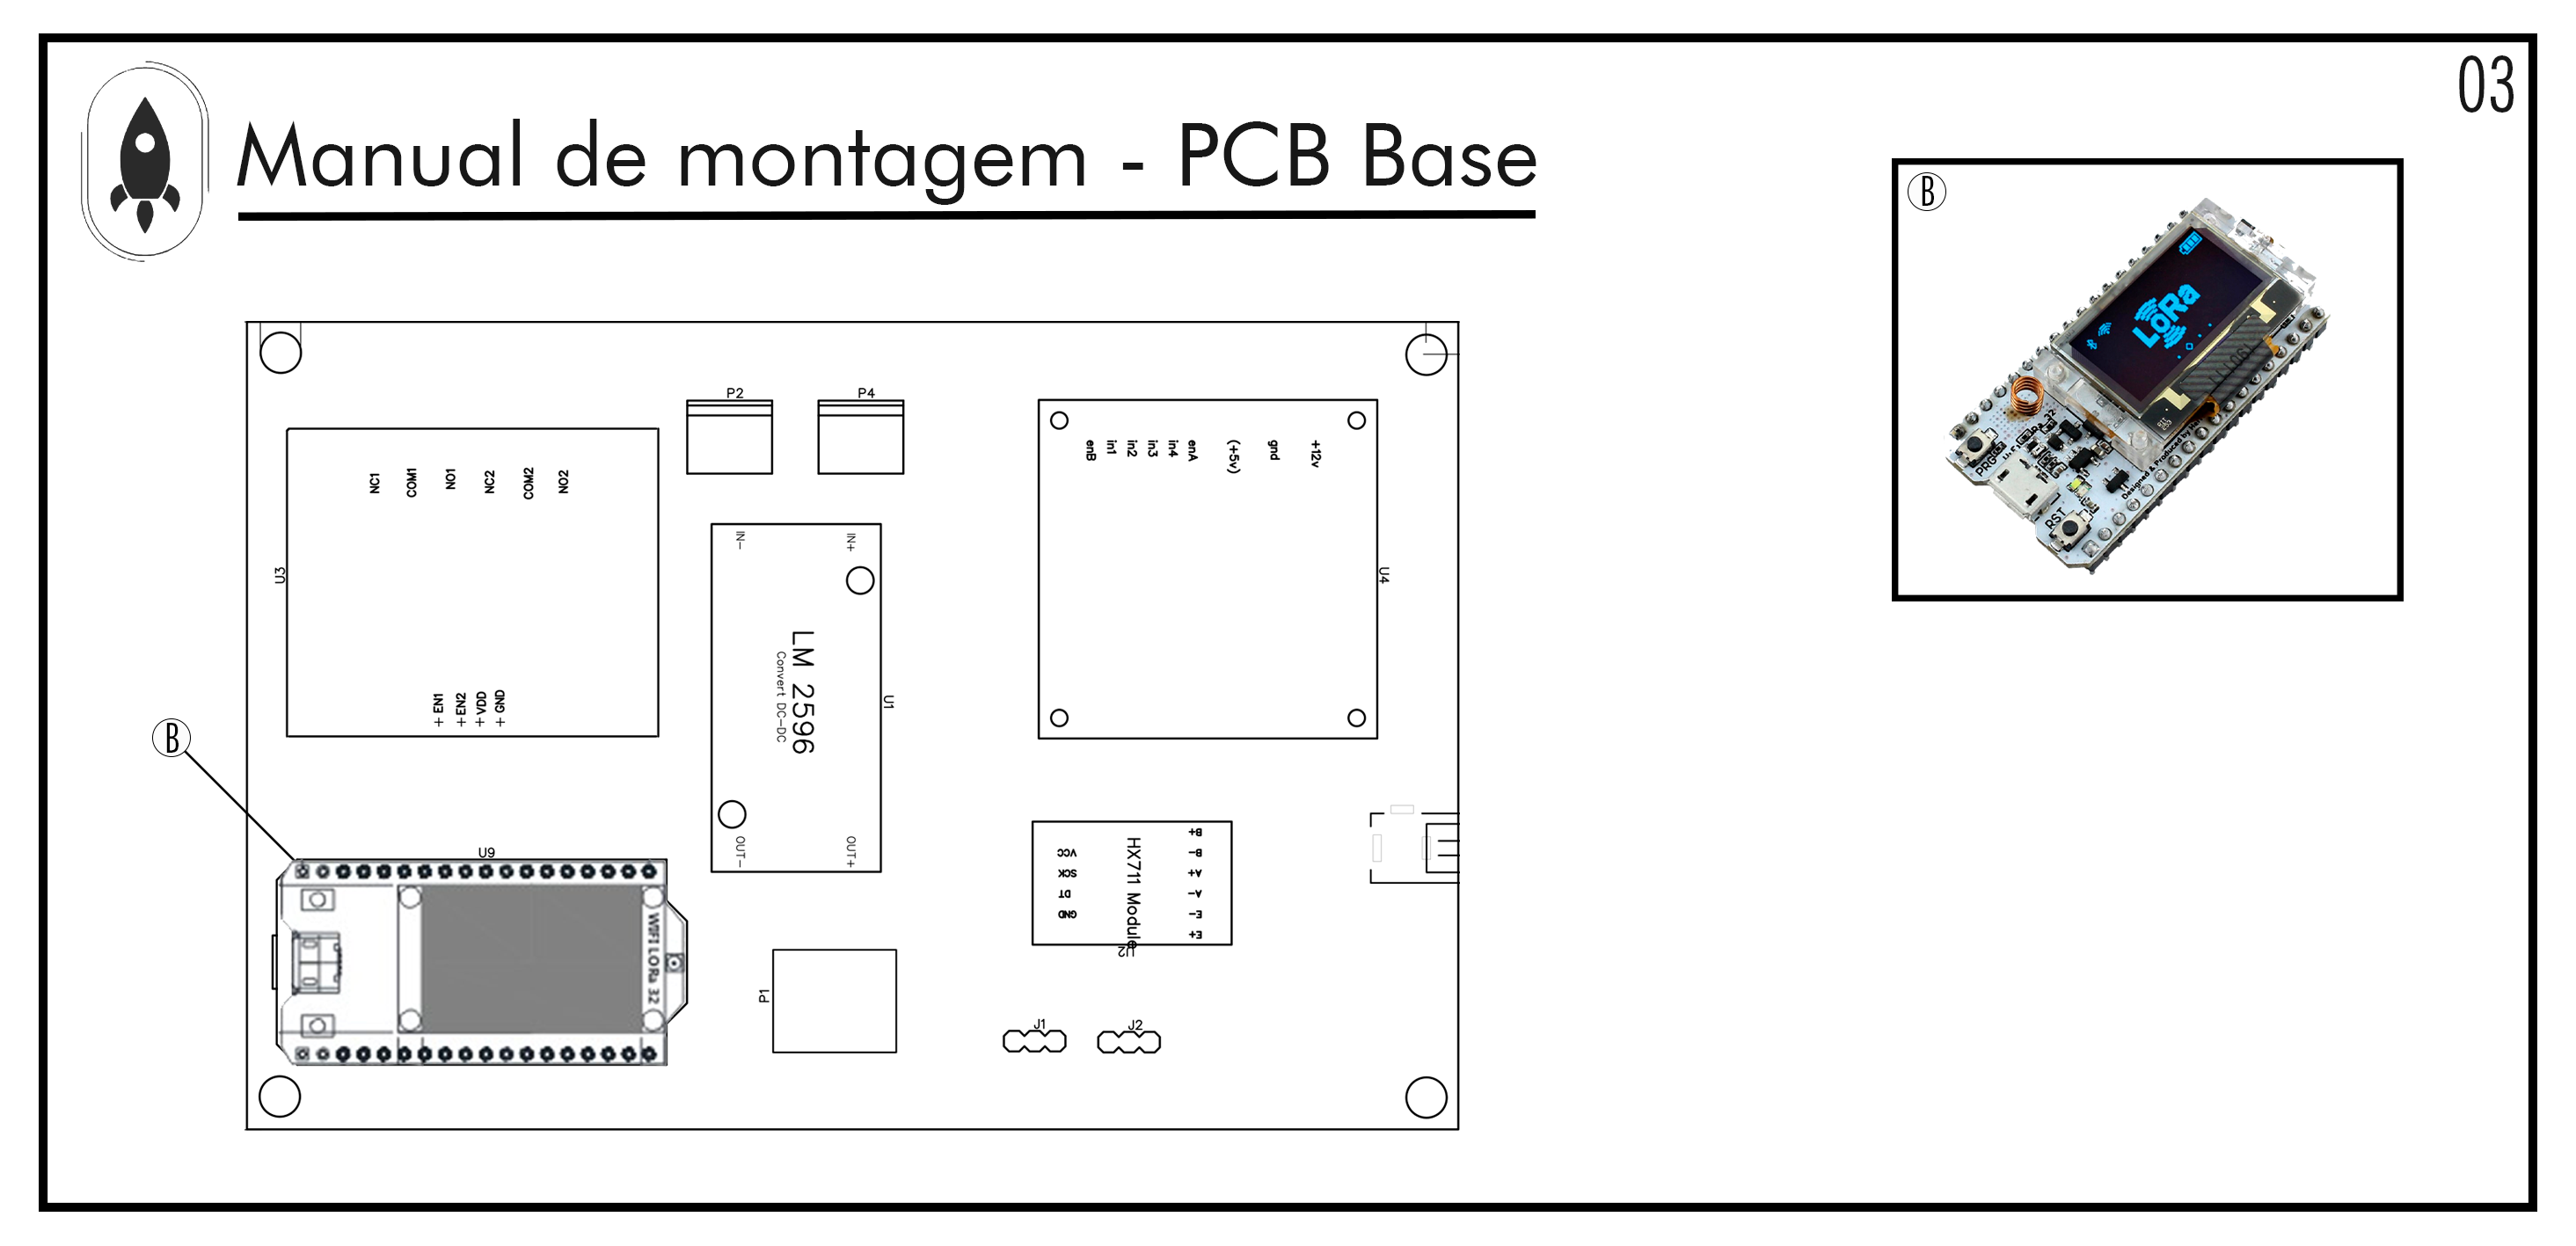
\includegraphics[width=\textwidth]{Figuras/BASE/Pg-03---PL-03.png}
  \caption{ESP32 WiFi Lora.}
 %{ \footnotesize Fonte: Autores} 
  \label{fig:PCIBASE LORA}
\end{figure}


\par Pegue o componente 'C'(LM2596), encaixe-a na posição mostrada \ref{fig:PCIBASE LM2596} e solde junto a placa.
\begin{figure}[H]
  \centering
  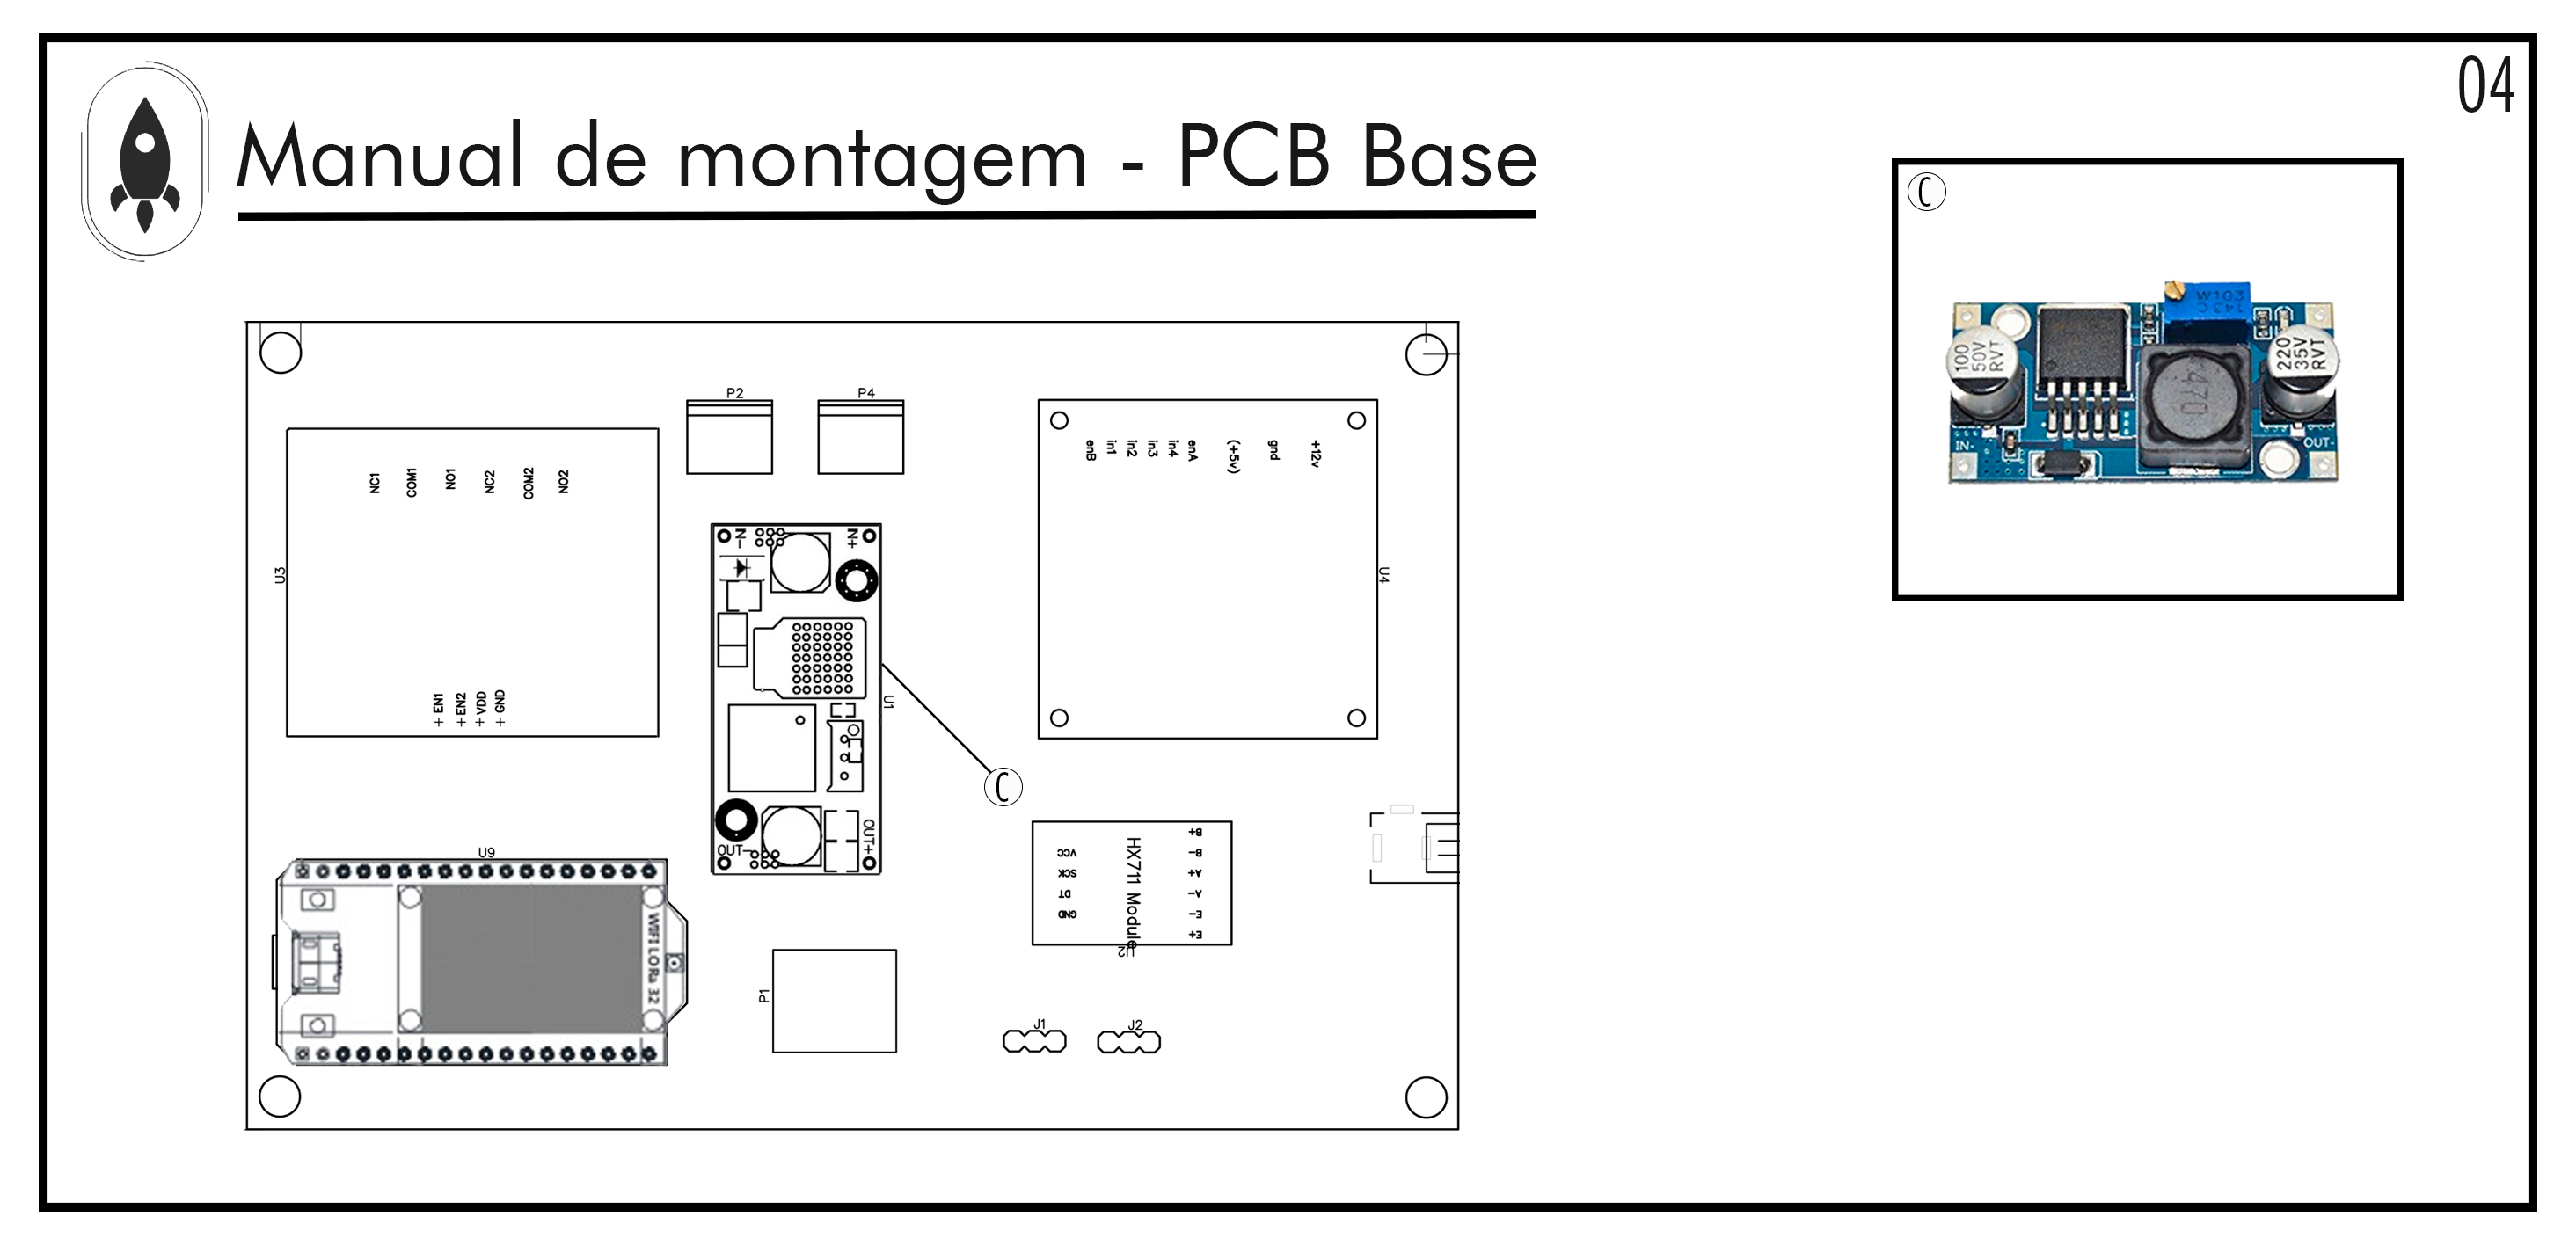
\includegraphics[width=\textwidth]{Figuras/BASE/Pg-04---PL-03.png}
  \caption{LM2596.}
 %{ \footnotesize Fonte: Autores} 
  \label{fig:PCIBASE LM2596}
\end{figure}
\newpage

\par Pegue o componente 'D'(Módulo Conversor Nível Lógico 5V/3.3V -Bidirecional), encaixe-a na posição mostrada \ref{fig:PCIBASE Módulo CONVERSOR LOG  } e solde junto a placa.
\begin{figure}[H]
  \centering
  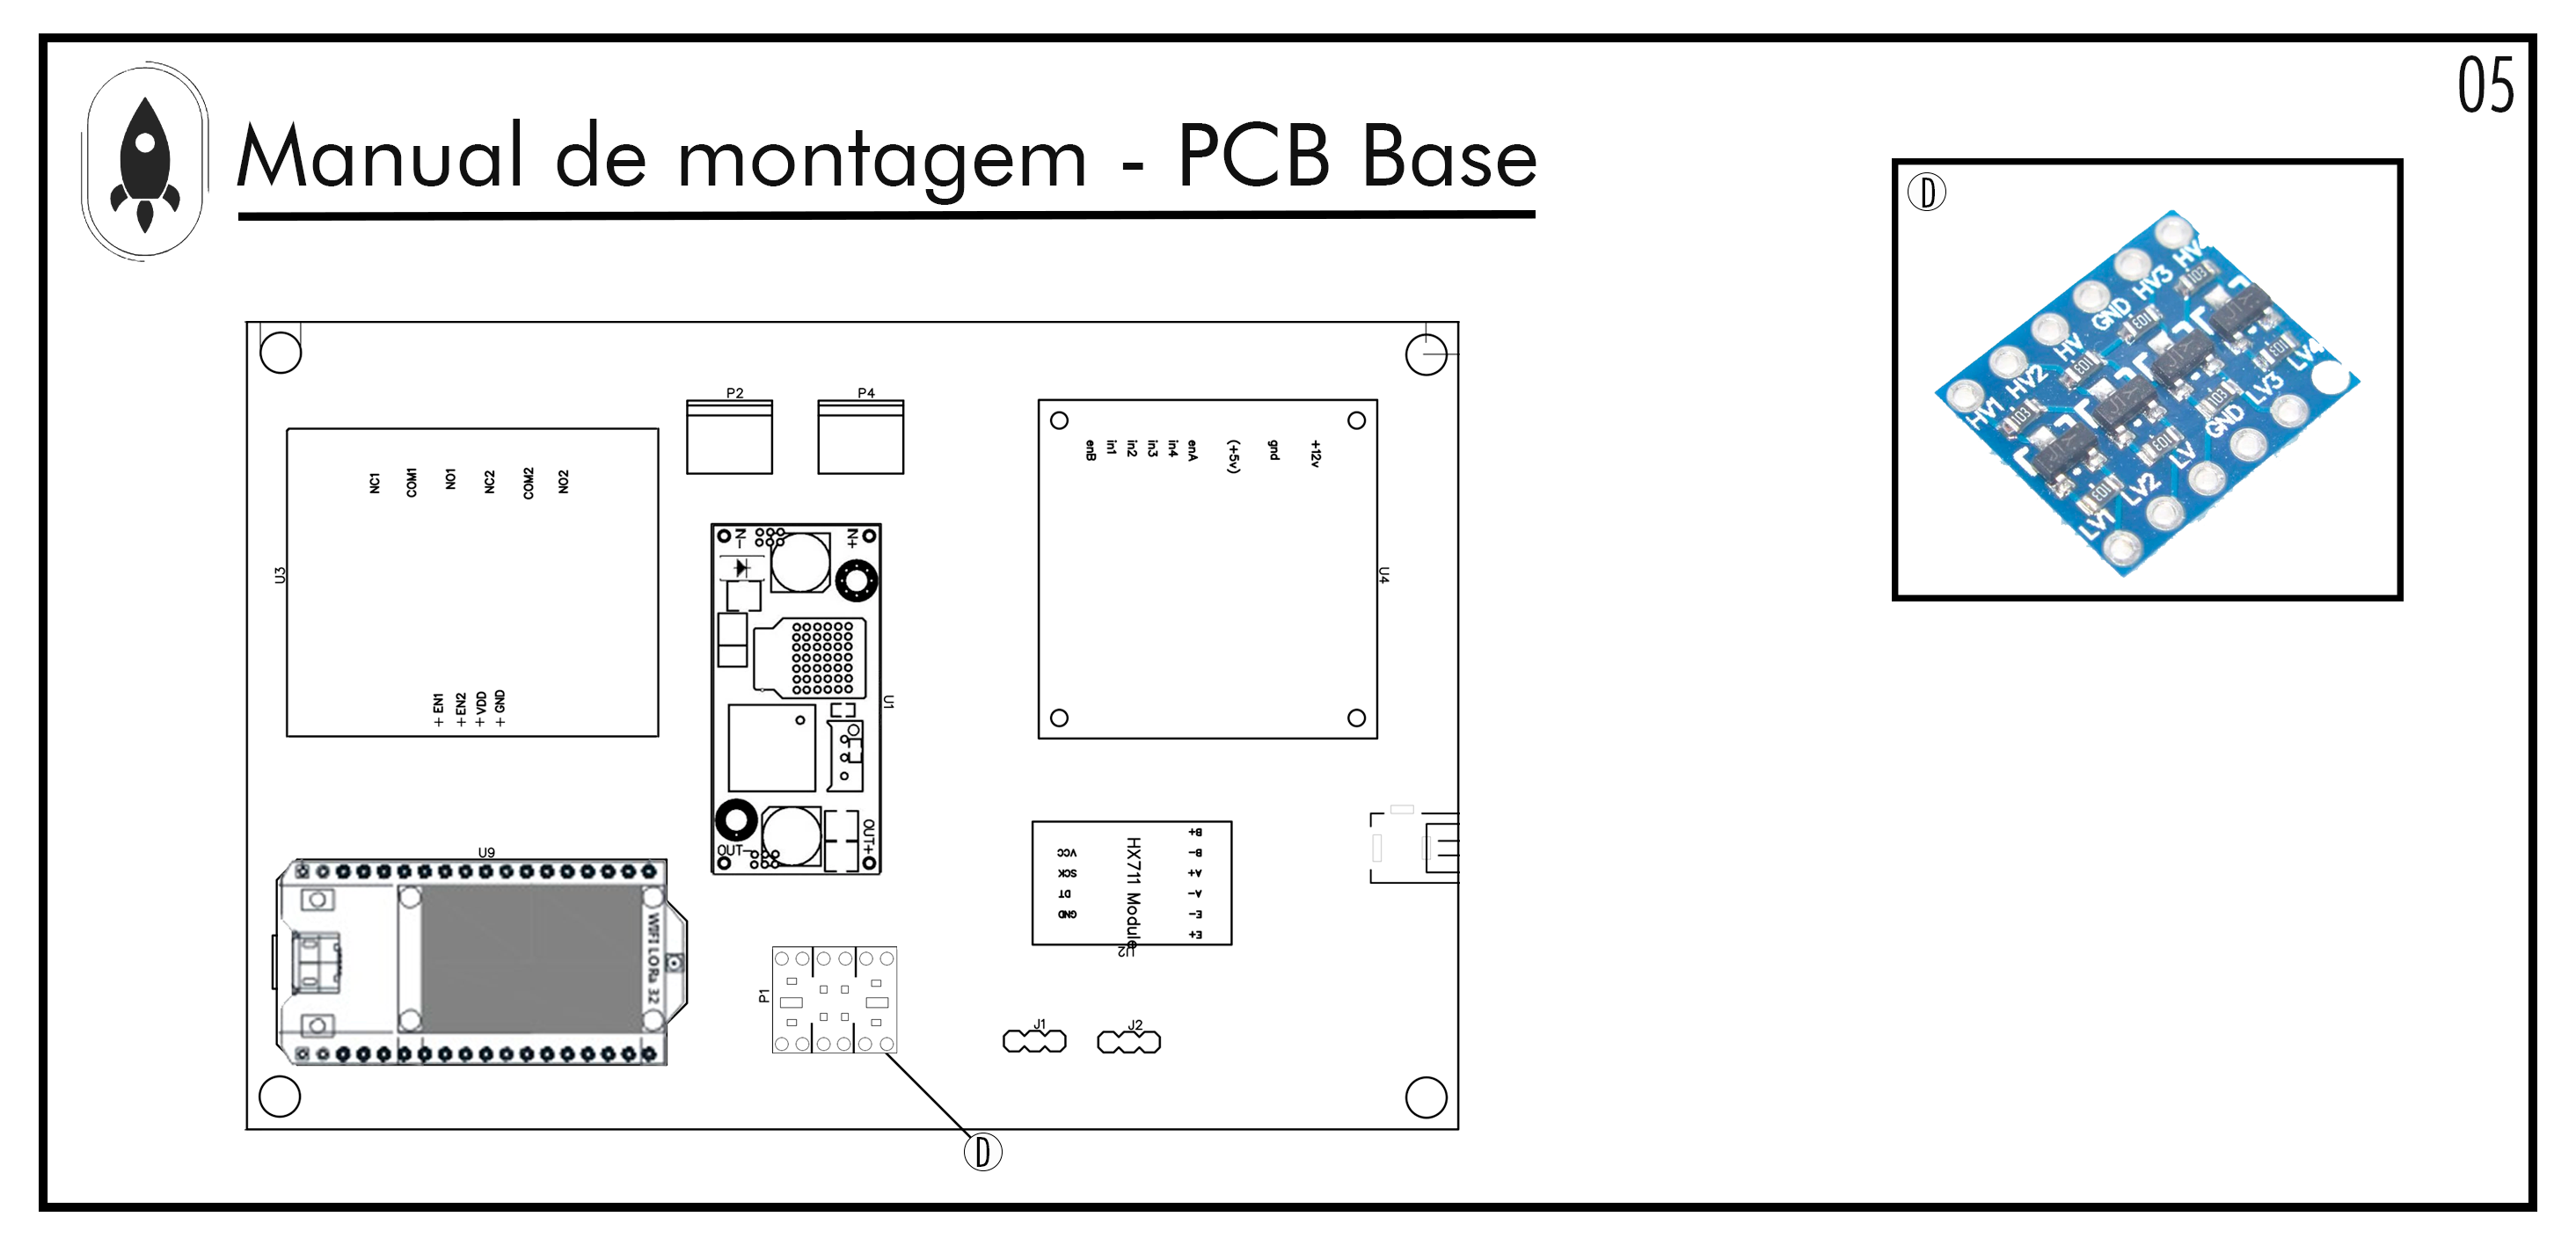
\includegraphics[width=\textwidth]{Figuras/BASE/Pg-05---PL-03.png}
  \caption{Módulo Hx711.}
 %{ \footnotesize Fonte: Autores} 
  \label{fig:PCIBASE Módulo CONVERSOR LOG  }
\end{figure}

\par Pegue o componente 'E'(Módulo Hx711 Célula De Carga Balança 24Bit), encaixe-a na posição mostrada \ref{fig:PCIBASE Módulo Hx711  } e solde junto a placa.
\begin{figure}[H]
  \centering
  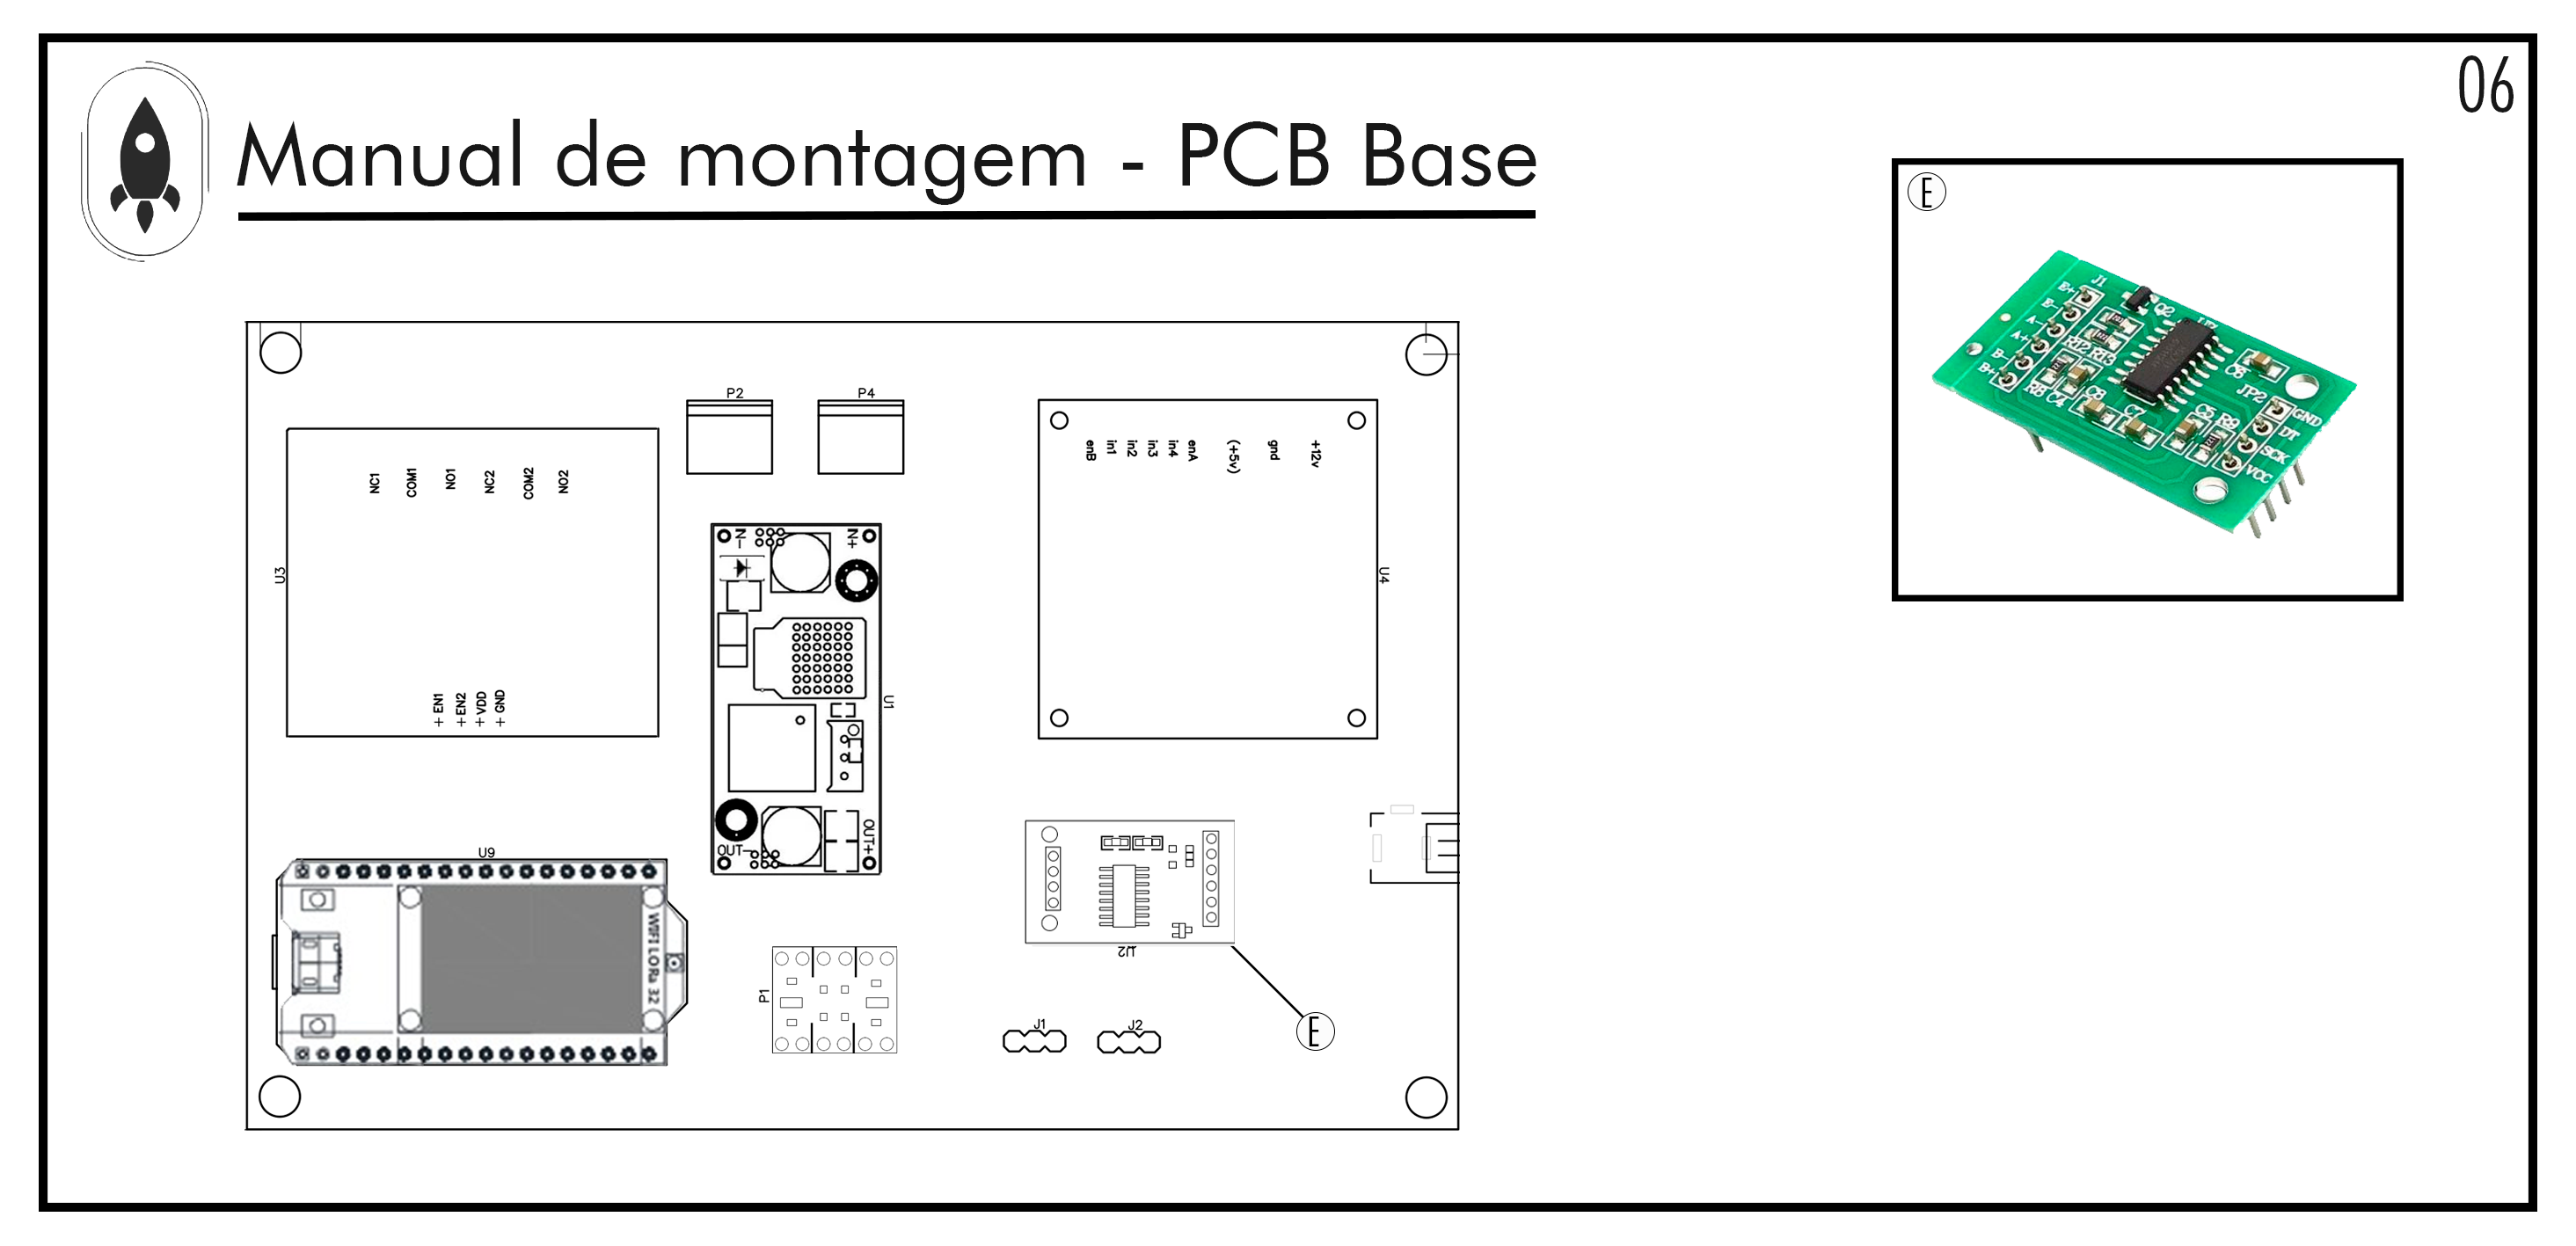
\includegraphics[width=\textwidth]{Figuras/BASE/Pg-06---PL-03.png}
  \caption{Módulo Hx711.}
 %{ \footnotesize Fonte: Autores} 
  \label{fig:PCIBASE Módulo Hx711  }
\end{figure}



\newpage

\par Pegue o componente 'F'(Driver Motor Ponte H L298N), encaixe-a na posição mostrada \ref{fig:PCIBASE ponte H   } e solde junto a placa.
\begin{figure}[H]
  \centering
  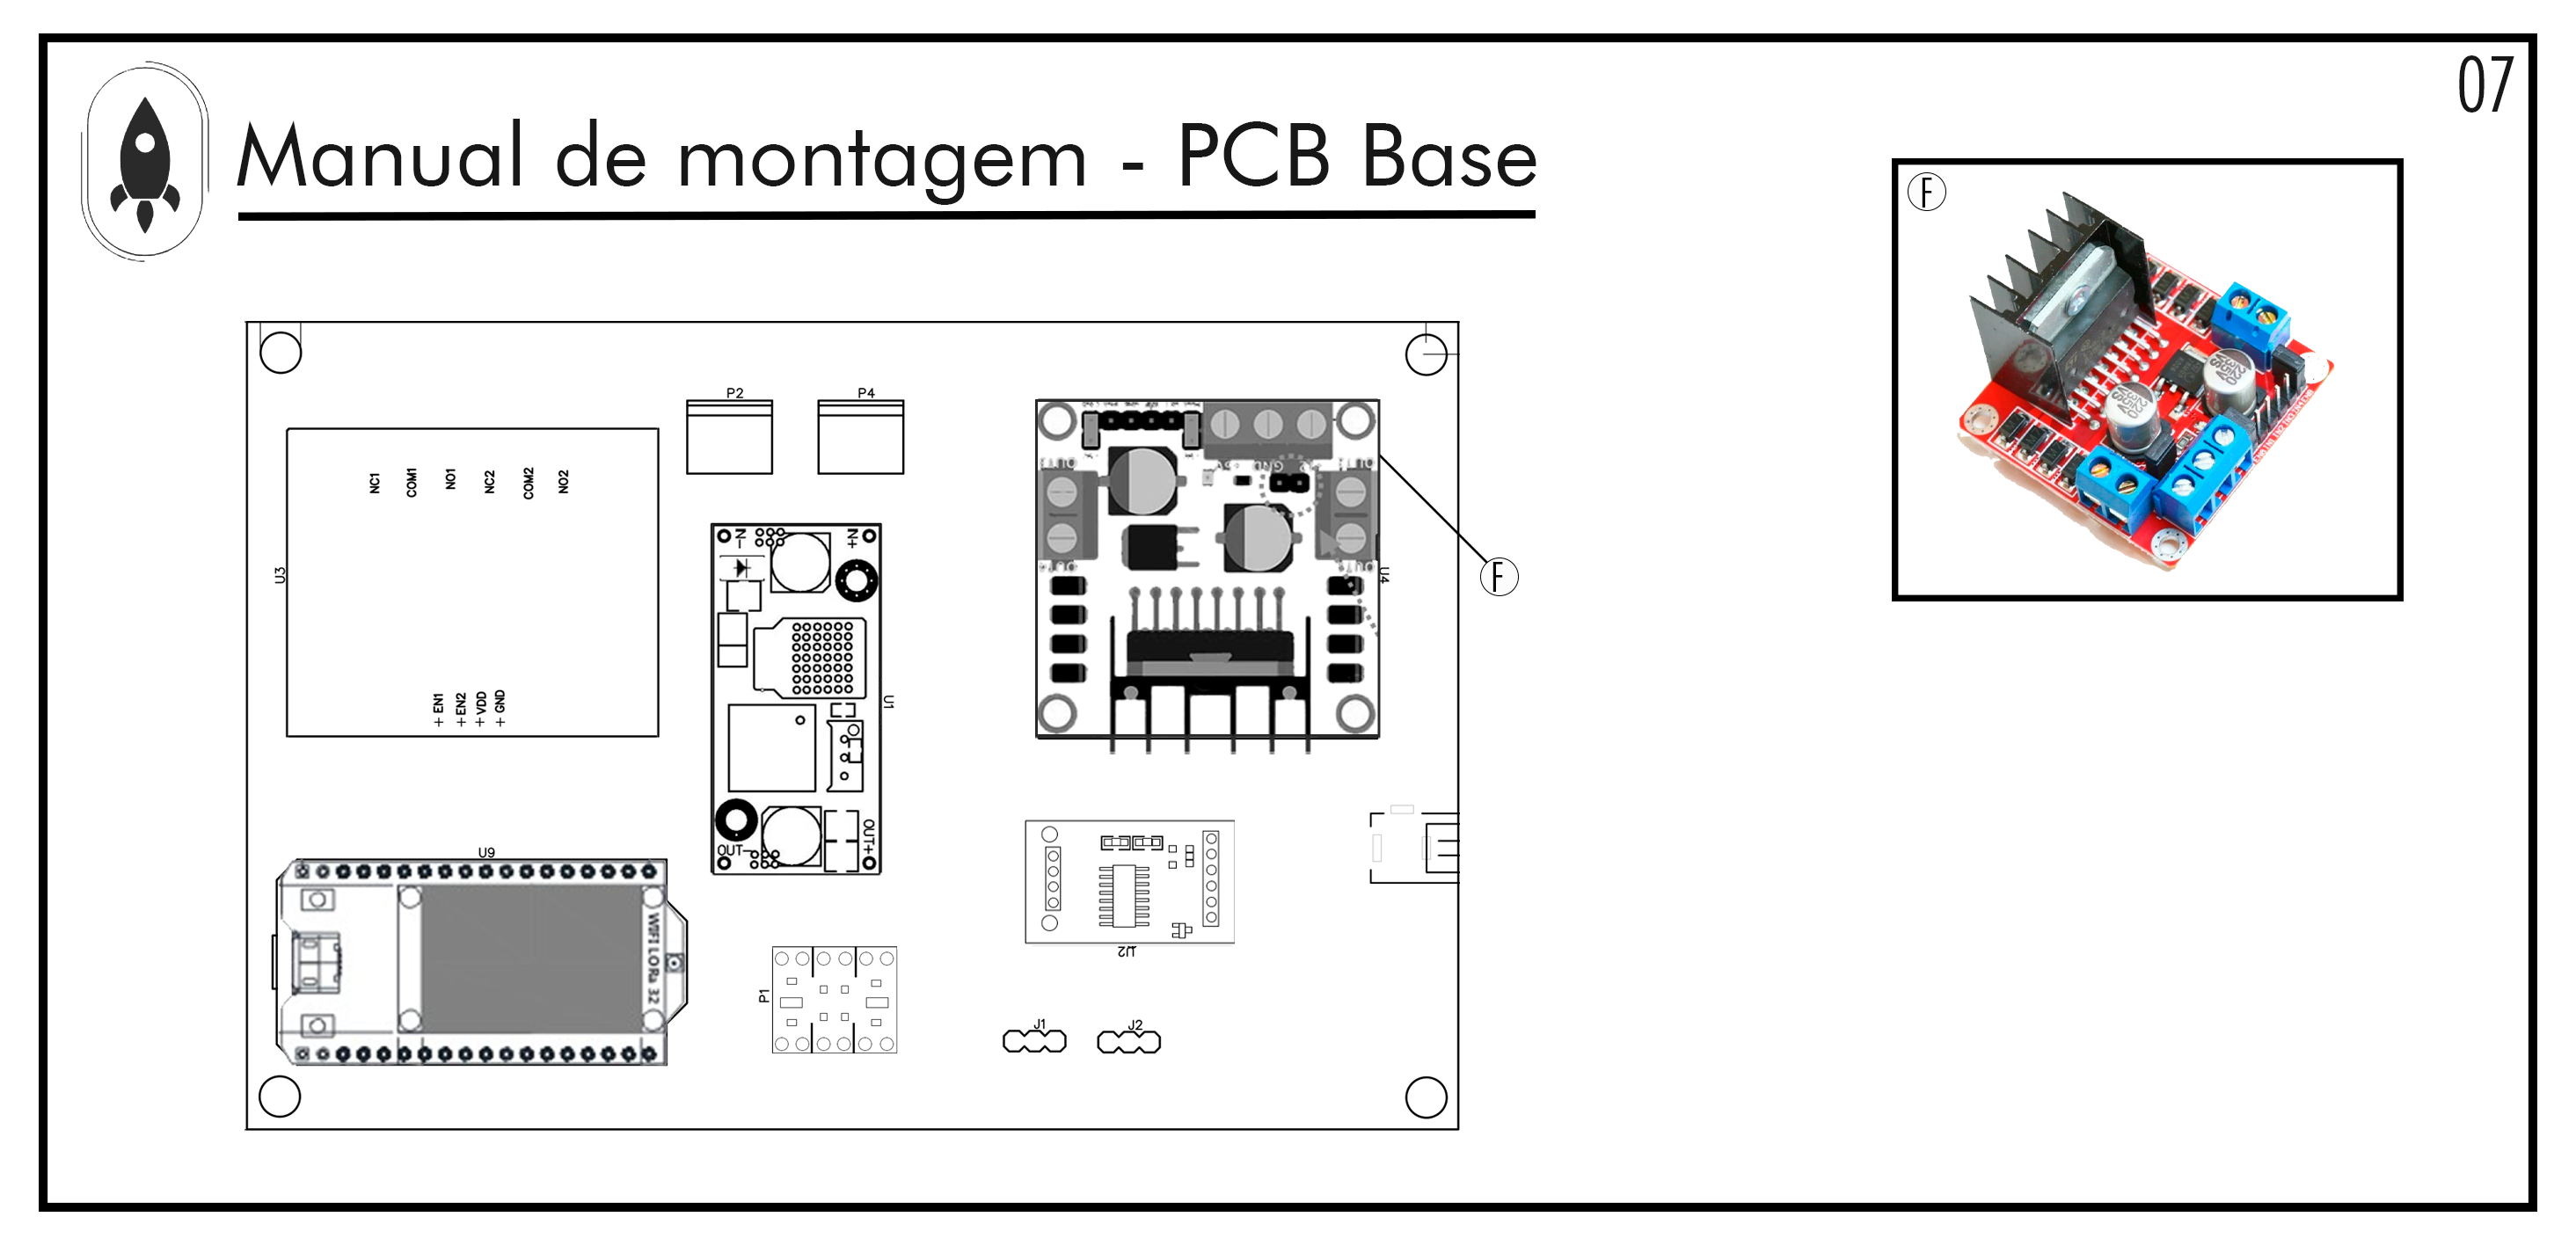
\includegraphics[width=\textwidth]{Figuras/BASE/Pg-07---PL-03.png}
  \caption{Driver Motor Ponte H L298N.}
 %{ \footnotesize Fonte: Autores} 
  \label{fig:PCIBASE ponte H  }
\end{figure}

\par Pegue o componente 'G'( Módulo Relé 5V 2 Canais modelo SRD-05VDC-SL-C), encaixe-a na posição mostrada \ref{fig:PCIBASE Módulo Relé 5V 2 Canais modelo SRD-05VDC-SL-C } e solde junto a placa.
\begin{figure}[H]
  \centering
  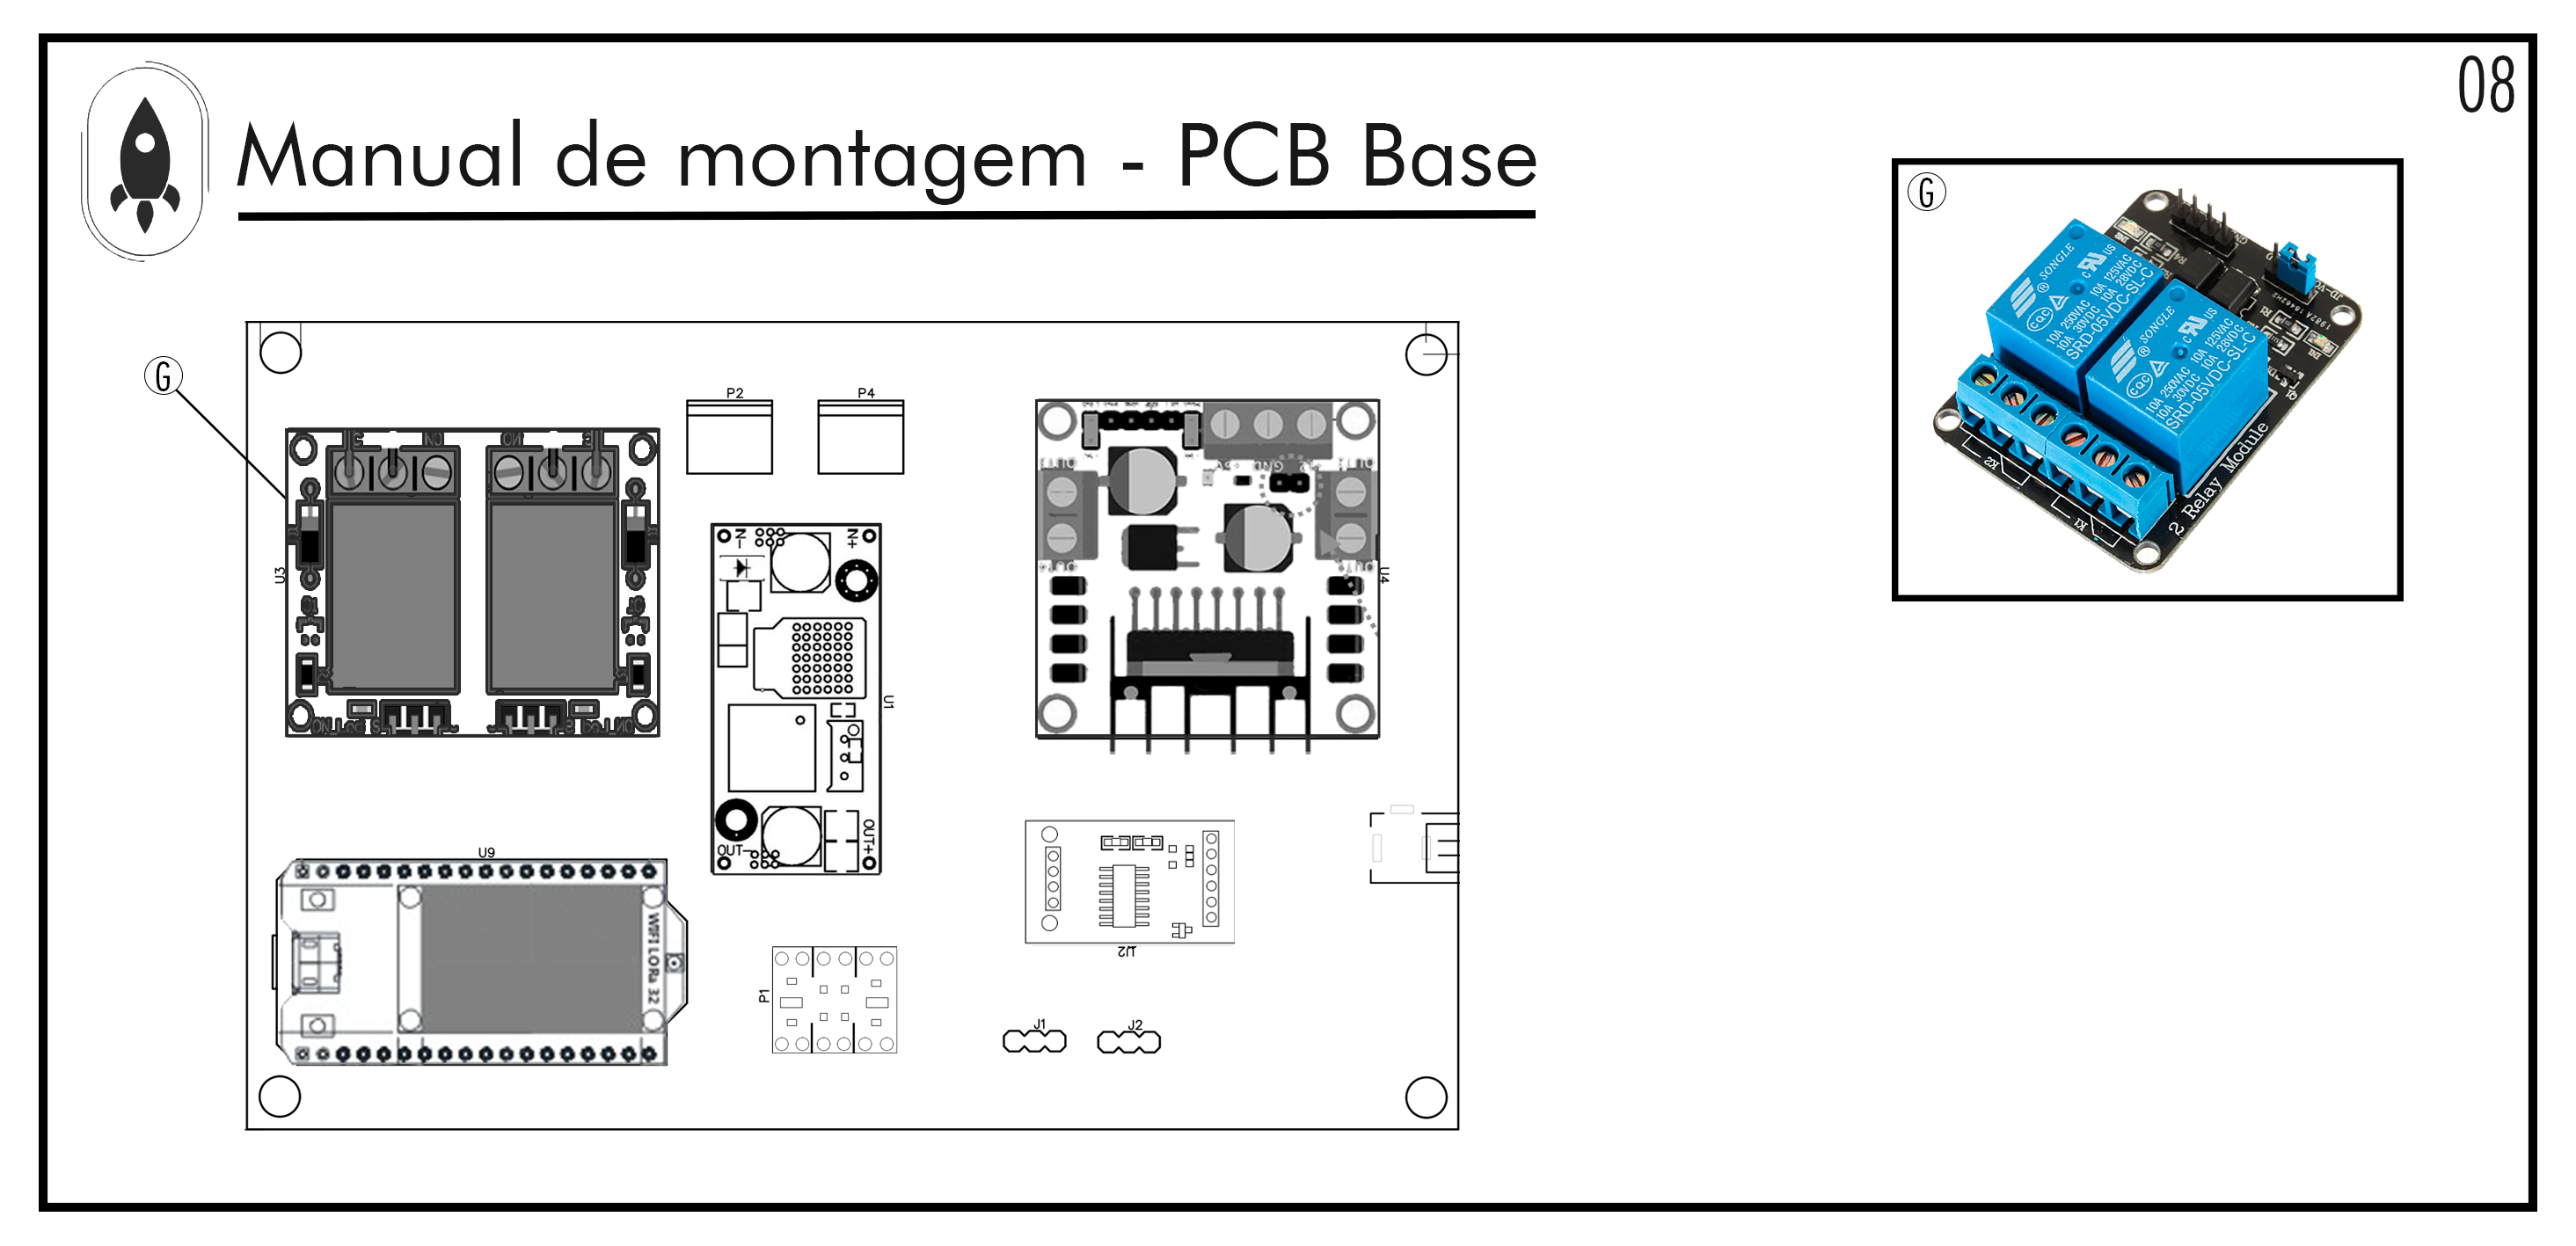
\includegraphics[width=\textwidth]{Figuras/BASE/Pg-08---PL-03.png}
  \caption{ Módulo Relé 5V 2 Canais modelo SRD-05VDC-SL-C.}
 %{ \footnotesize Fonte: Autores} 
  \label{fig:PCIBASE Módulo Relé 5V 2 Canais modelo SRD-05VDC-SL-C }
\end{figure}
\newpage

\par Pegue o componente 'H'(Sensor de Peso 50Kg Célula de Carga ), encaixe-a na posição mostrada \ref{fig:PCIBASE Sensor de Peso 50Kg Célula de Carga  }   e solde junto a placa.
\begin{figure}[H]
  \centering
  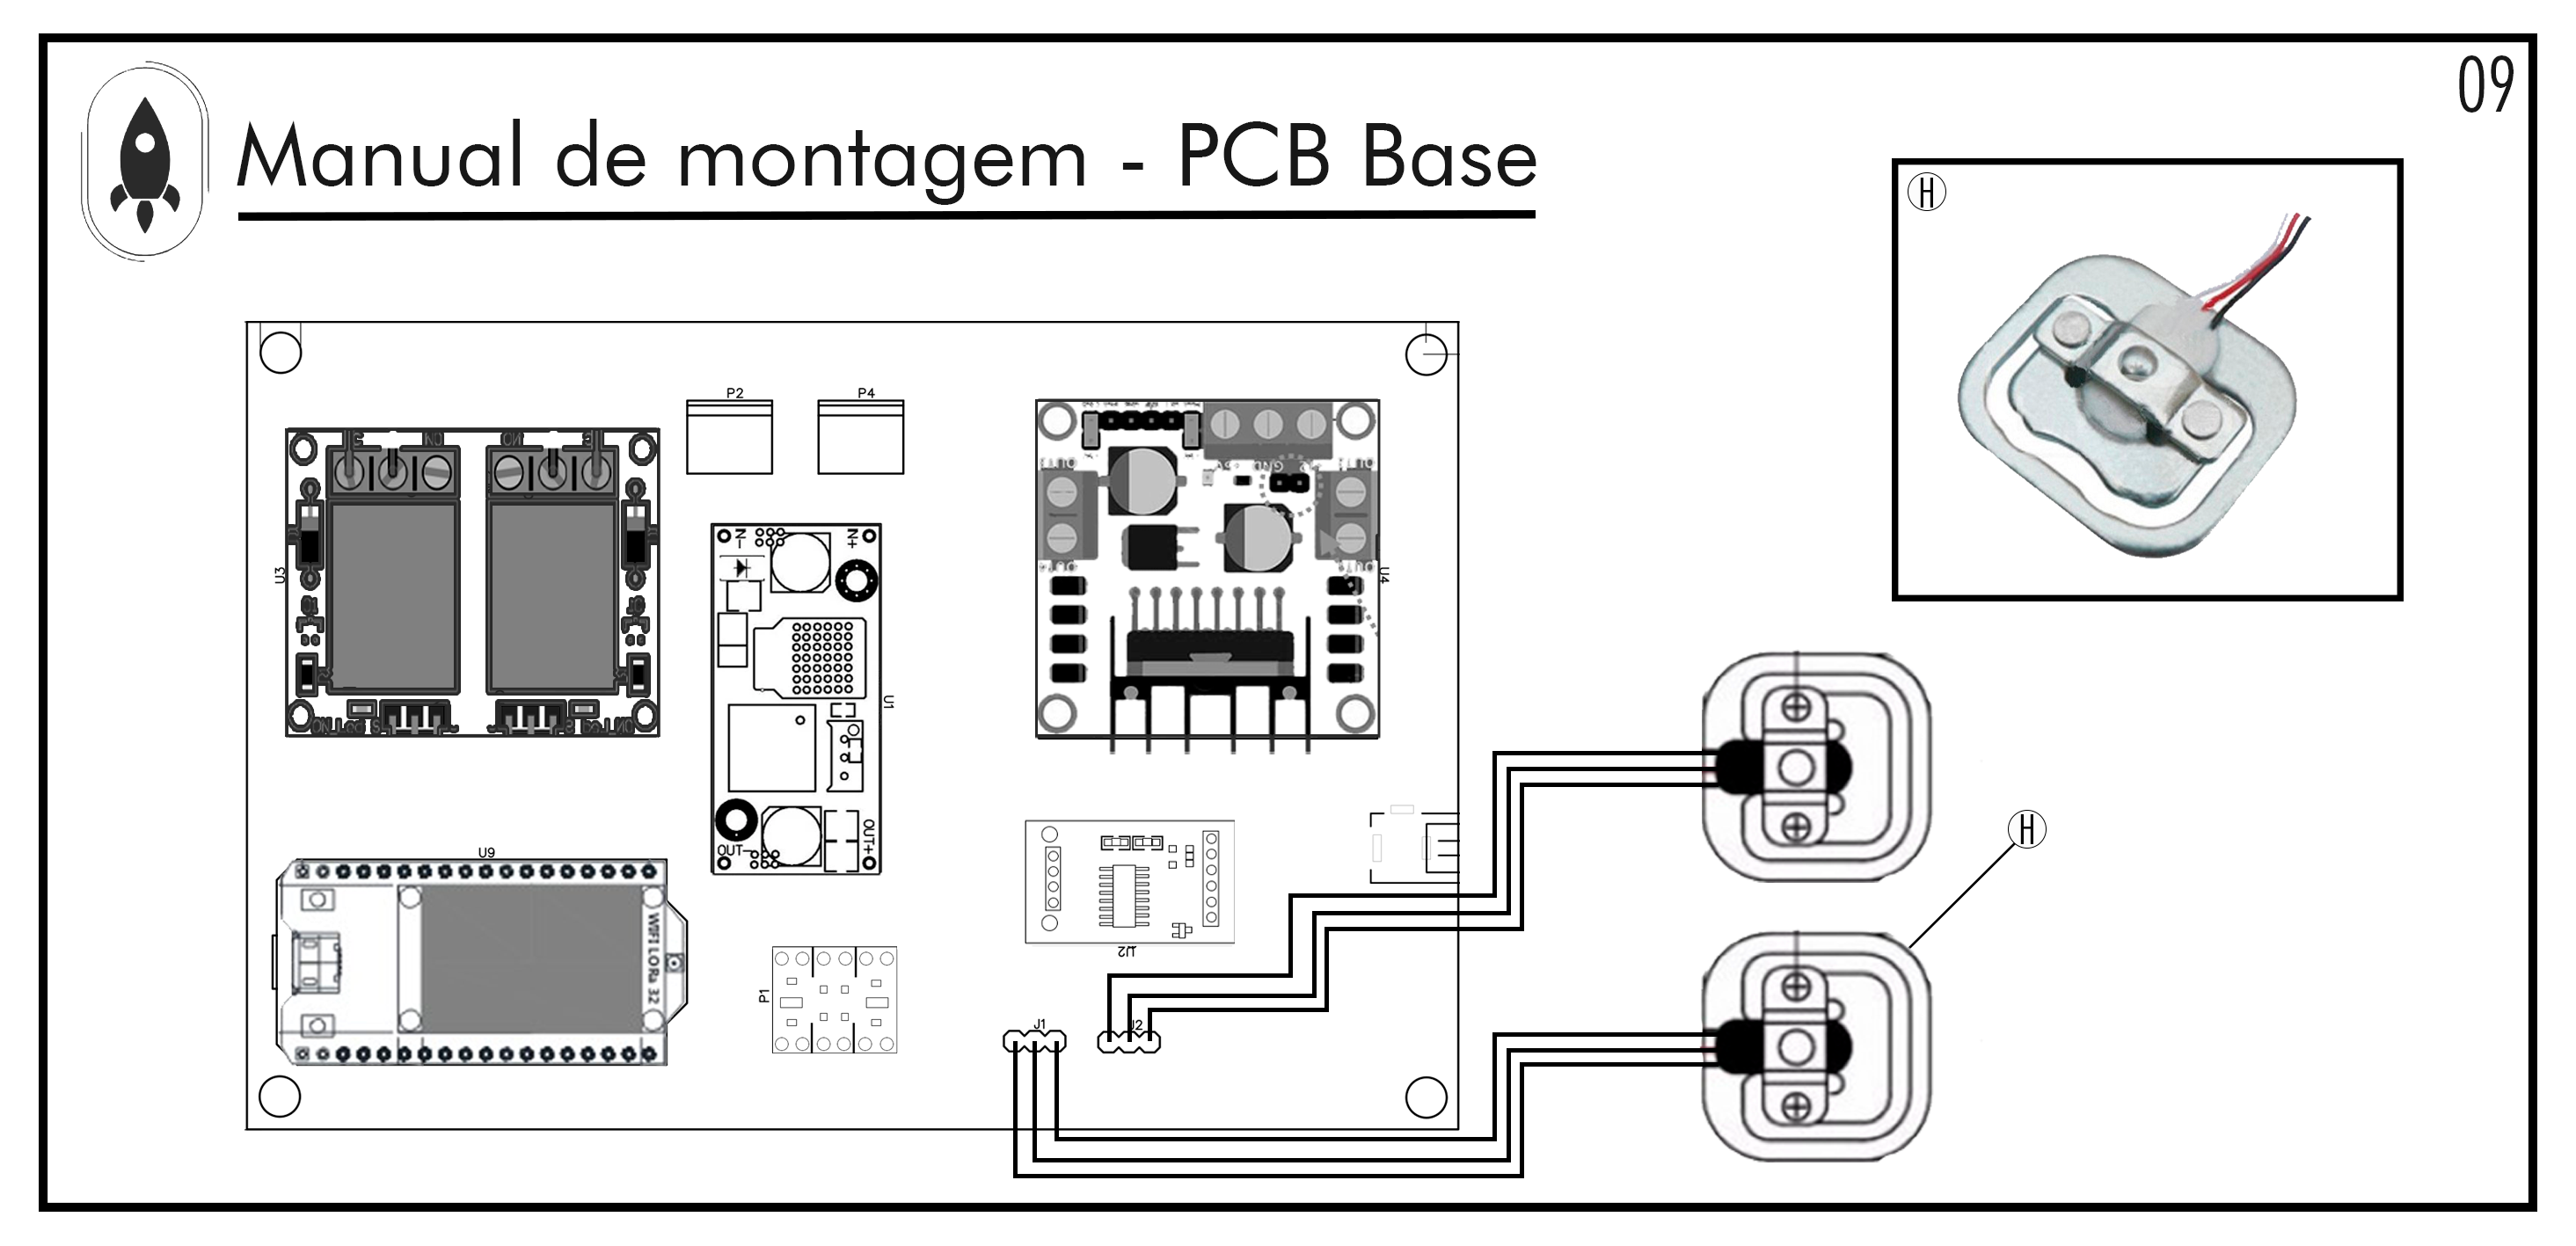
\includegraphics[width=\textwidth]{Figuras/BASE/Pg-09---PL-03.png}
  \caption{Sensor de Peso 50Kg Célula de Carga.}
 %{ \footnotesize Fonte: Autores} 
  \label{fig:PCIBASE Sensor de Peso 50Kg Célula de Carga  }
\end{figure}

\par Pegue o componente 'I'(Conector fêmea Jack P4 2,5mm), encaixe-a na posição mostrada \ref{fig:PCIBASE  Conector Jack P4 2,5mm    }   e solde junto a placa.
\begin{figure}[H]
  \centering
  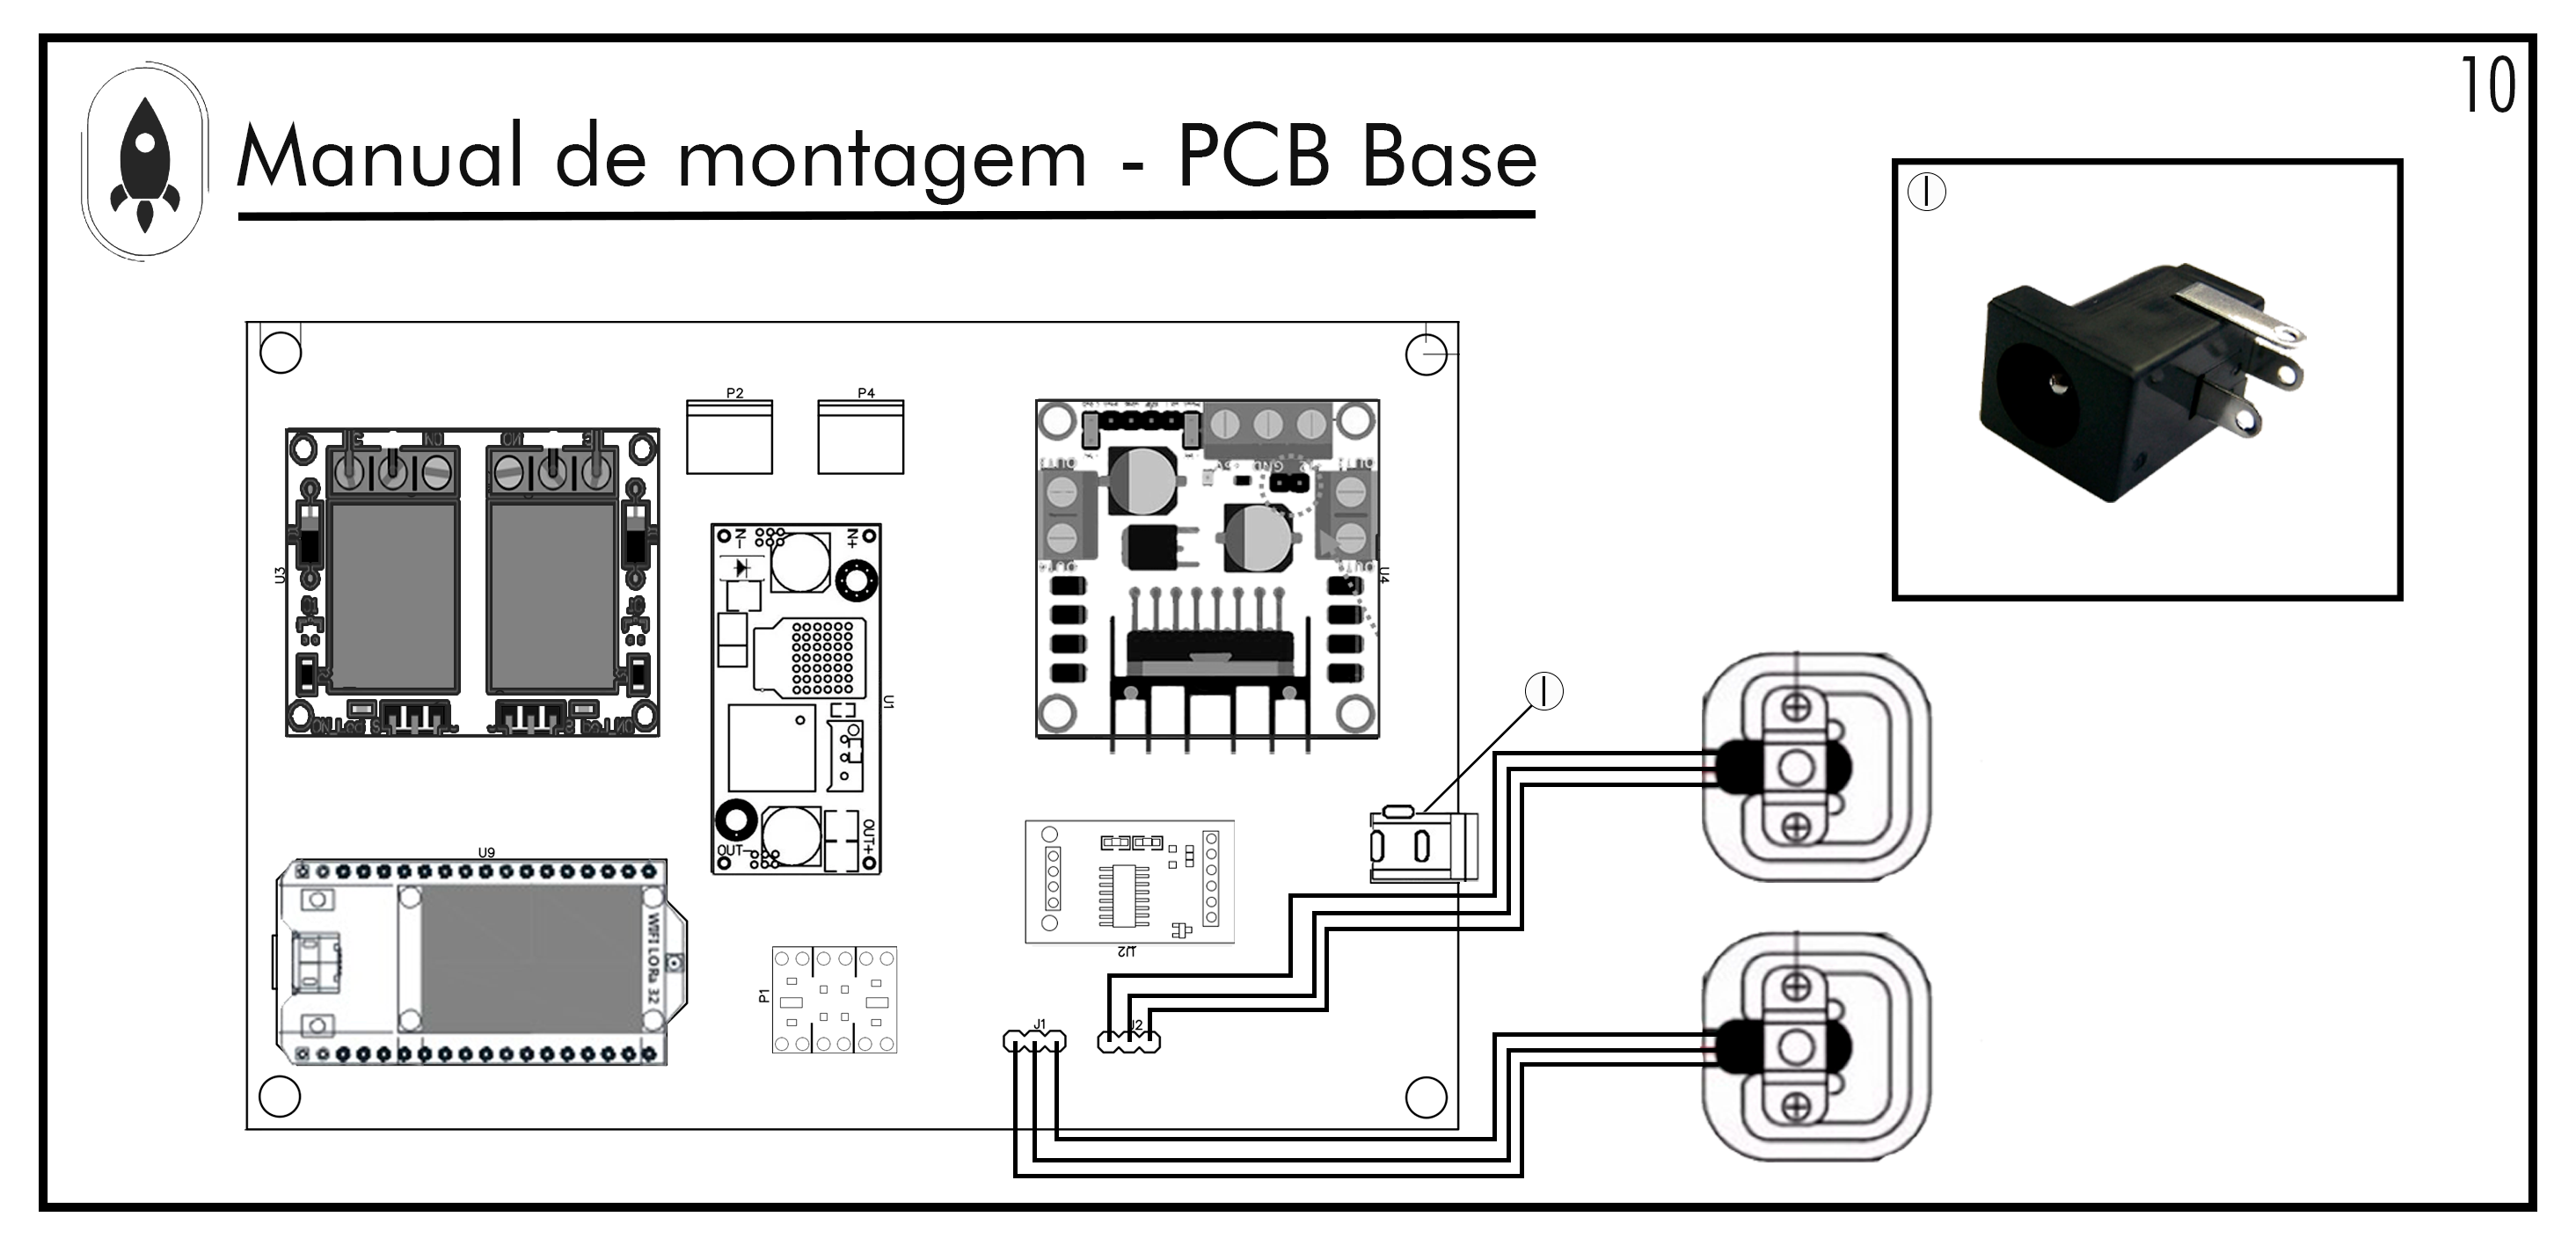
\includegraphics[width=\textwidth]{Figuras/BASE/Pg-10---PL-03.png}
  \caption{ Conector fêmea Jack P4 2,5mm.}
 %{ \footnotesize Fonte: Autores} 
  \label{fig:PCIBASE  Conector Jack P4 2,5mm  }
\end{figure}

\newpage
\par Pegue o componente 'J'(Borne Conector Kre 2 Vias), encaixe-a na posição mostrada \ref{fig:PCIBASE Borne Conector Kre 2 Vias }   e solde junto a placa.
\begin{figure}[H]
  \centering
  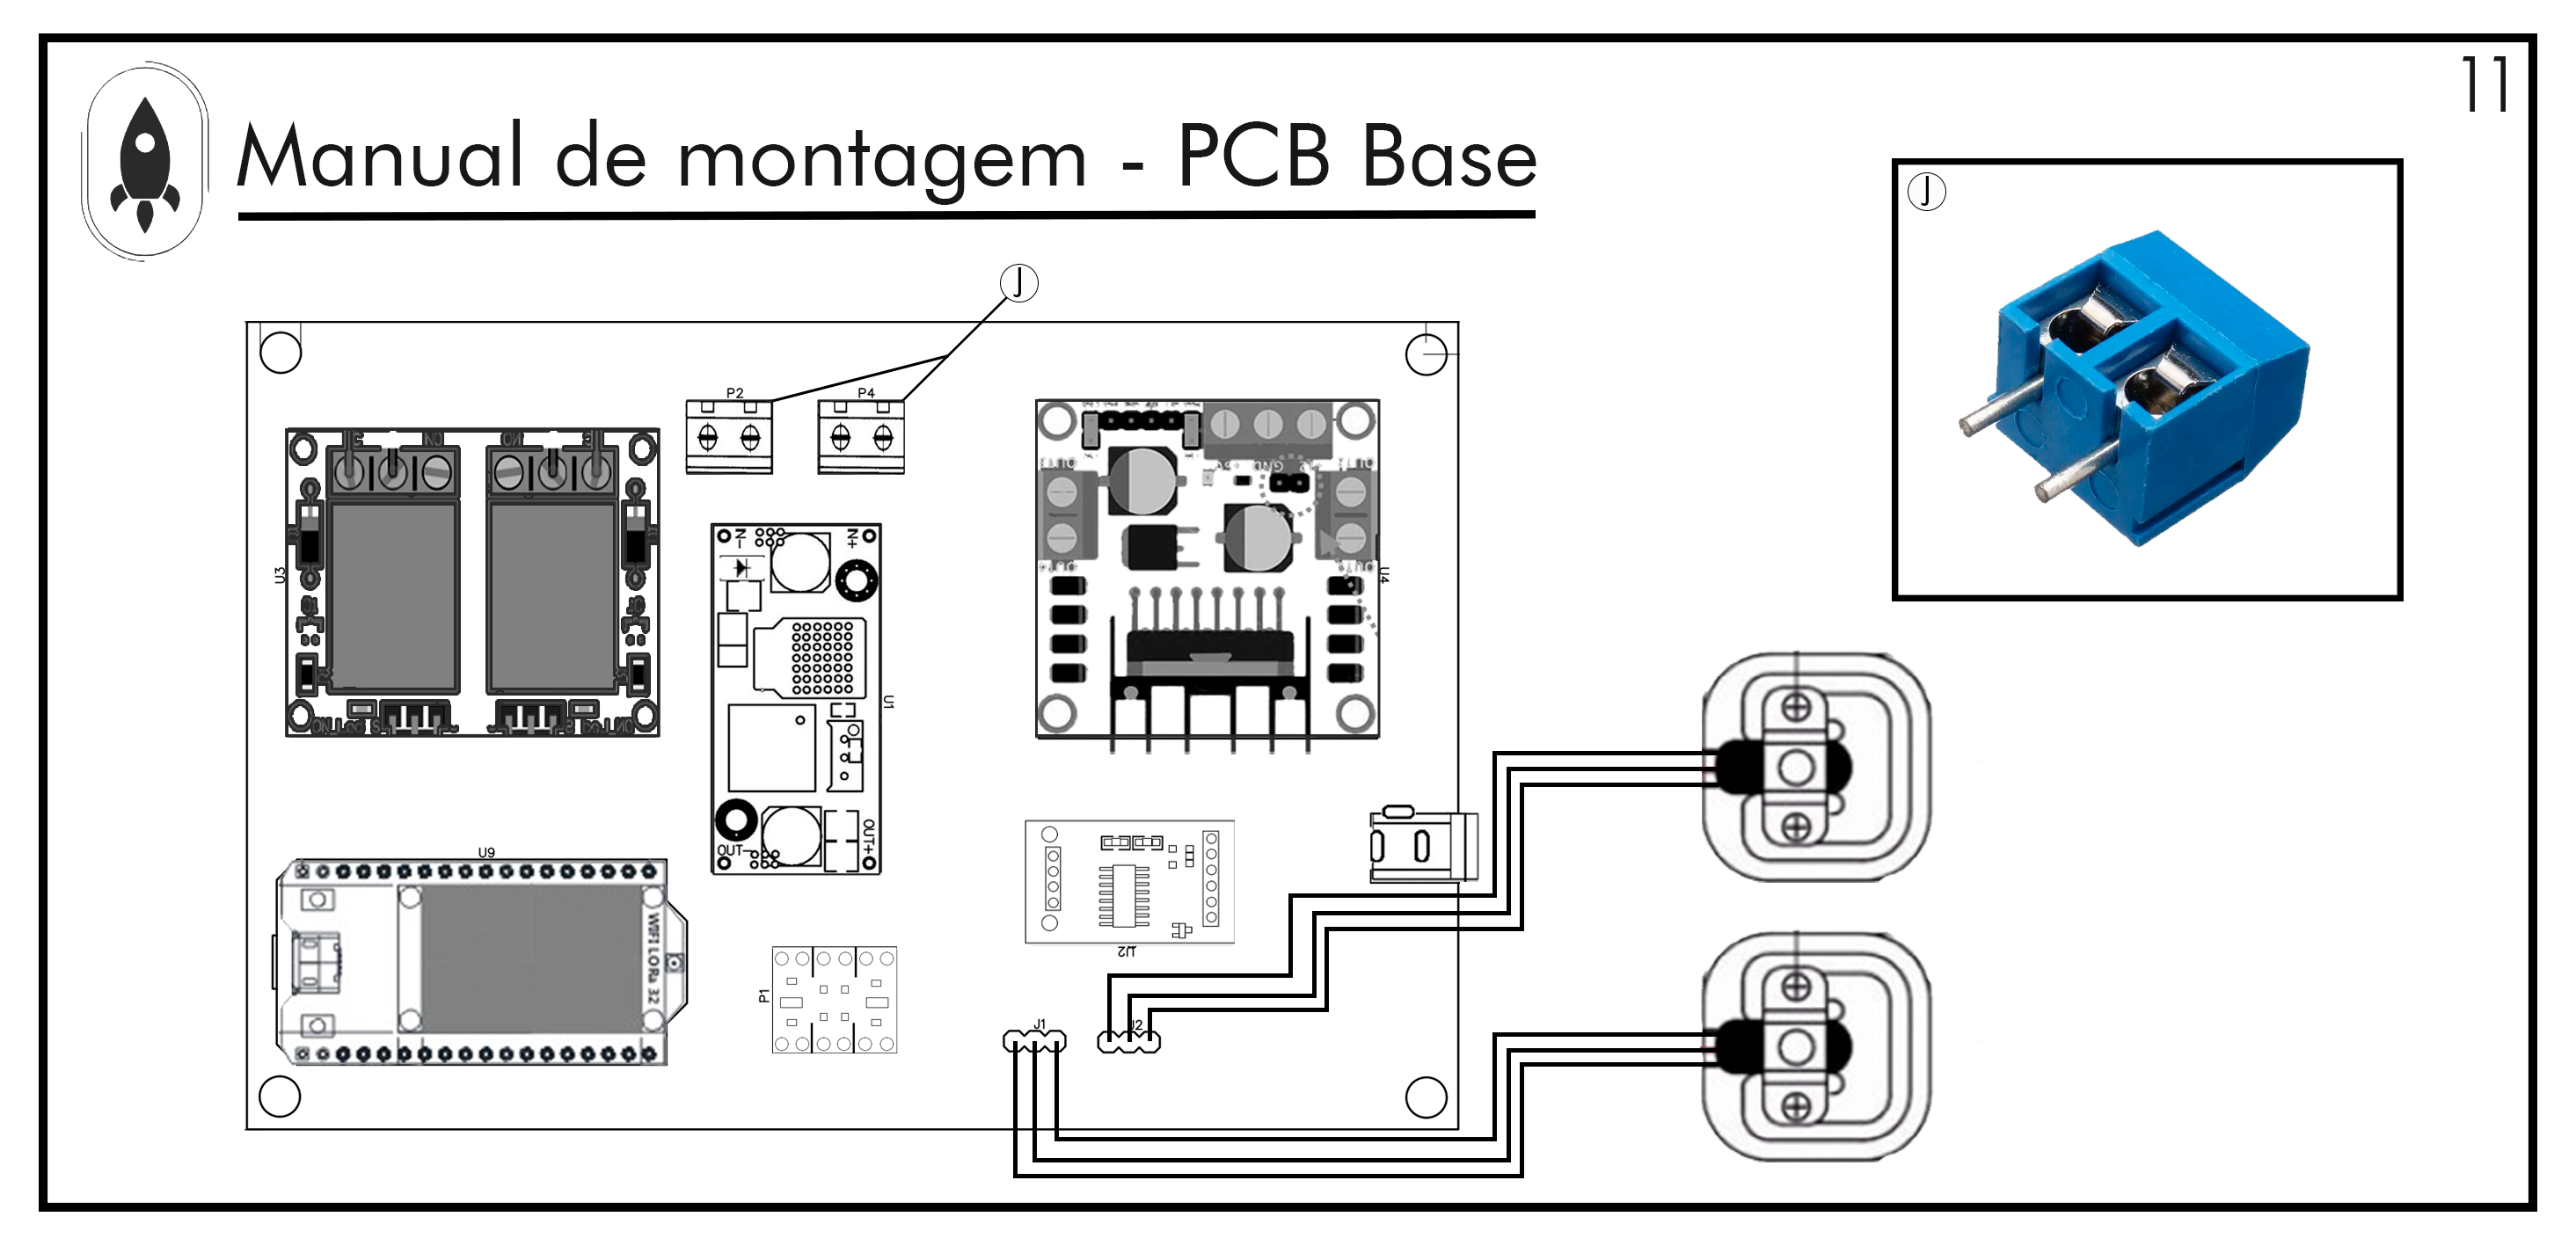
\includegraphics[width=\textwidth]{Figuras/BASE/Pg-11---PL-03.png}
  \caption{Borne Conector Kre 2 Vias.}
 %{ \footnotesize Fonte: Autores} 
  \label{fig:PCIBASE Borne Conector Kre 2 Vias  }
\end{figure}

\par Para a fixação da placa em seu recipiente utilize os parafusos e a porca extensora, componentes 'K' e 'L' e siga as instruções da seção \ref{sec:fixação }.

\subsection{Placas de Circuito Impresso-Foguete}

\subsubsection{Lista de Materiais}

\par Primeiramente é necessário ter em mão todos os componentes para sua montagem \ref{fig:Lista de materiais foguete}.

\begin{table}[H]
\centering
\begin{tabular}{|m{1.9cm} |m{1.8cm} |m{7.3cm}|m{4cm}|}
\hline
\begin{center}Identificador\end{center} &\begin{center} Quantidade\end{center} & \begin{center}Componente\end{center} &\begin{center} Part Number\end{center} \\\hline
A&01 &  PCI- Foguete  & -  \\\hline
B &01&Lora Esp32 Sx1278 Com Display  Oled Wifi bluetooth 915mhz& Sx1278 \\\hline
 
C&01 &  Conversor DC-DC Step Down-LM2596 (12~5V)
& LM2596 \\\hline

D&01 & Conector Jack J4 DC Fêmea &  Jack Fêmea  \\\hline

E&01&Sensor De Pressão e Temperatura BMP 280 & BST-BMP280-DS001-11 \\\hline

F&01 &  Módulo Relé 5V 2 Canais &   SRD-05VDC-SL-C \\\hline

G &01 & Módulo Gps  Gy-gps6m v2 & GPS NEO6M \\\hline

H&01 & Módulo Cartão de Memória MICRO SD CARD & B01IPCAP72 \\\hline

I&01&Conector Borne KRE 2 Vias & KRE Kf301 \\\hline

J&05&Parafuso Máquina Cabeça Chata Phillips M5 X 20mm &  Phillips M5 X 20mm \\\hline

K&05& porca de bronze espaçador hexagonal M5 X 12mm & -  \\\hline

\end{tabular}
\caption{Lista de componentes}
\end{table}


\subsubsection{Instruções}


\begin{figure}[H]
  \centering
  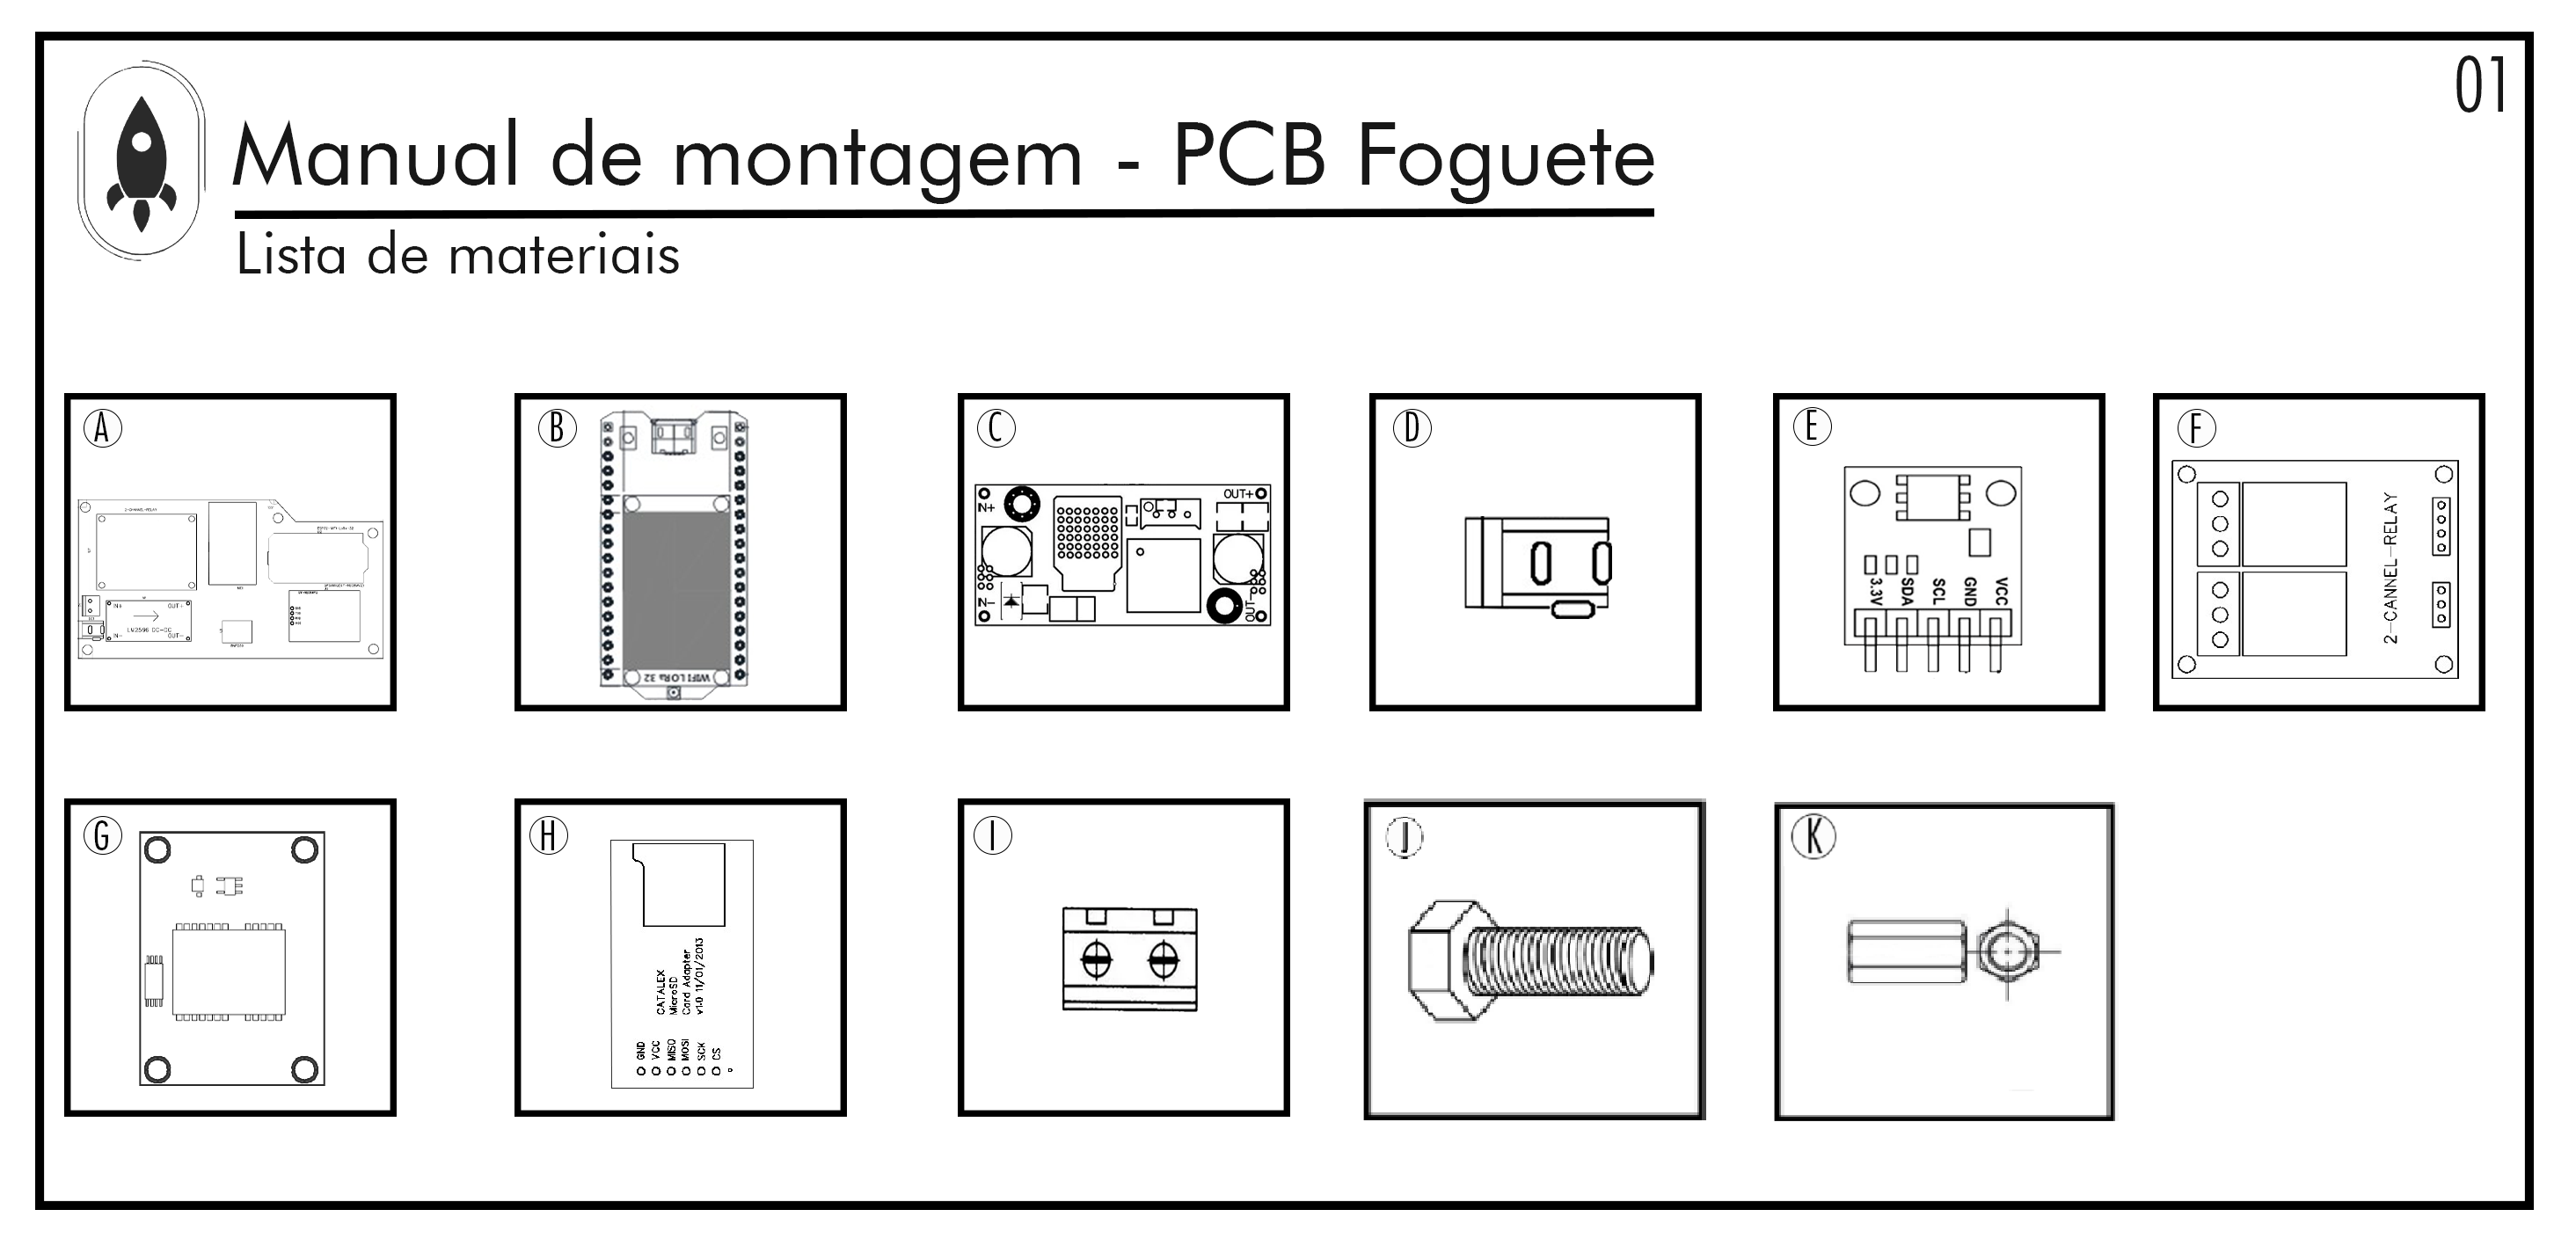
\includegraphics[width=\textwidth]{Figuras/FOGUETE/Pg-01---PL-02.png}
  \caption{Lista de Materiais.} 
 %{ \footnotesize Fonte: Autores} 
  \label{fig:Lista de materiais foguete}
\end{figure}



\par Com todos os componentes em mãos, pegue componente 'A'(PCI-Foguete) prepare-a para soldagem dos componentes passando uma fina camada de solda nos pads da PCI.

\begin{figure}[H]
  \centering
  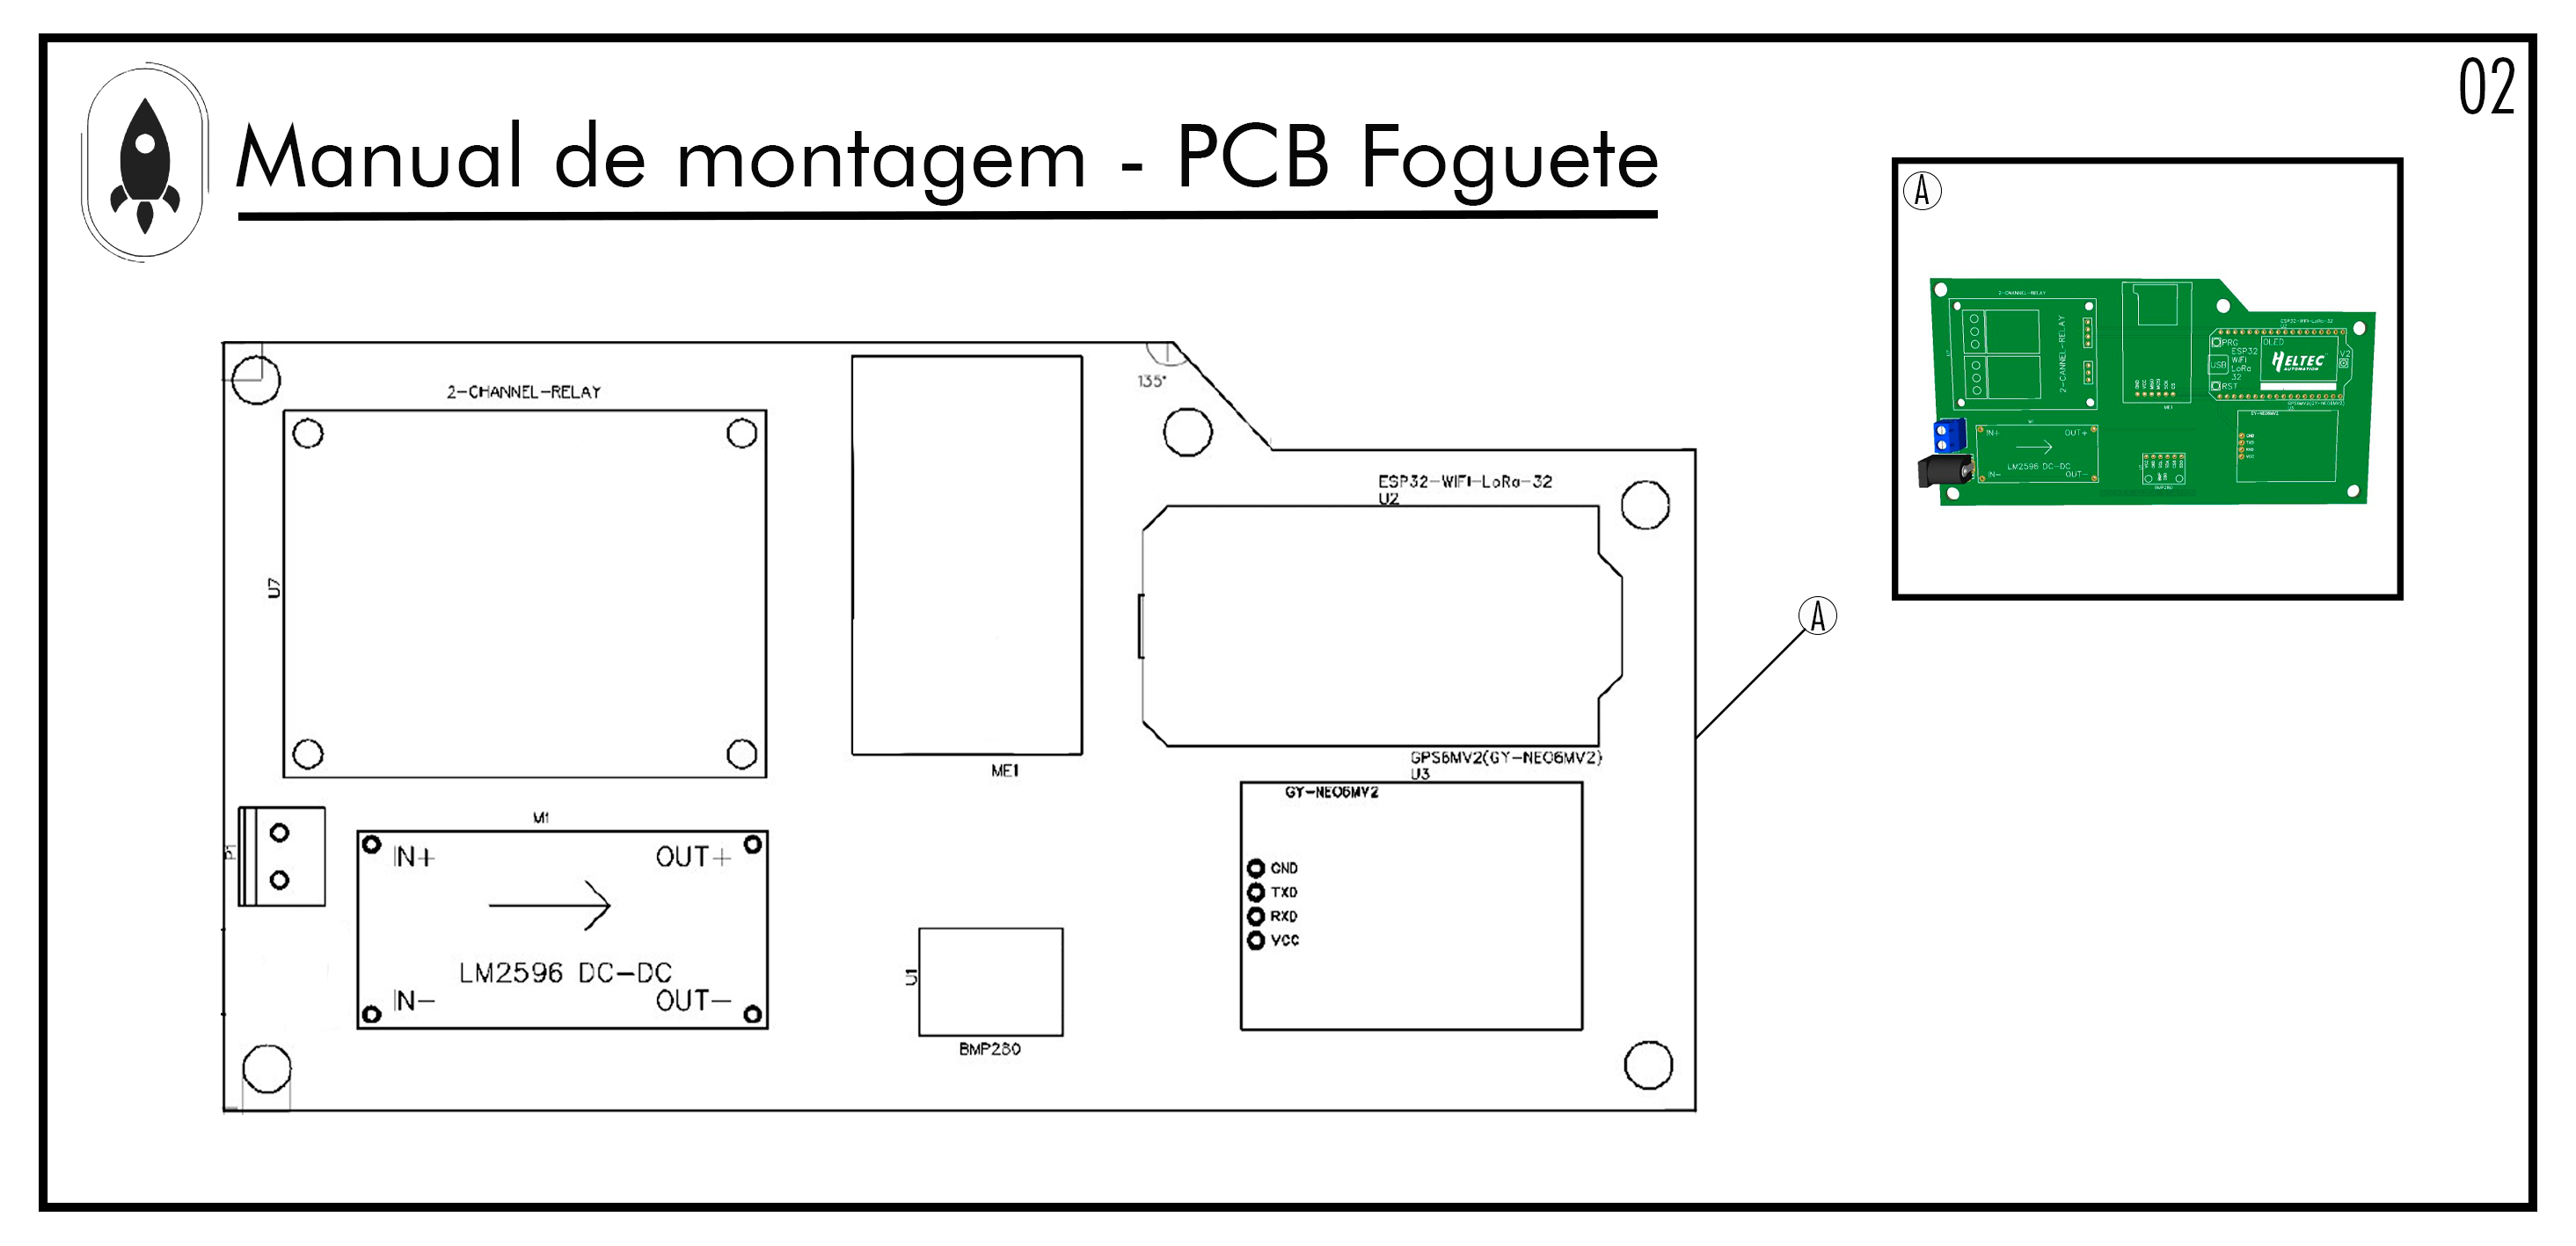
\includegraphics[width=\textwidth]{Figuras/FOGUETE/Pg-02---PL-02.png}
  \caption{PCI do foguete.}
 %{ \footnotesize Fonte: Autores} 
  \label{fig:PCIFoguete}
\end{figure}

\par Pegue o componente 'B'(ESP32 LoRa WiFi), encaixe-a na posição mostrada \ref{fig:PCIFoguete LORA} e solde junto a placa.
\begin{figure}[H]
  \centering
  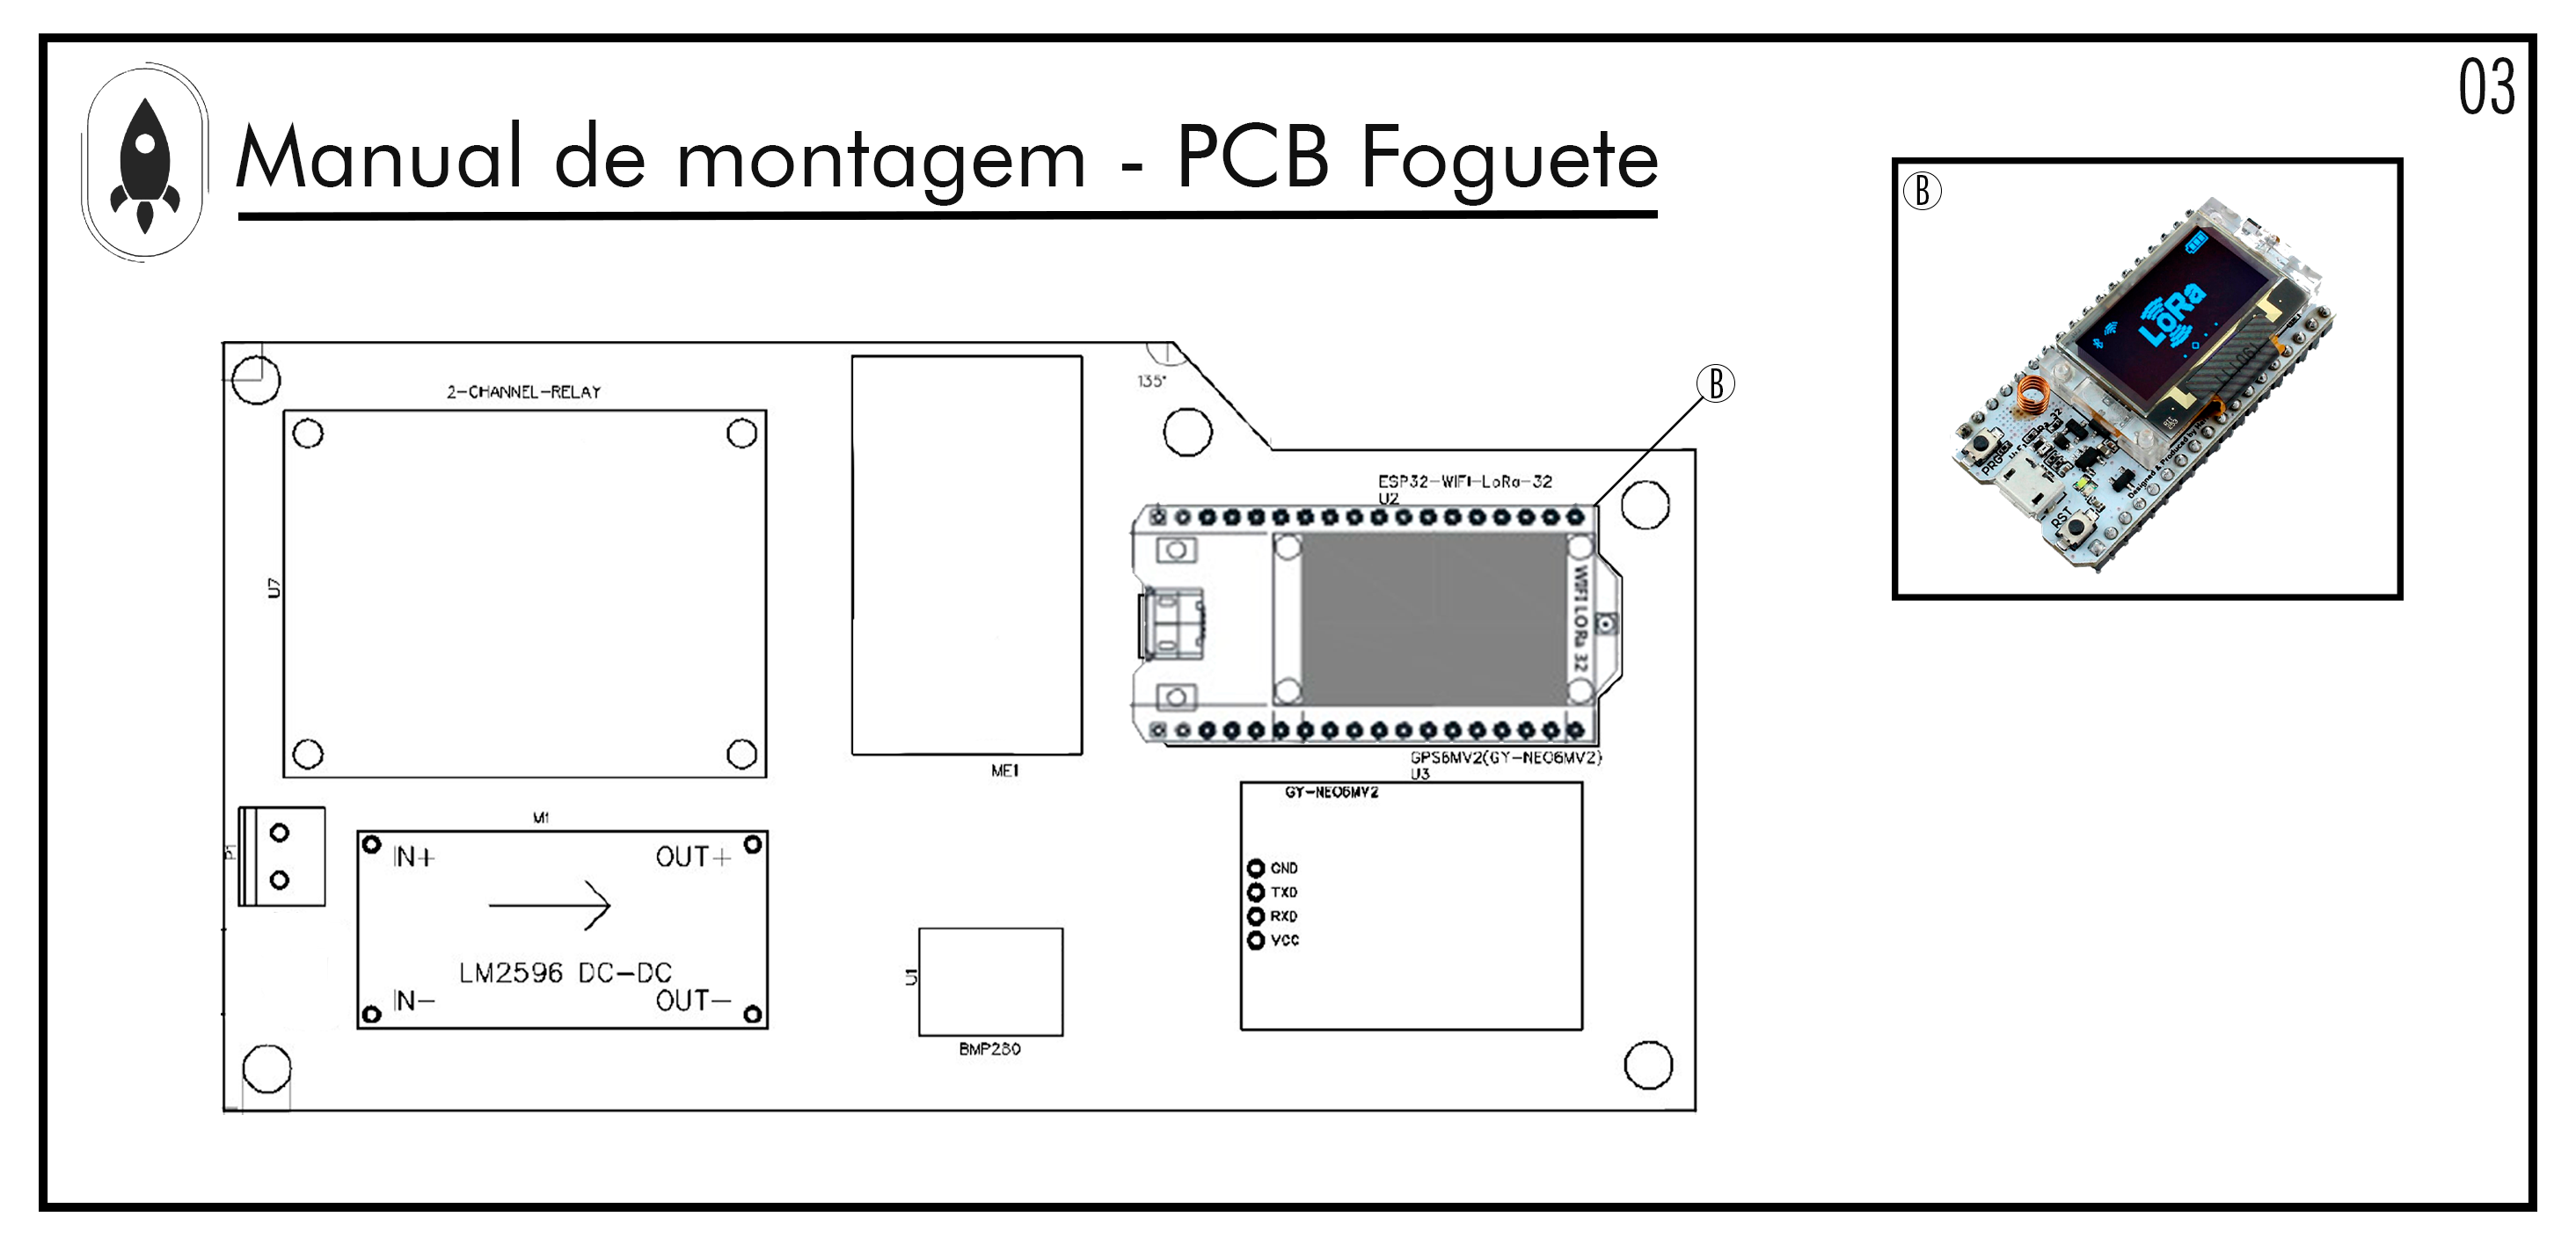
\includegraphics[width=\textwidth]{Figuras/FOGUETE/Pg-03---PL-02.png}
  \caption{ESP32 WiFi Lora.}
 %{ \footnotesize Fonte: Autores} 
  \label{fig:PCIFoguete LORA}
\end{figure}

\newpage

\par Pegue o componente 'C'(LM2596), encaixe-a na posição mostrada \ref{fig:PCIFoguete LM2596} e solde junto  a placa.
\begin{figure}[H]
  \centering
  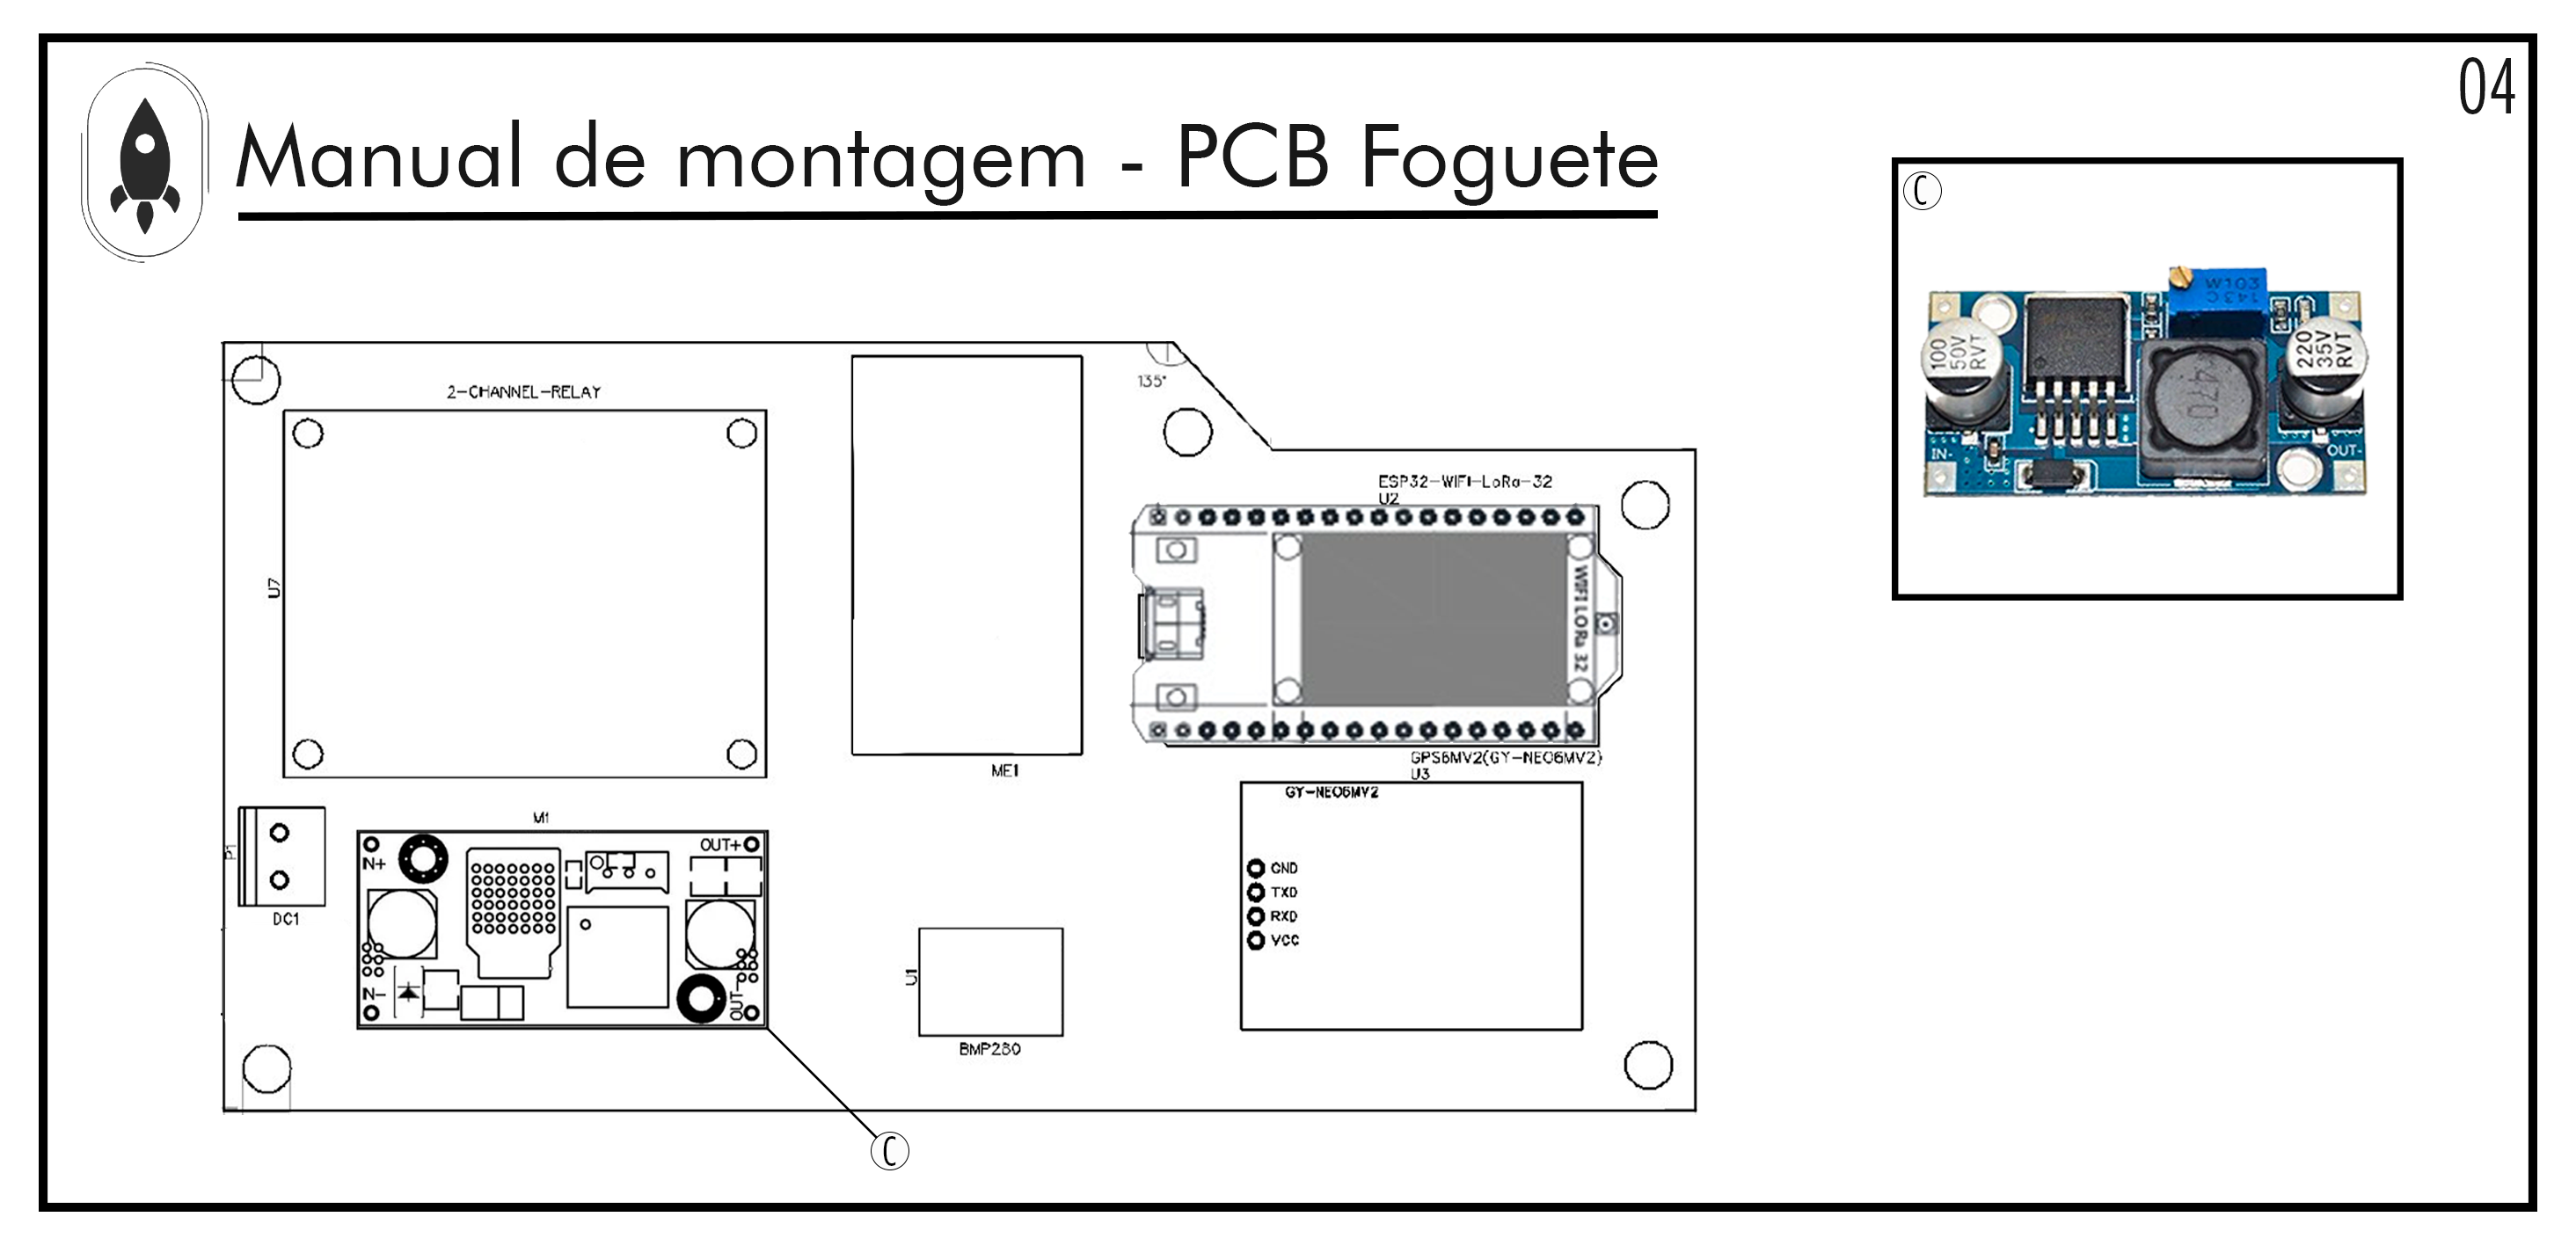
\includegraphics[width=\textwidth]{Figuras/FOGUETE/Pg-04---PL-02.png}
  \caption{LM2596.}
 %{ \footnotesize Fonte: Autores} 
  \label{fig:PCIFoguete LM2596}
\end{figure}


\par Pegue o componente 'D'(Conector fêmea jack P4 2,5mm), encaixe-a na posição mostrada \ref{fig:PCIFoguete jack P4} e solde junto a placa.
\begin{figure}[H]
  \centering
  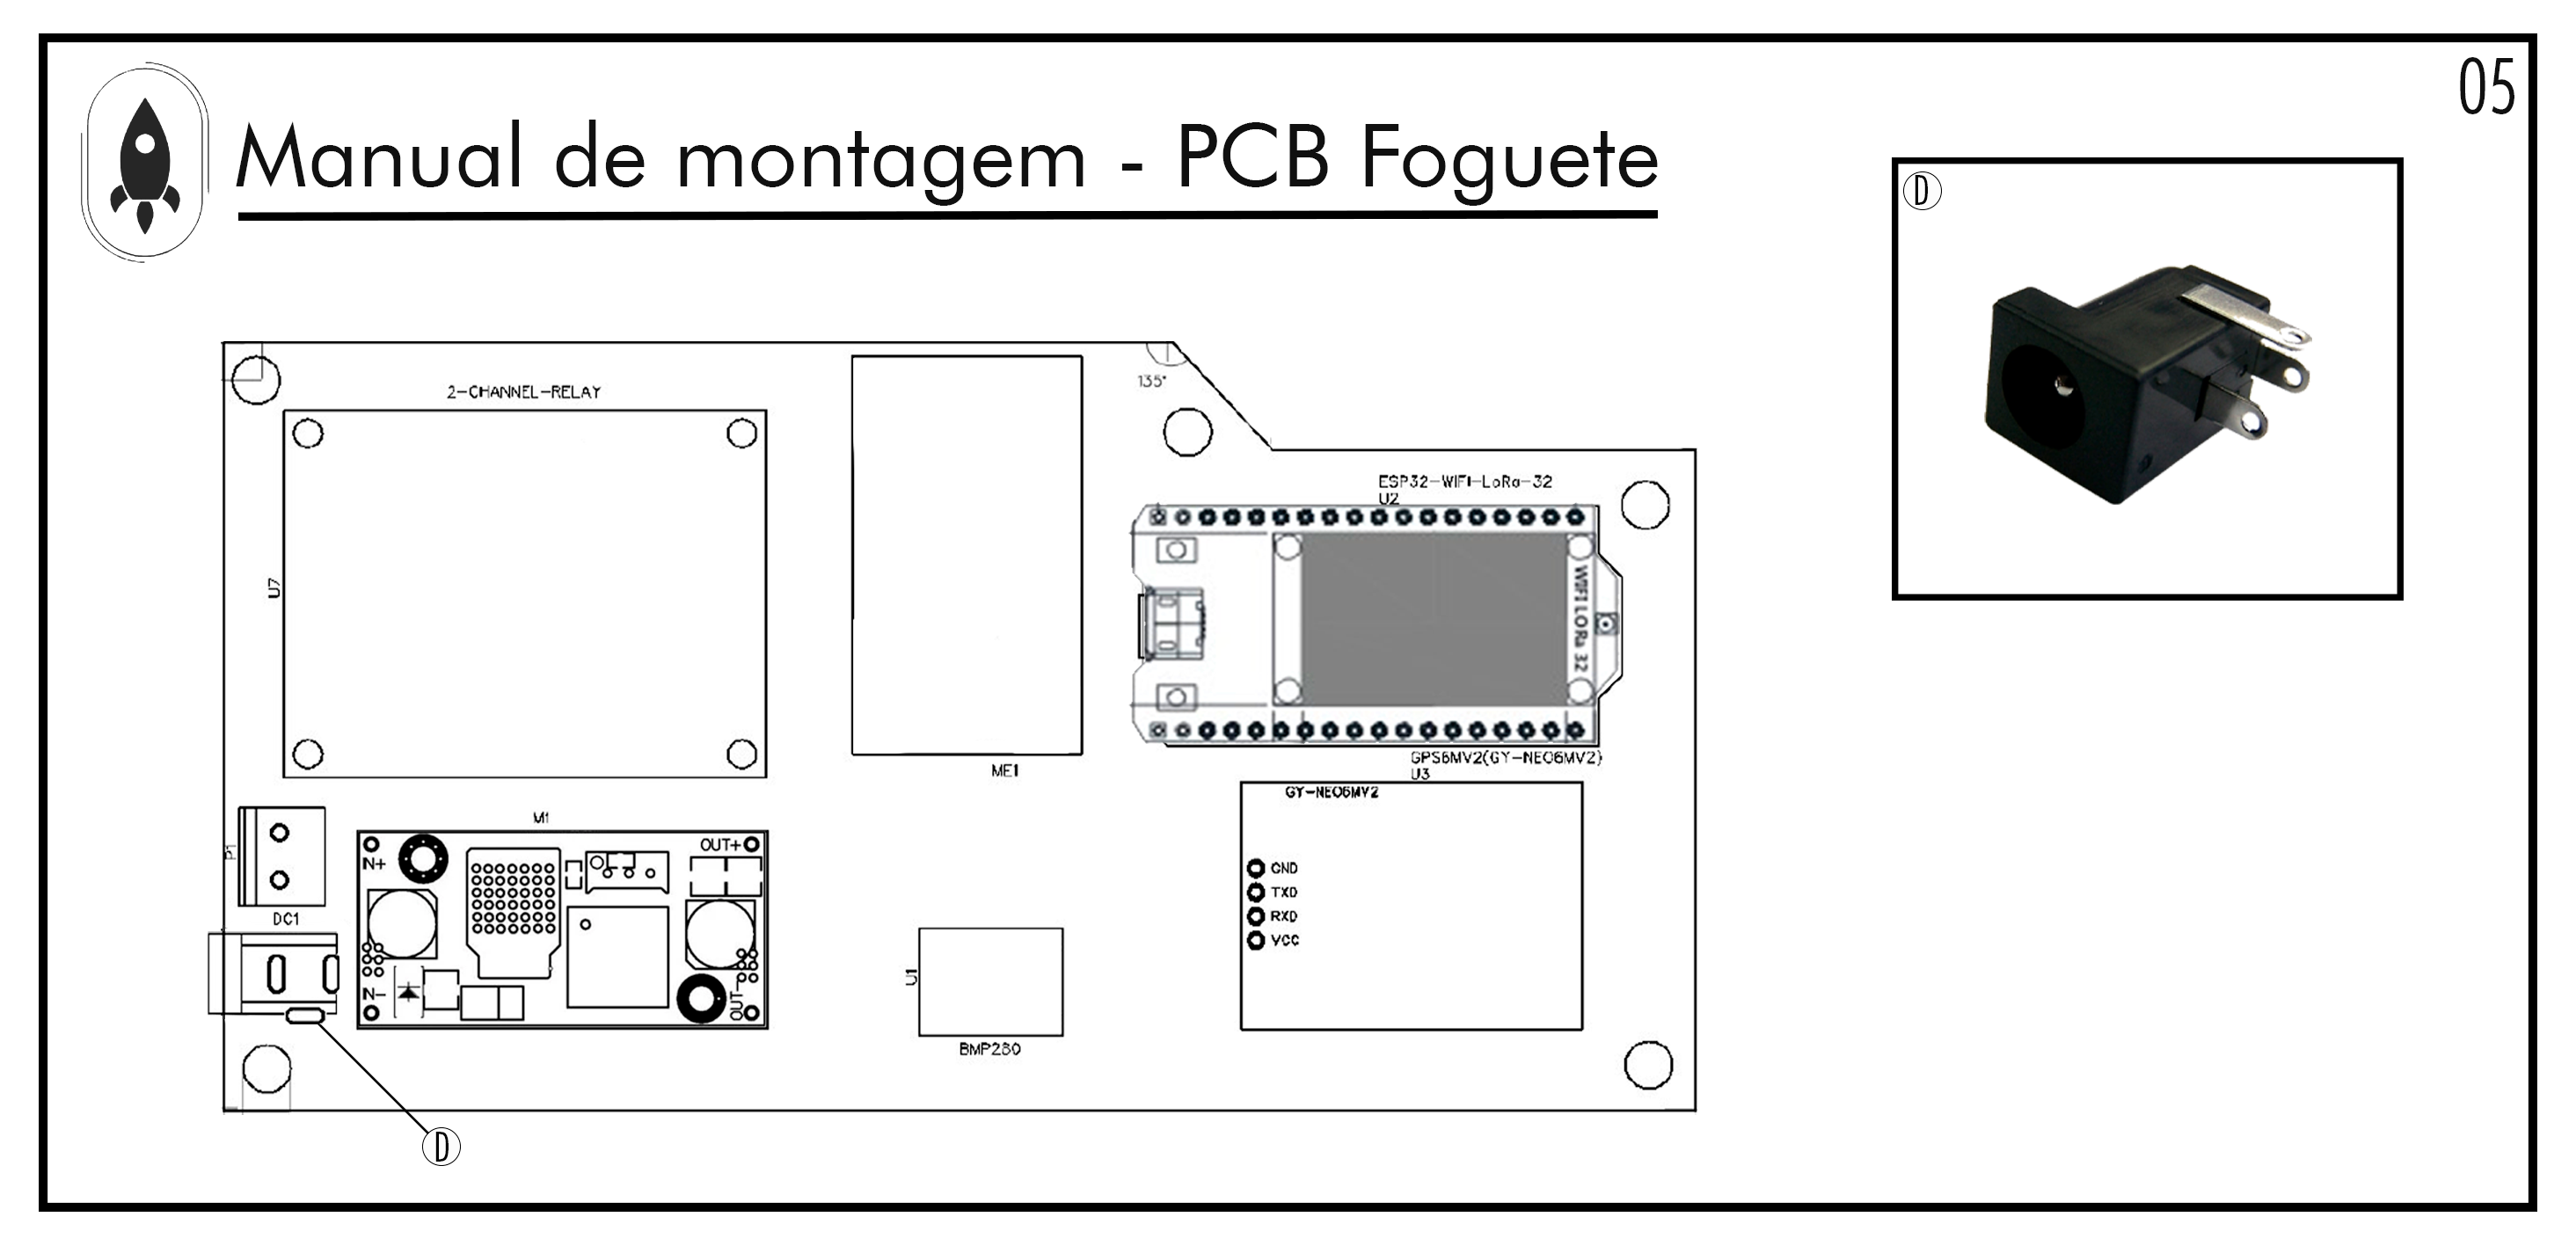
\includegraphics[width=\textwidth]{Figuras/FOGUETE/Pg-05---PL-02.png}
  \caption{Conector fêmea jack P4 2,5mm.}
 %{ \footnotesize Fonte: Autores} 
  \label{fig:PCIFoguete jack P4}
\end{figure}

\newpage

\par Pegue o componente 'E'(Sensor de Pressão e temperatura BMP280), encaixe-a na posição mostrada \ref{fig:PCIFoguete BMP280} e solde junto a placa.
\begin{figure}[H]
  \centering
  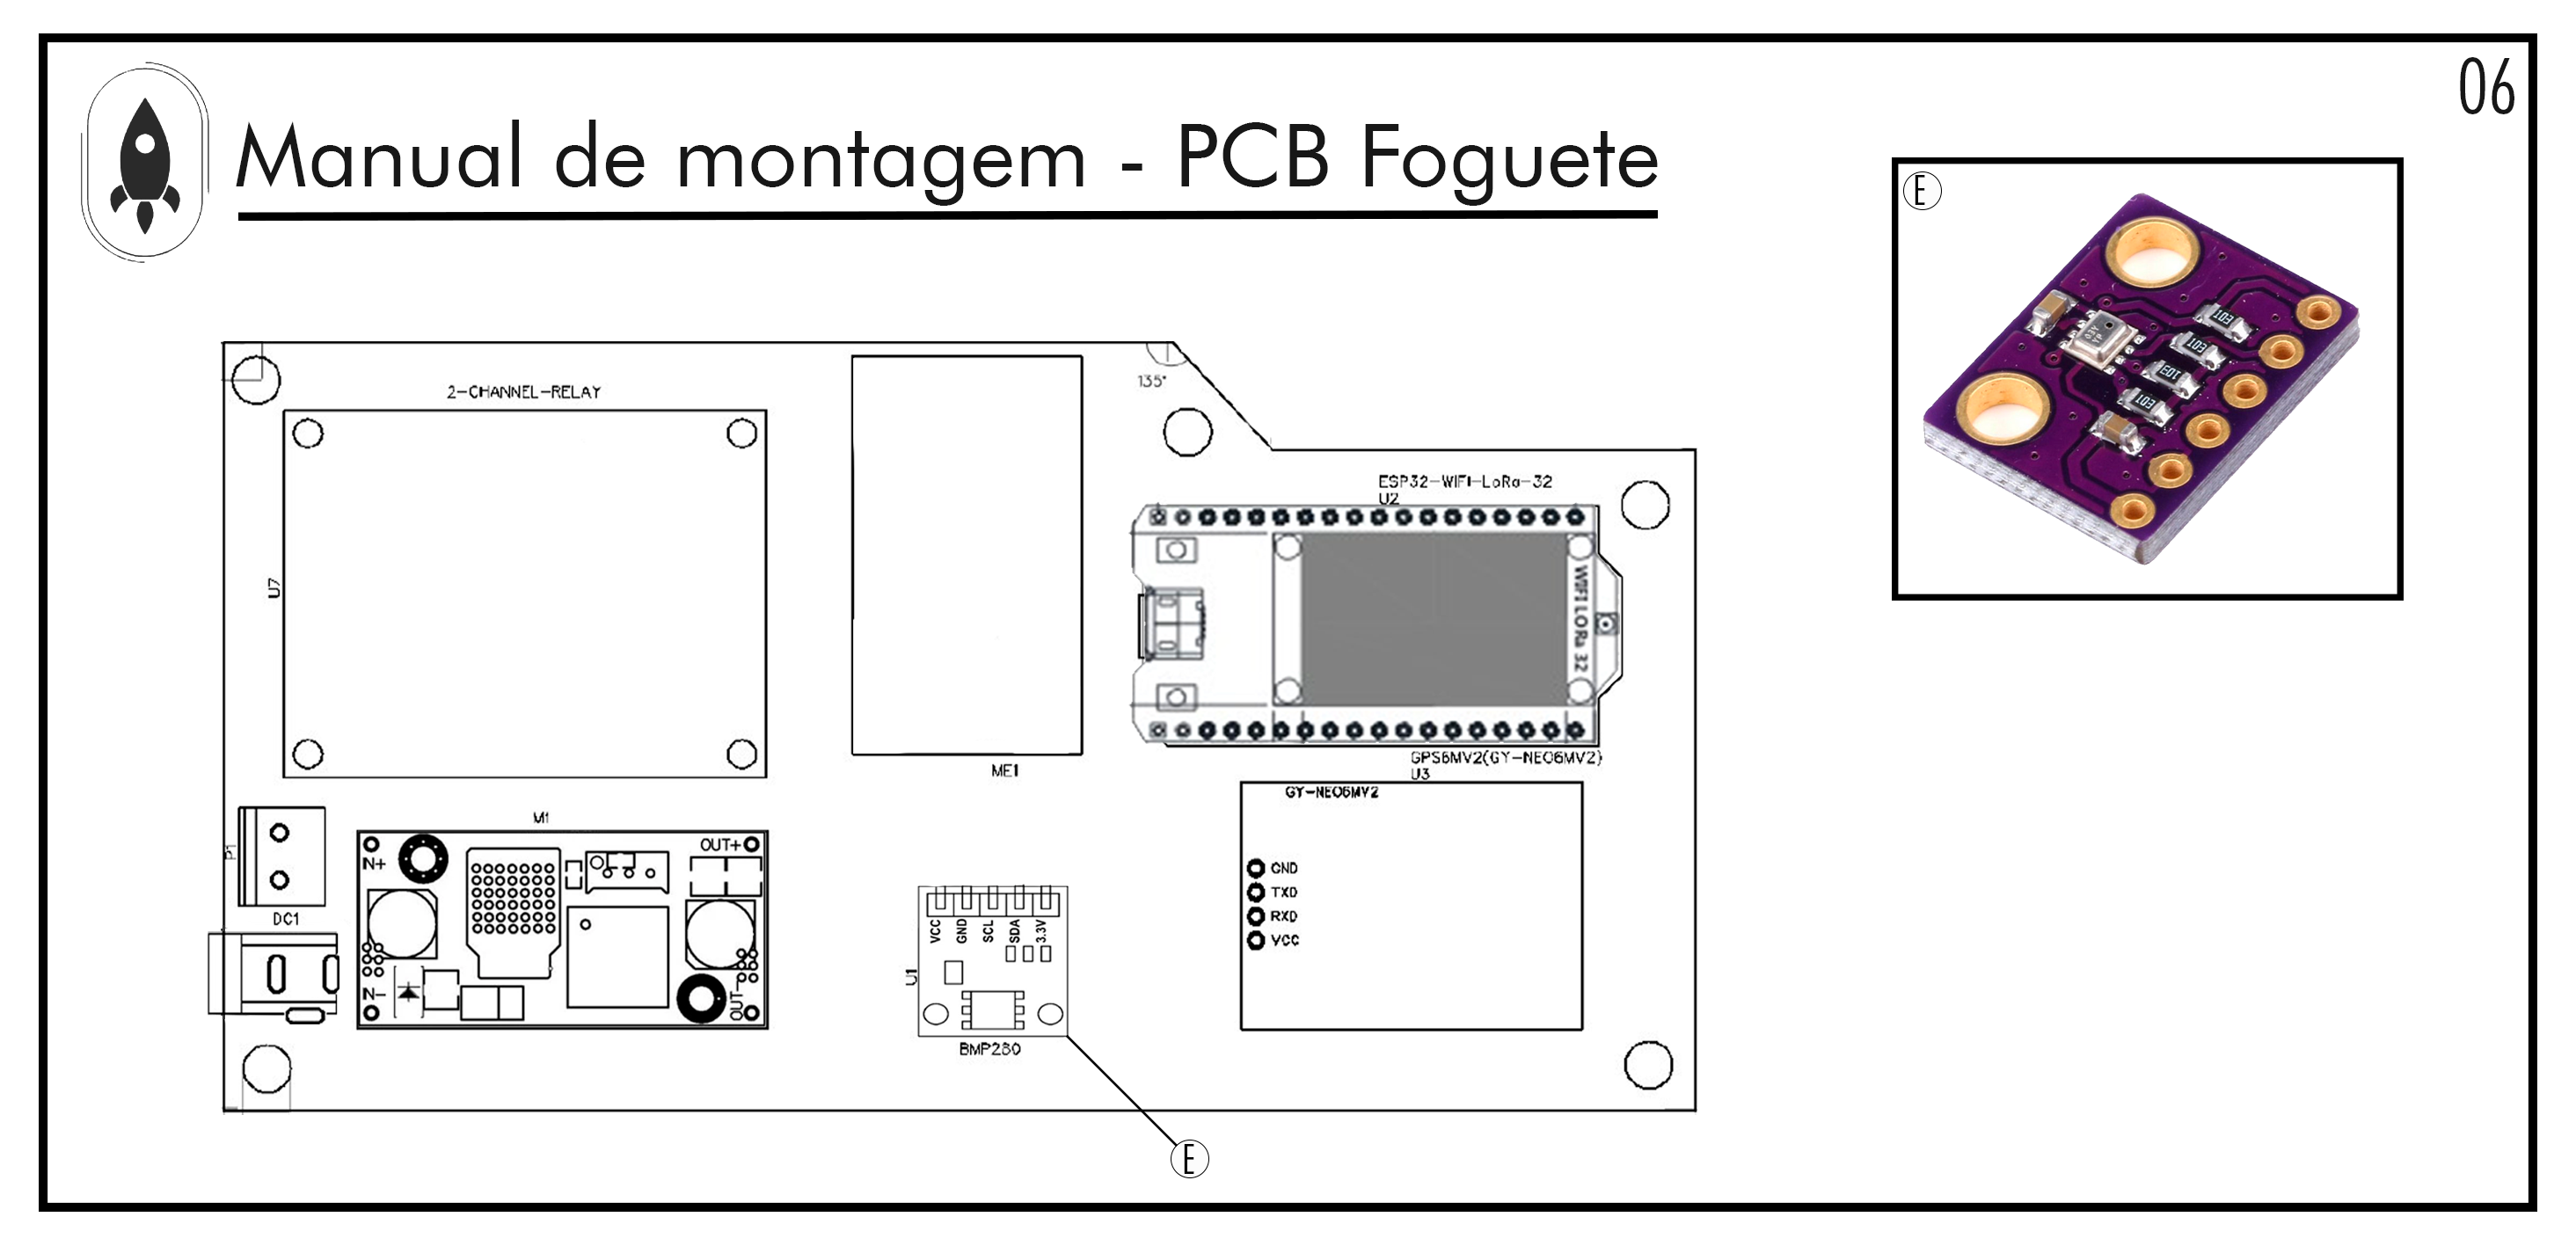
\includegraphics[width=\textwidth]{Figuras/FOGUETE/Pg-06---PL-02.png}
  \caption{Sensor de Pressão e temperatura BMP280.}
 %{ \footnotesize Fonte: Autores} 
  \label{fig:PCIFoguete BMP280}
\end{figure}


\par Pegue o componente 'F'(Módulo Relé 5V 2 Canais modelo SRD-05VDC-SL-C), encaixe-a na posição mostrada \ref{fig:PCIFoguete Relé} e solde junto  a placa.
\begin{figure}[H]
  \centering
  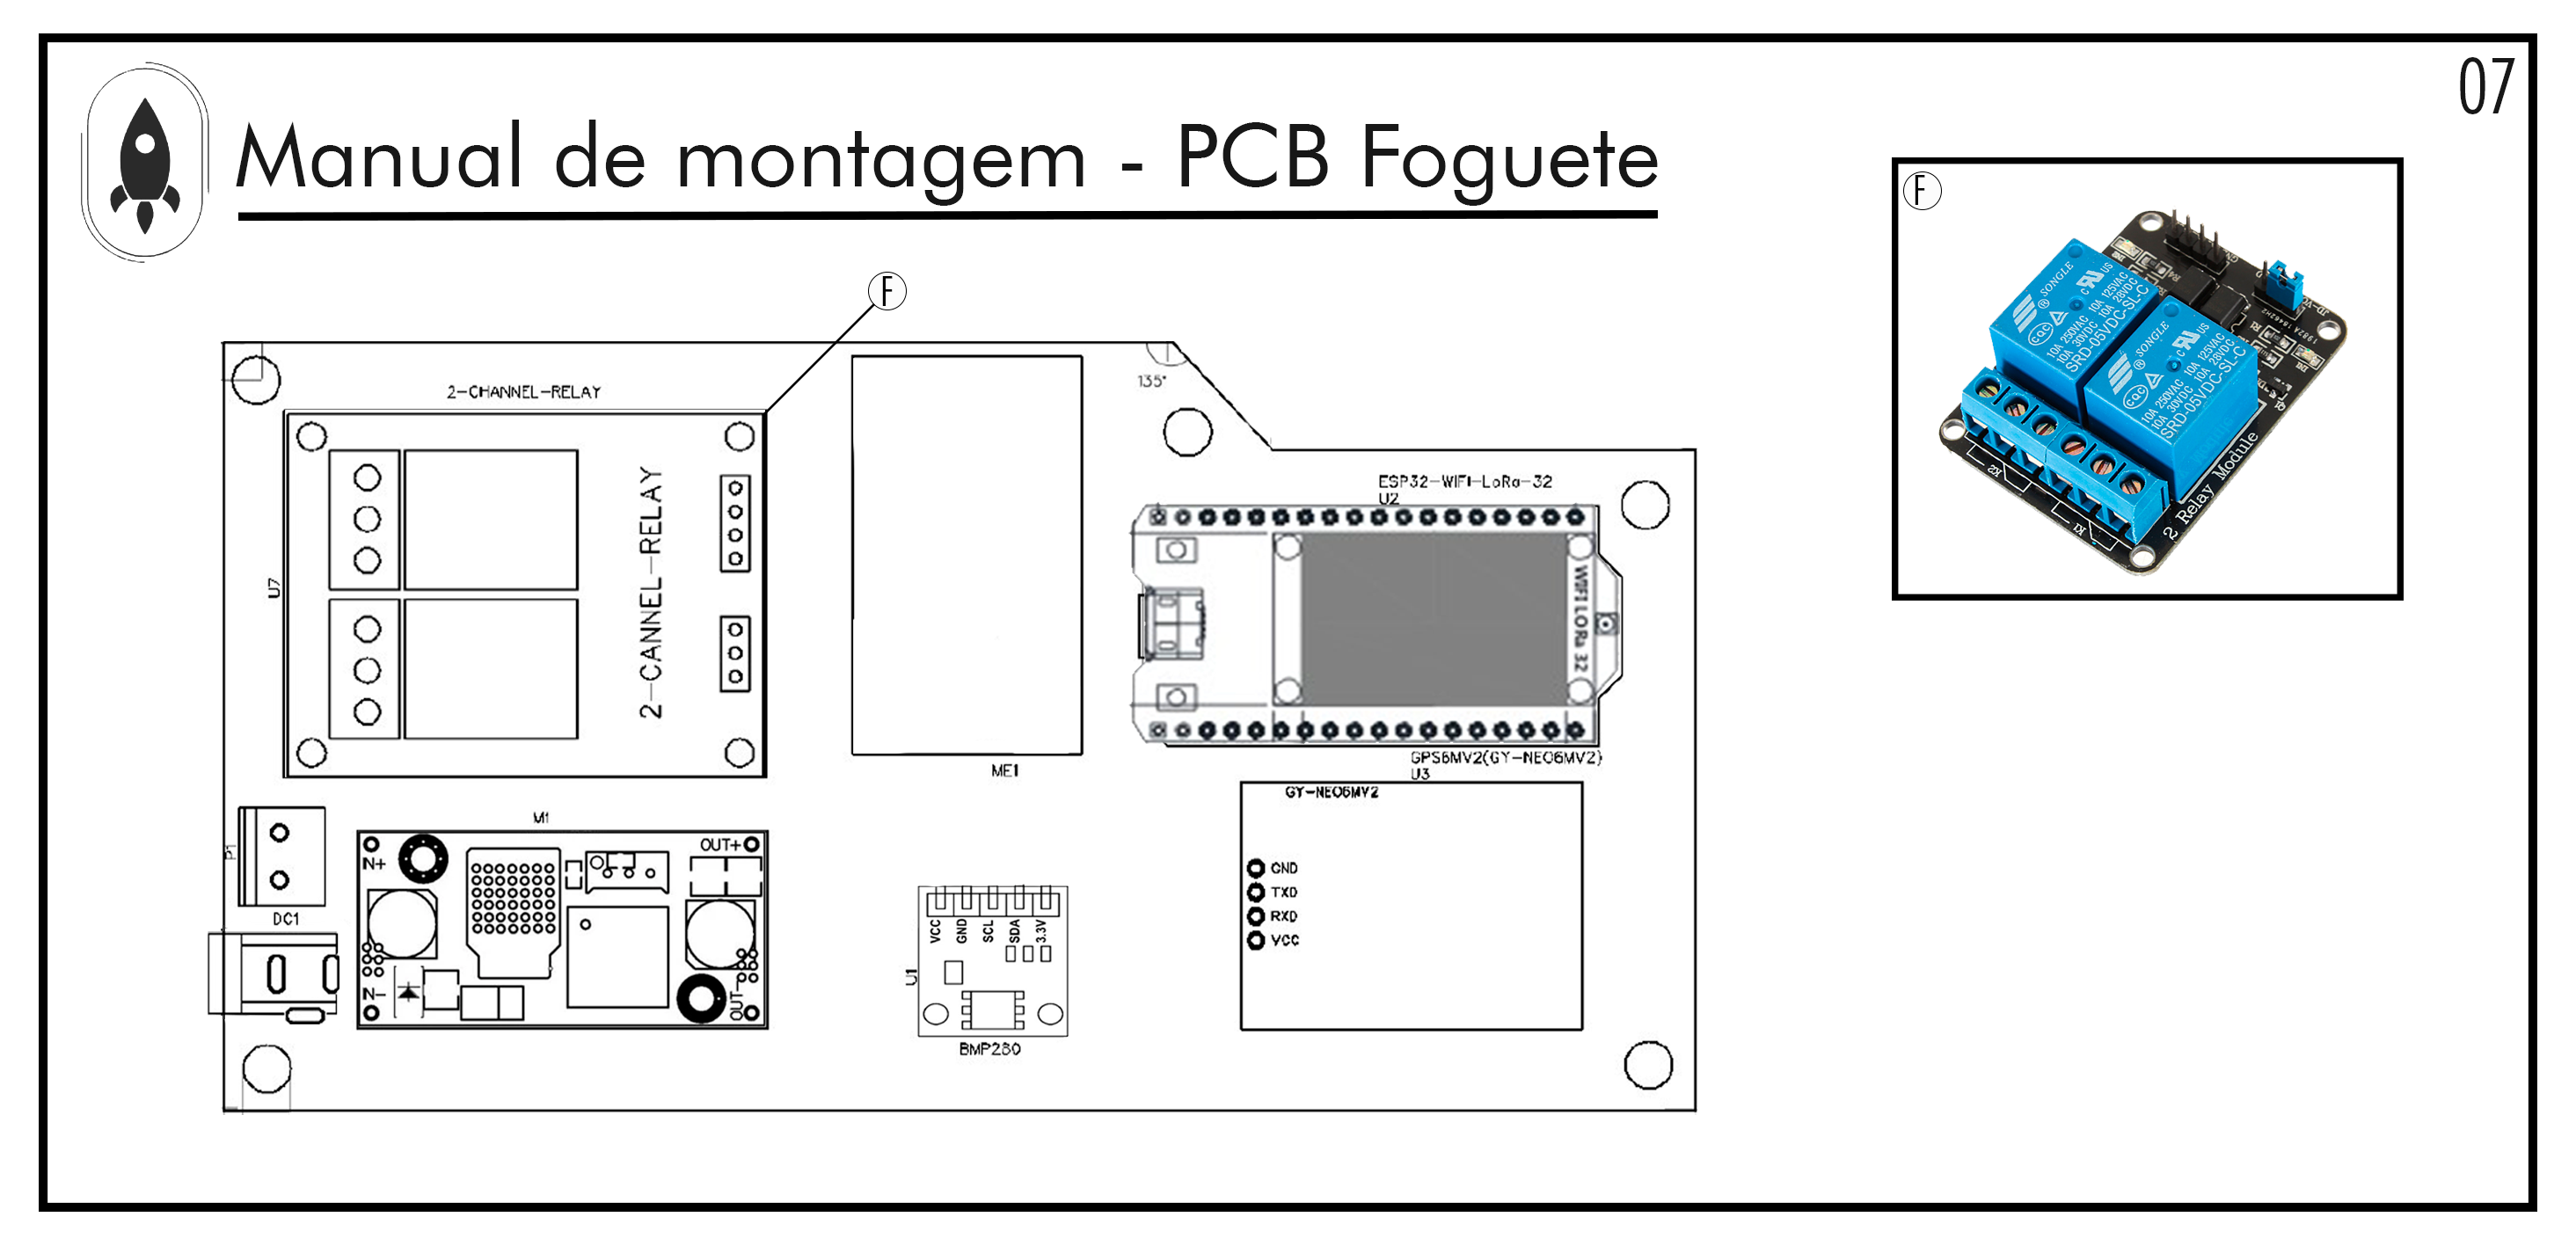
\includegraphics[width=\textwidth]{Figuras/FOGUETE/Pg-07---PL-02.png}
  \caption{Módulo Relé 5V 2 Canais modelo SRD-05VDC-SL-C.}
 %{ \footnotesize Fonte: Autores} 
  \label{fig:PCIFoguete Relé}
\end{figure}

\newpage

\par Pegue o componente 'G'(Módulo GPS GY-NEO6MV2), encaixe-a na posição mostrada \ref{fig:PCIBASE LORA} e solde junto a placa.
\begin{figure}[H]
  \centering
  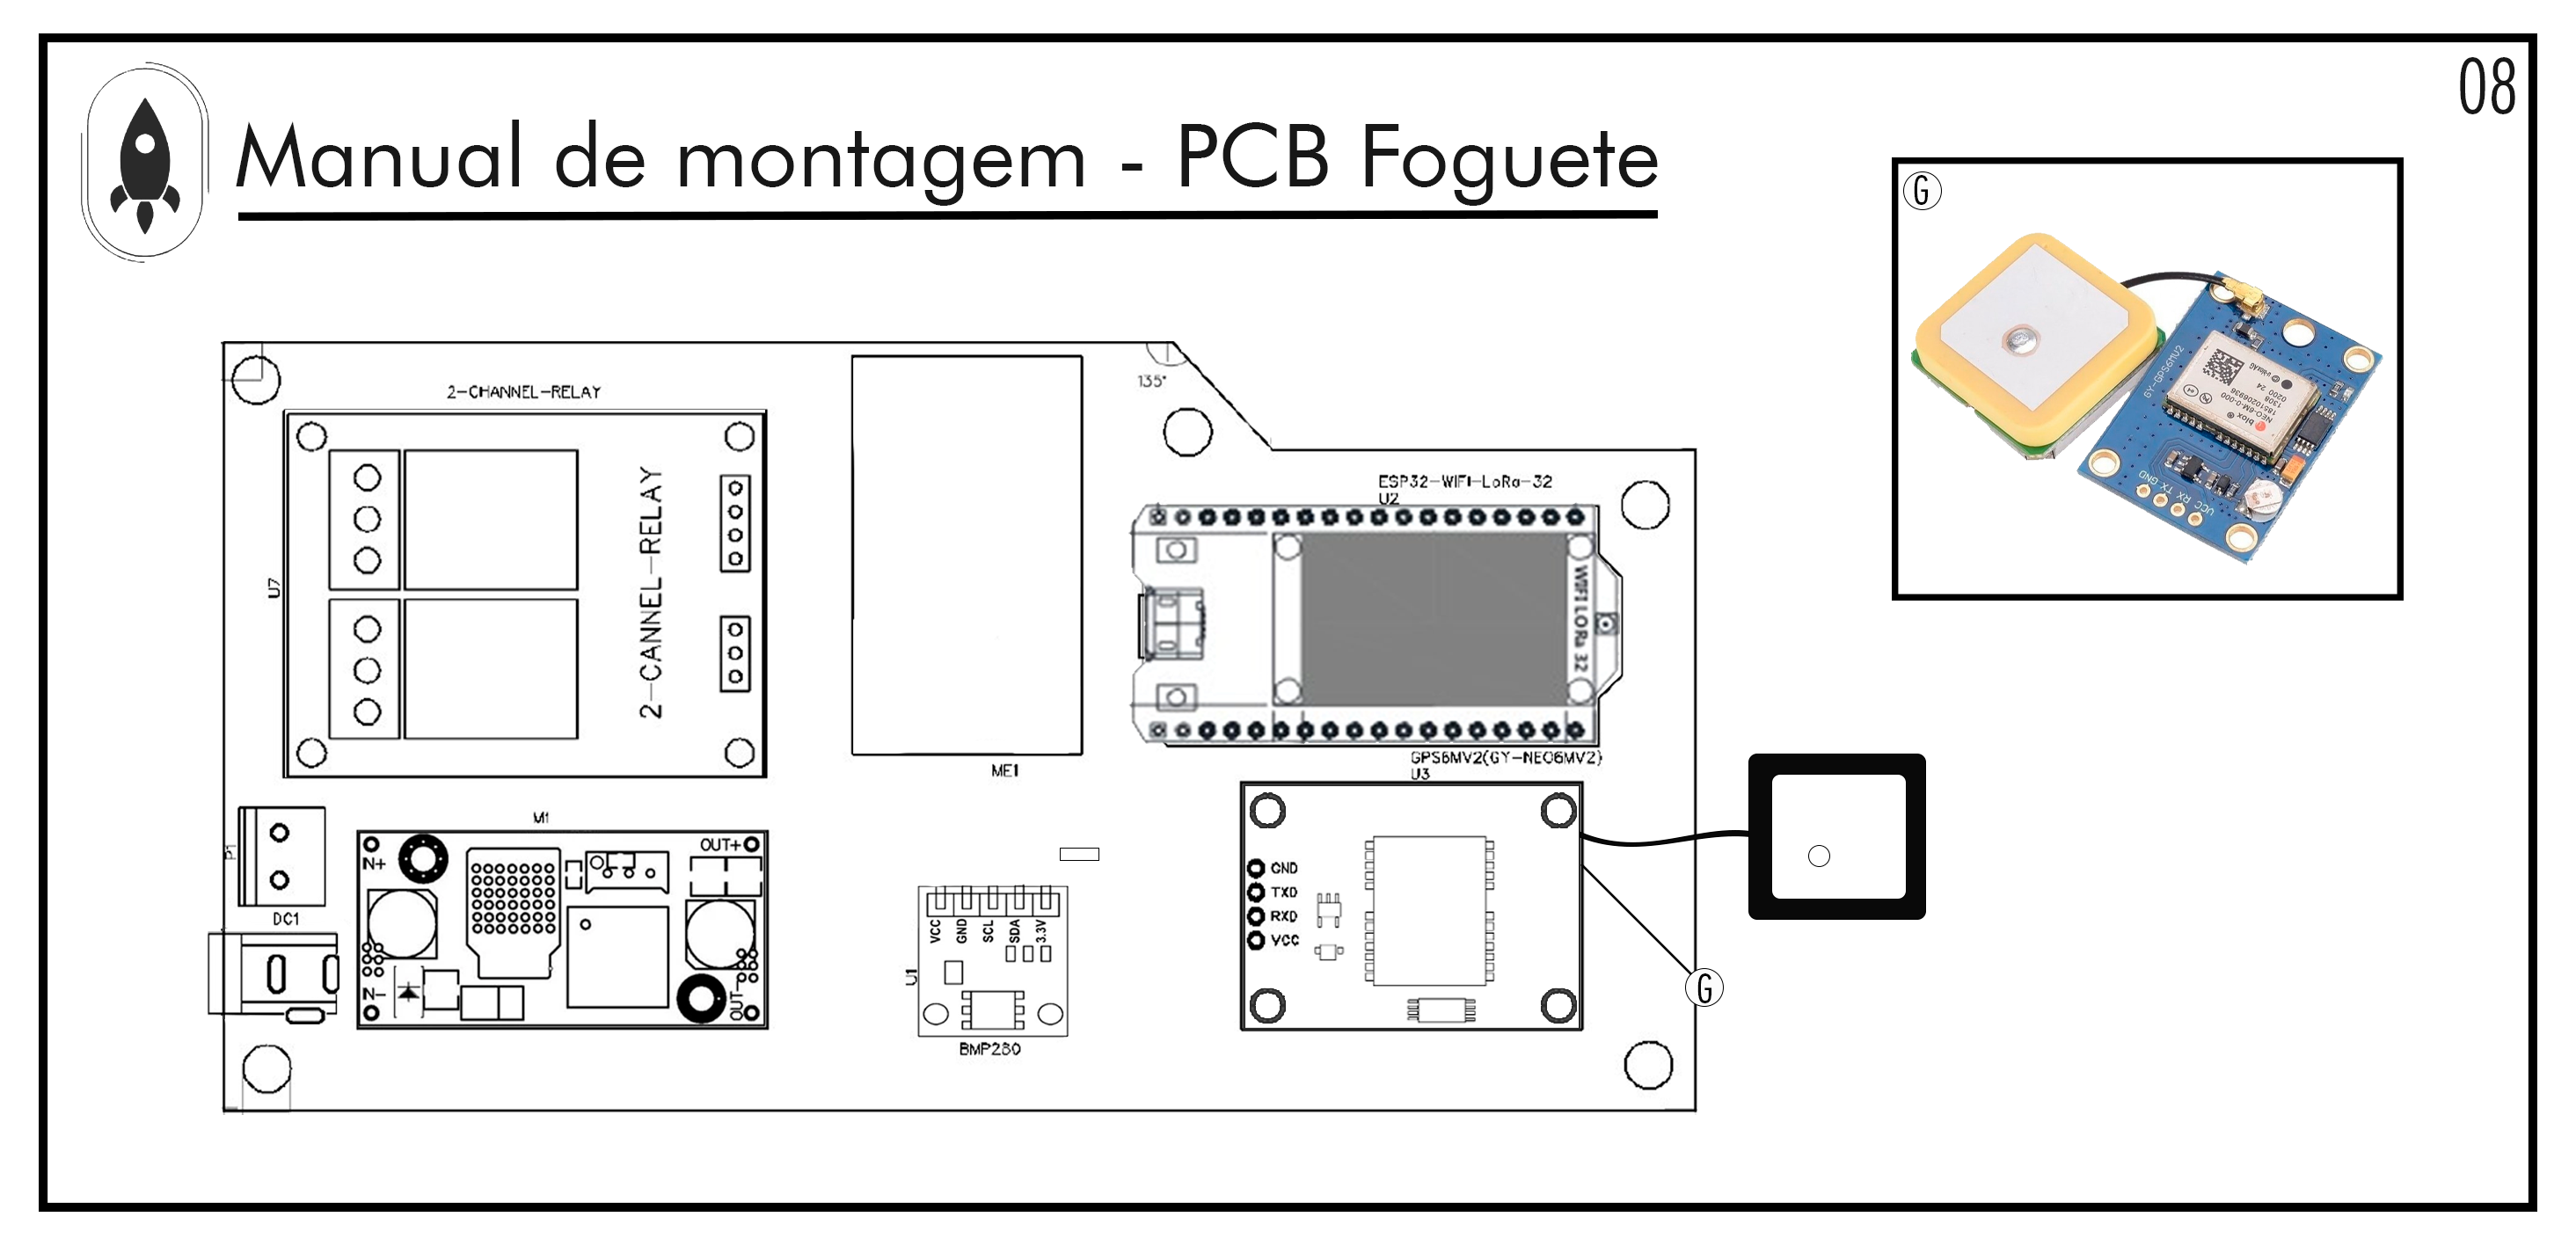
\includegraphics[width=\textwidth]{Figuras/FOGUETE/Pg-08---PL-02.png}
  \caption{Módulo GPS GY-NEO6MV2.}
 %{ \footnotesize Fonte: Autores} 
  \label{fig:PCIFoguete LORA}
\end{figure}


\par Pegue o componente 'H'(Módulo Cartão de Memoria), encaixe-a na posição mostrada \ref{fig:PCIFoguete MICRO SD CARD} e solde junto a placa.
\begin{figure}[H]
  \centering
  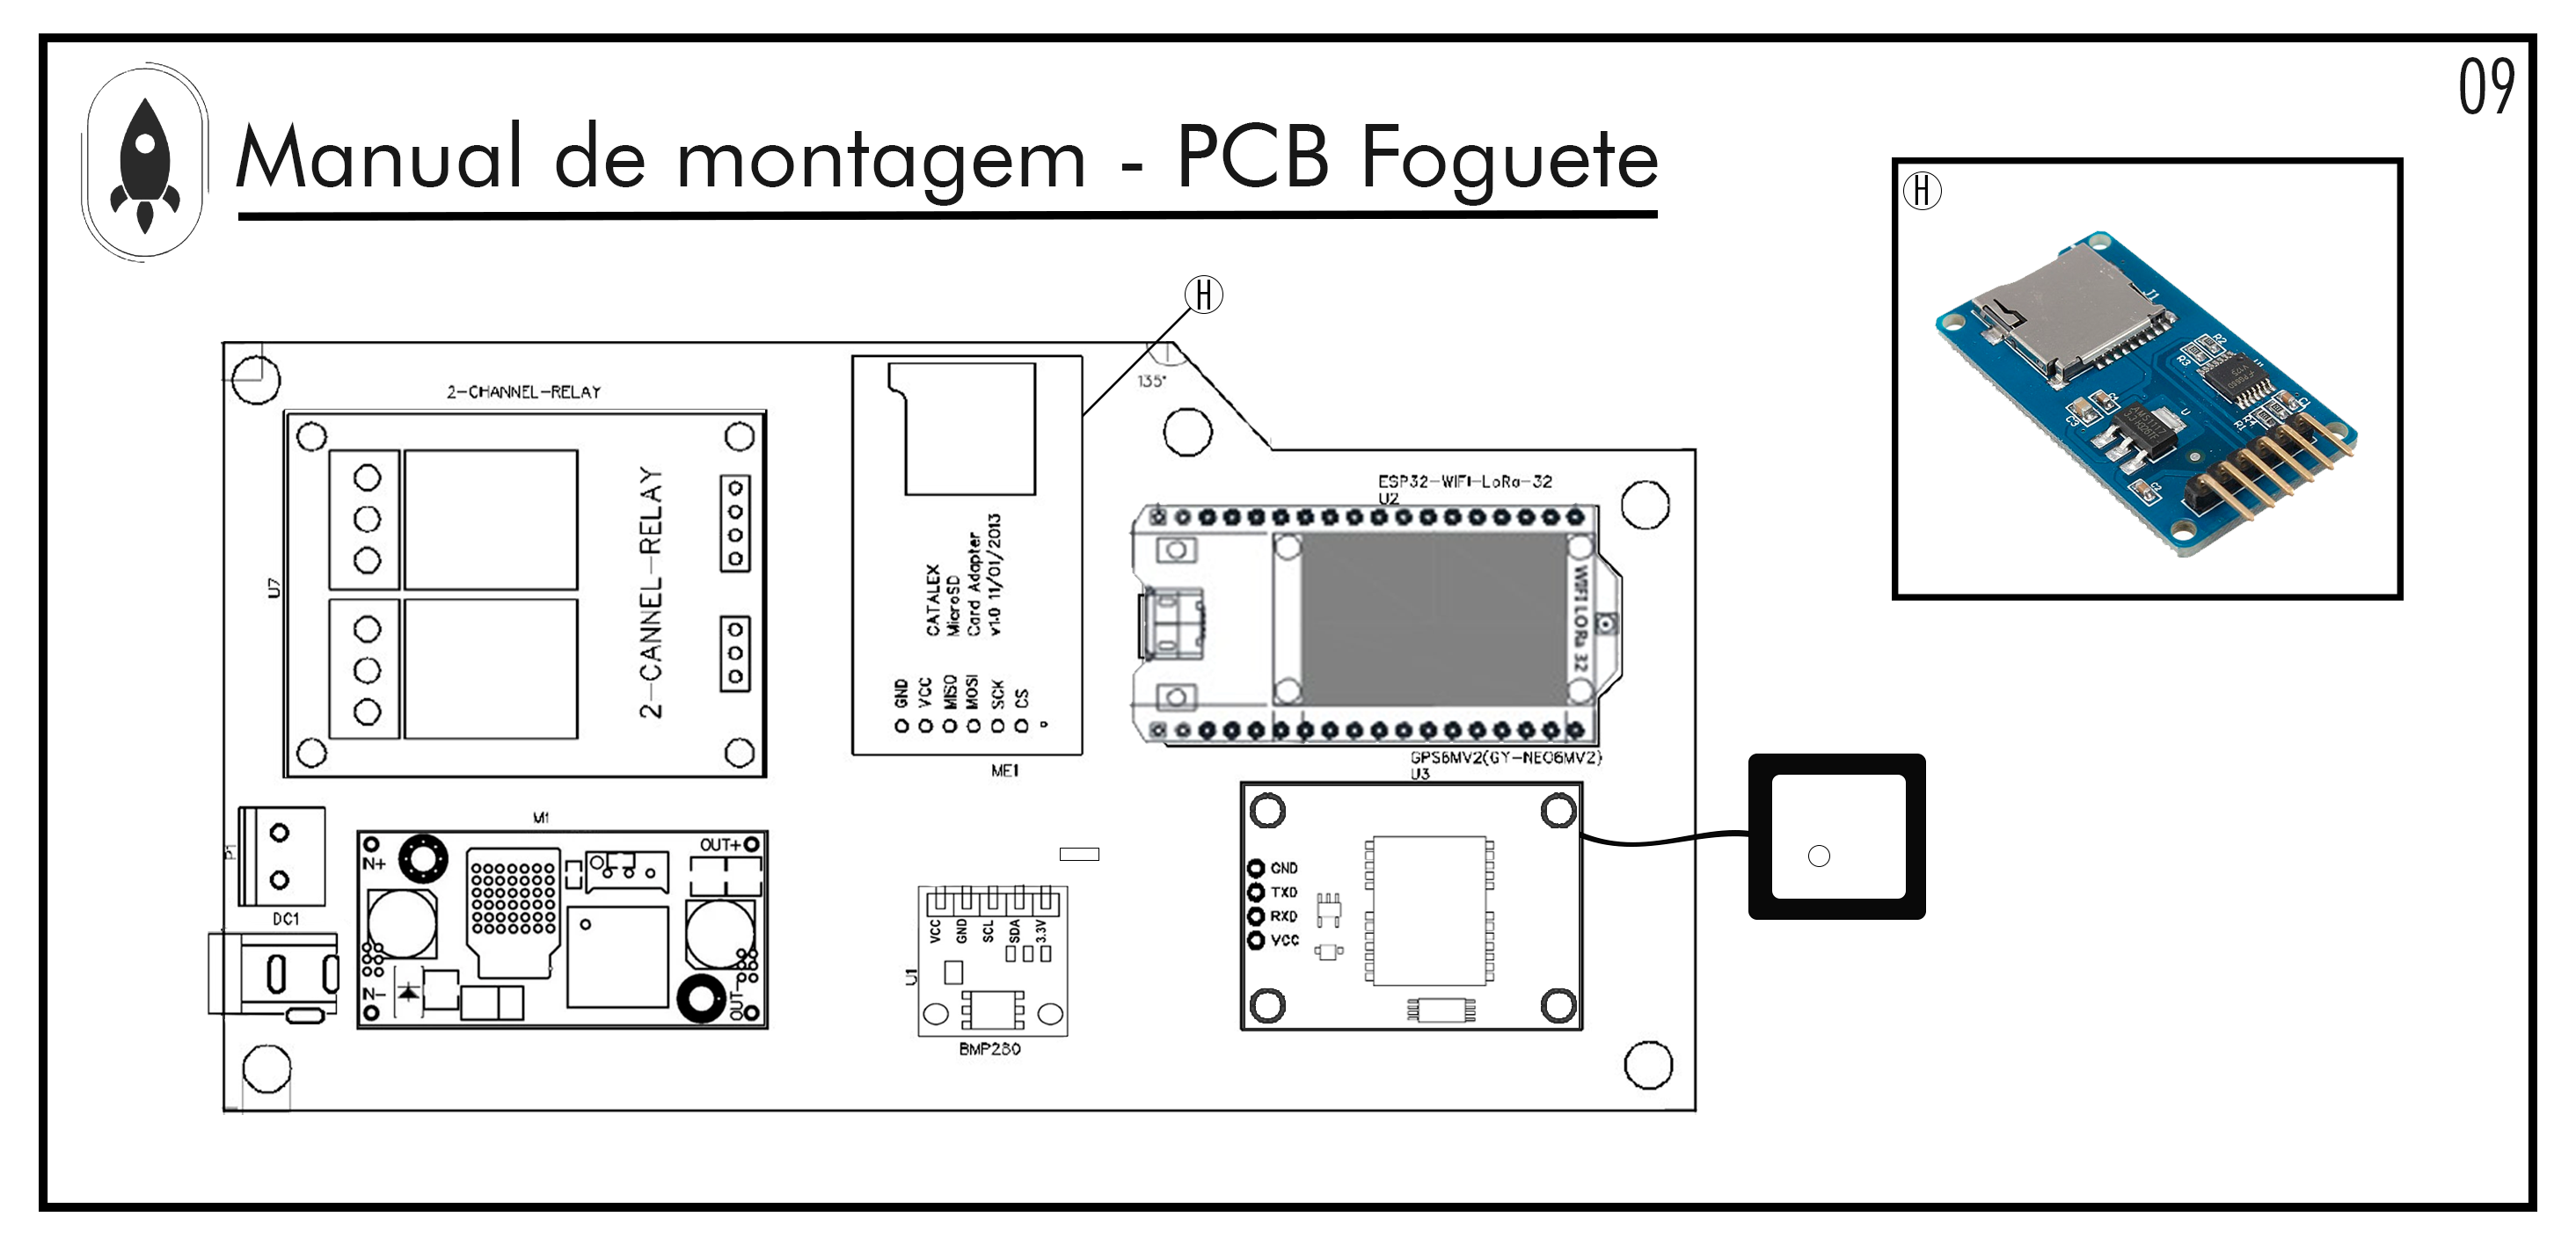
\includegraphics[width=\textwidth]{Figuras/FOGUETE/Pg-09---PL-02.png}
  \caption{Módulo Cartão de Memoria.}
 %{ \footnotesize Fonte: Autores} 
  \label{fig:PCIFoguete MICRO SD CARD}
\end{figure}

\newpage

\par Pegue o componente 'I'(Conector Borne KRE 2 Vias), encaixe-a na posição mostrada \ref{fig:PCIFoguete Borne} e solde junto a placa.
\begin{figure}[H]
  \centering
  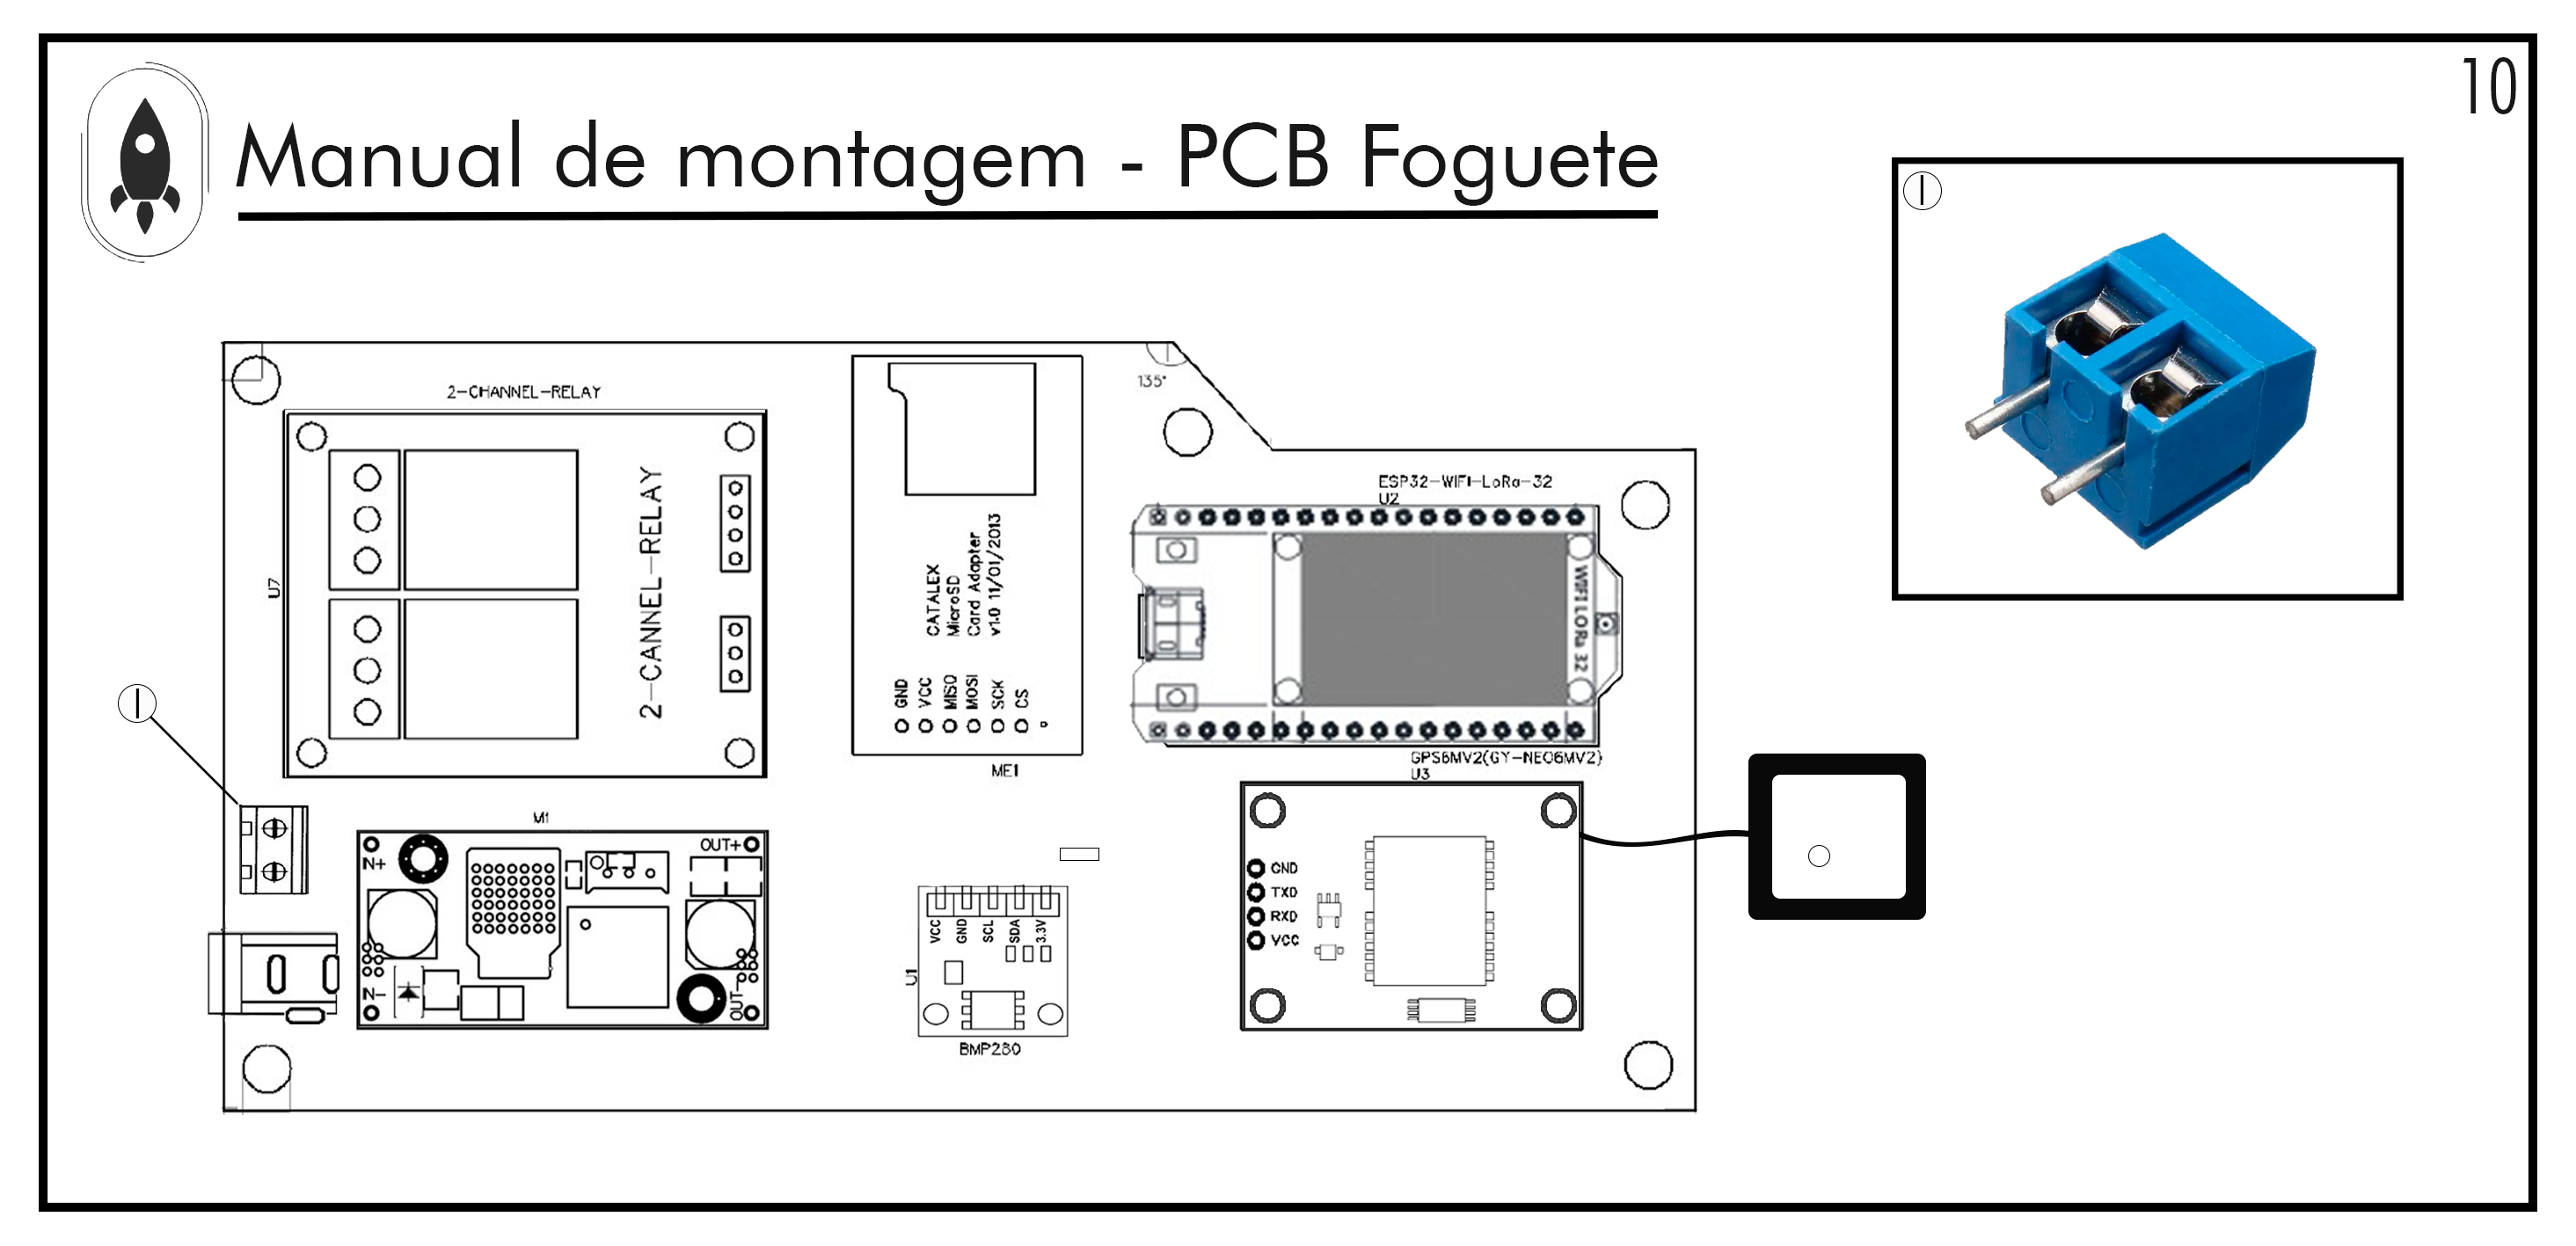
\includegraphics[width=\textwidth]{Figuras/FOGUETE/Pg-10---PL-02.png}
  \caption{Conector Borne KRE 2 Vias.}
 %{ \footnotesize Fonte: Autores} 
  \label{fig:PCIFoguete Borne}
\end{figure}
\par Para a fixação da placa em seu recipiente utilize os parafusos e a porca extensora, componentes 'J' e 'K' e siga as instruções da seção \ref{sec:fixação }.

\newpage

\subsection{Placas de Circuito Impresso-Maleta Interface do usuário}

\par Primeiramente é necessário ter em mão todos os componentes para sua montagem \ref{fig:Lista de materiasi MALETA}.

\subsubsection{Lista de Materiais}

\par Primeiramente é necessário ter em mão todos os componentes para sua montagem \ref{fig:Lista de materiais MALETA1}.

\begin{table}[H]
\centering
\begin{tabular}{|m{1.9cm} |m{1.8cm} |m{7.3cm}|m{4cm}|}
\hline
\begin{center}Identificador\end{center} &\begin{center} Quantidade\end{center} & \begin{center}Componente\end{center} &\begin{center} Part Number\end{center} \\\hline
A&01 &  PCI- Maleta  & -  \\\hline

B&02 & Conector Adaptador Plug P4 Macho com Borne &  P4 Macho F0503 \\\hline
C&01 & Micro Usb V8 Macho & J5415\\\hline
D&01 & Plug Hdmi Macho & Hdmi Macho \\\hline
E&01 & Conector Jack J4 DC Fêmea &  Jack Fêmea  \\\hline
F&01 & Chave Gangorra 2 Polos Mini  & Kcd11-101   \\\hline
G &01&Lora Esp32 Sx1278 Com Display  Oled Wifi bluetooth 915mhz& Sx1278 \\\hline
H & 01 & NVIDIA Jetson Nano Developer Kit  & 945-13450-0000-100\\\hline 
I & 01 &Placa controladora   & PCB800099-V.9  \\\hline 
J& 01 &  Conversor DC-DC Step Down-LM2596 (12~5V)
& LM2596 \\\hline
K &01& Display LCD 9 polegadas  & Lcd 9" TMOEC \\\hline
L& 01&Mini  Teclado  slim  com  Touchpad & -  \\\hline
\end{tabular}
\caption{Lista de componentes}
\end{table}


\subsubsection{Instruções}

\begin{figure}[H]
  \centering
  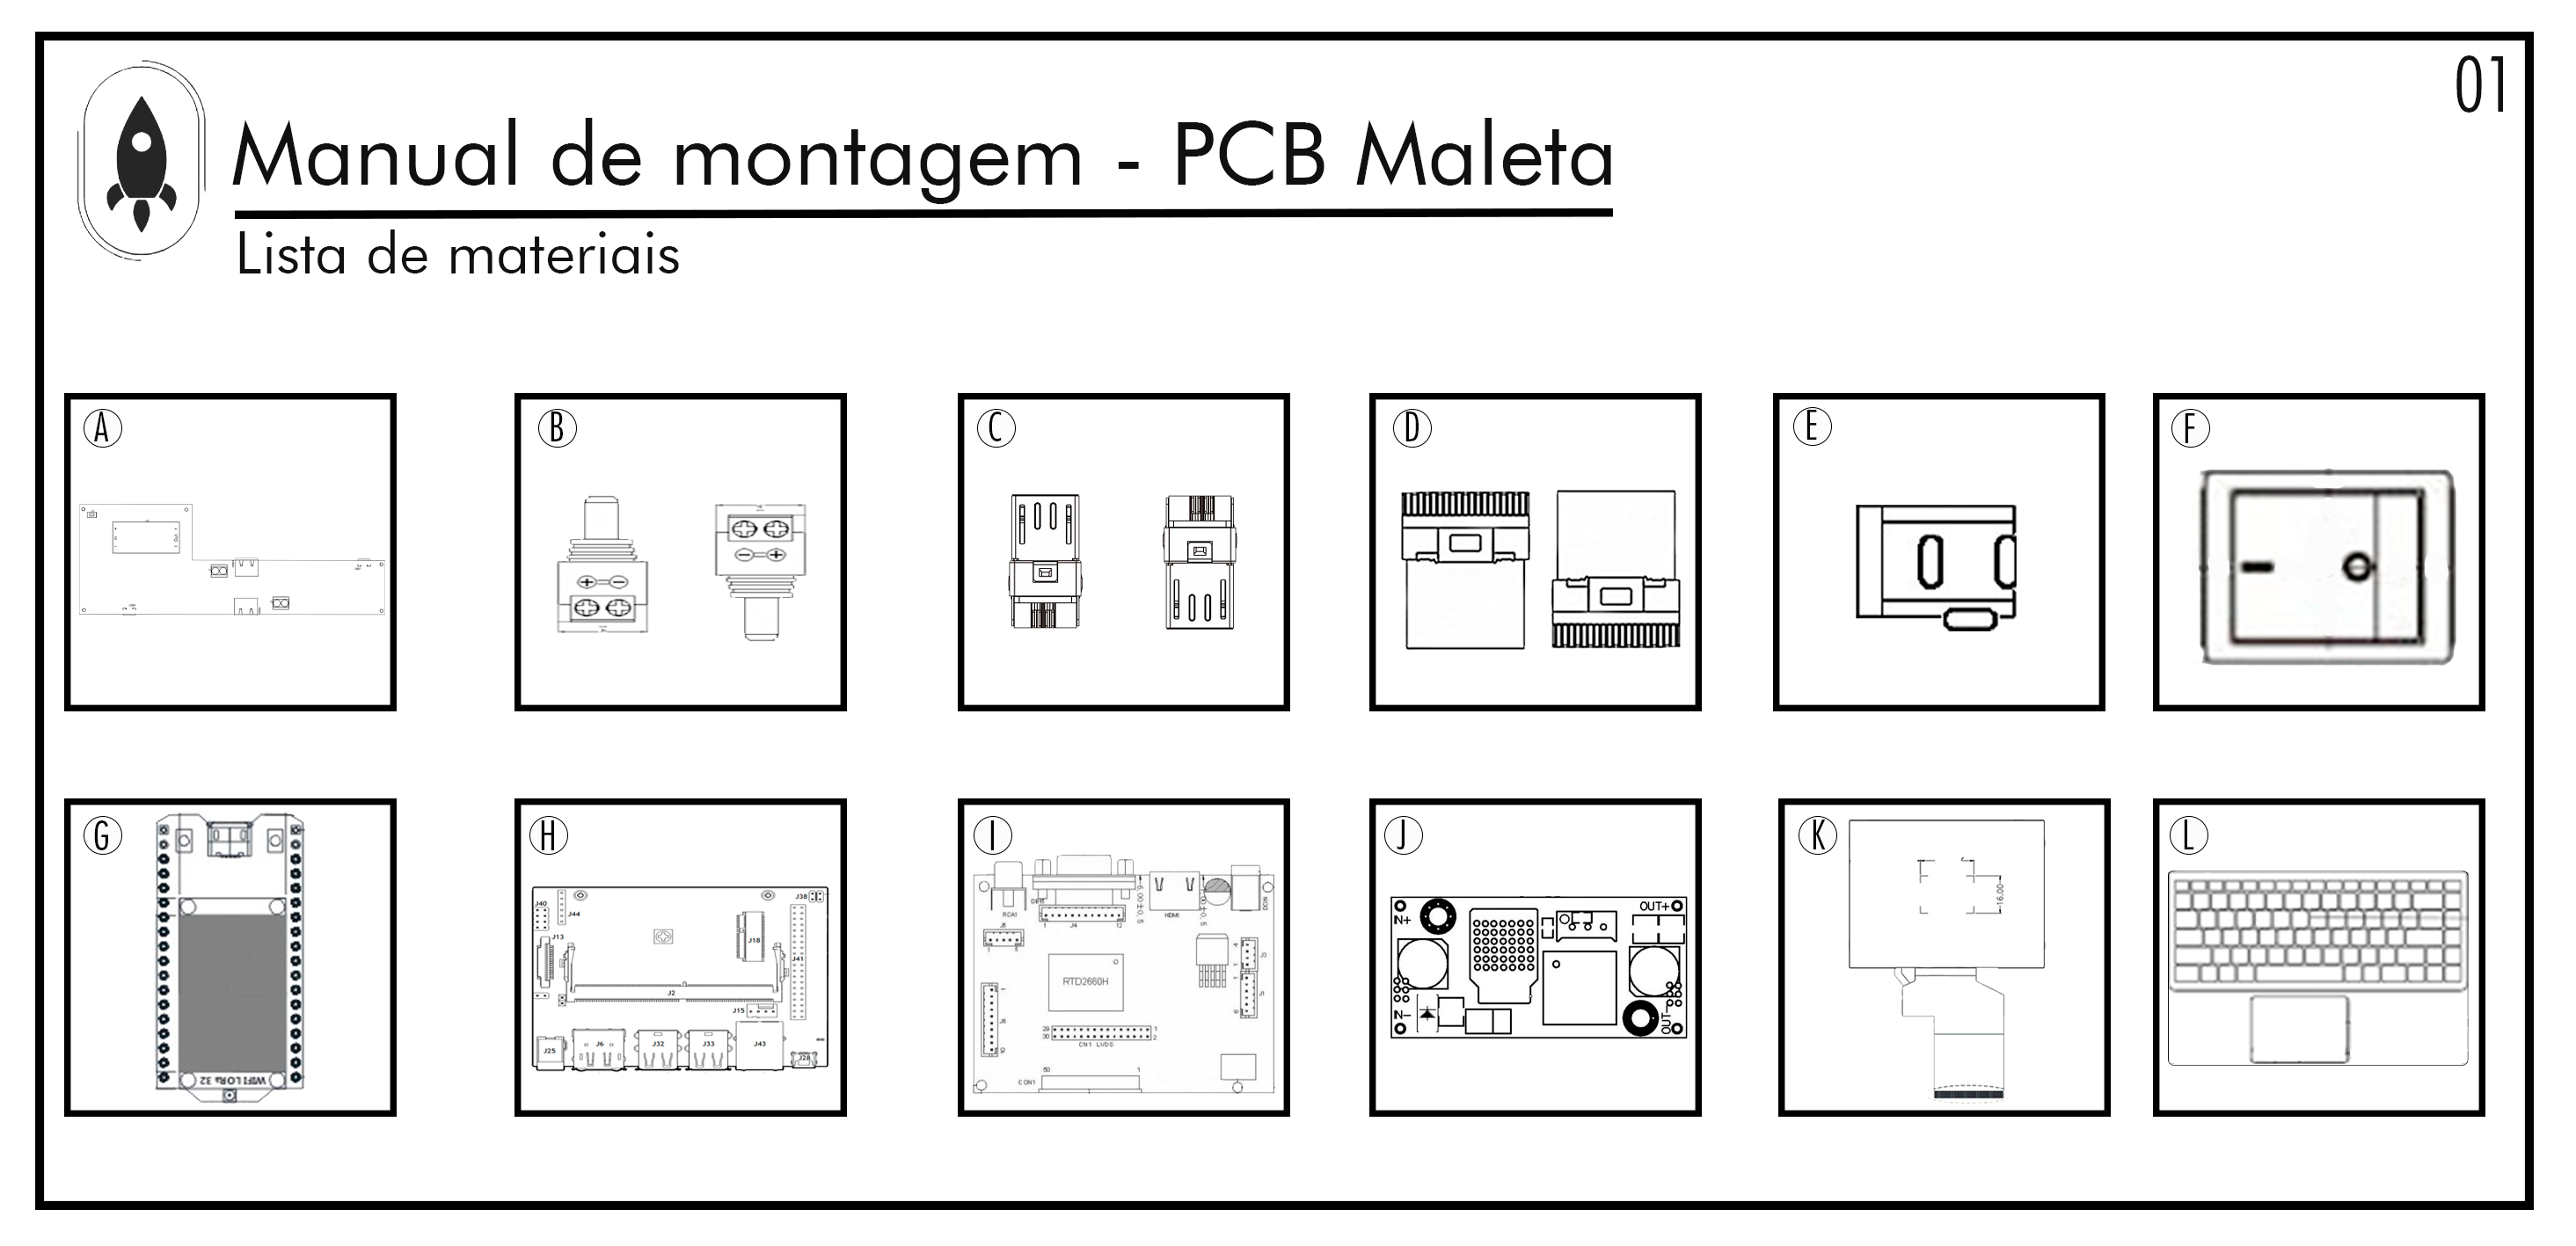
\includegraphics[width=\textwidth]{Figuras/MALETA/Pg-01---PL-01.png}
  \caption{Lista de Materiais.} 
 %{ \footnotesize Fonte: Autores} 
  \label{fig:Lista de materiais MALETA1}
\end{figure}


 \par Com todos os componentes em mãos, pegue componente 'A'(PCI-MALETA) prepare-a para soldagem dos componentes passando uma fina camada de solda nos pads da PCI.

\begin{figure}[H]
  \centering
  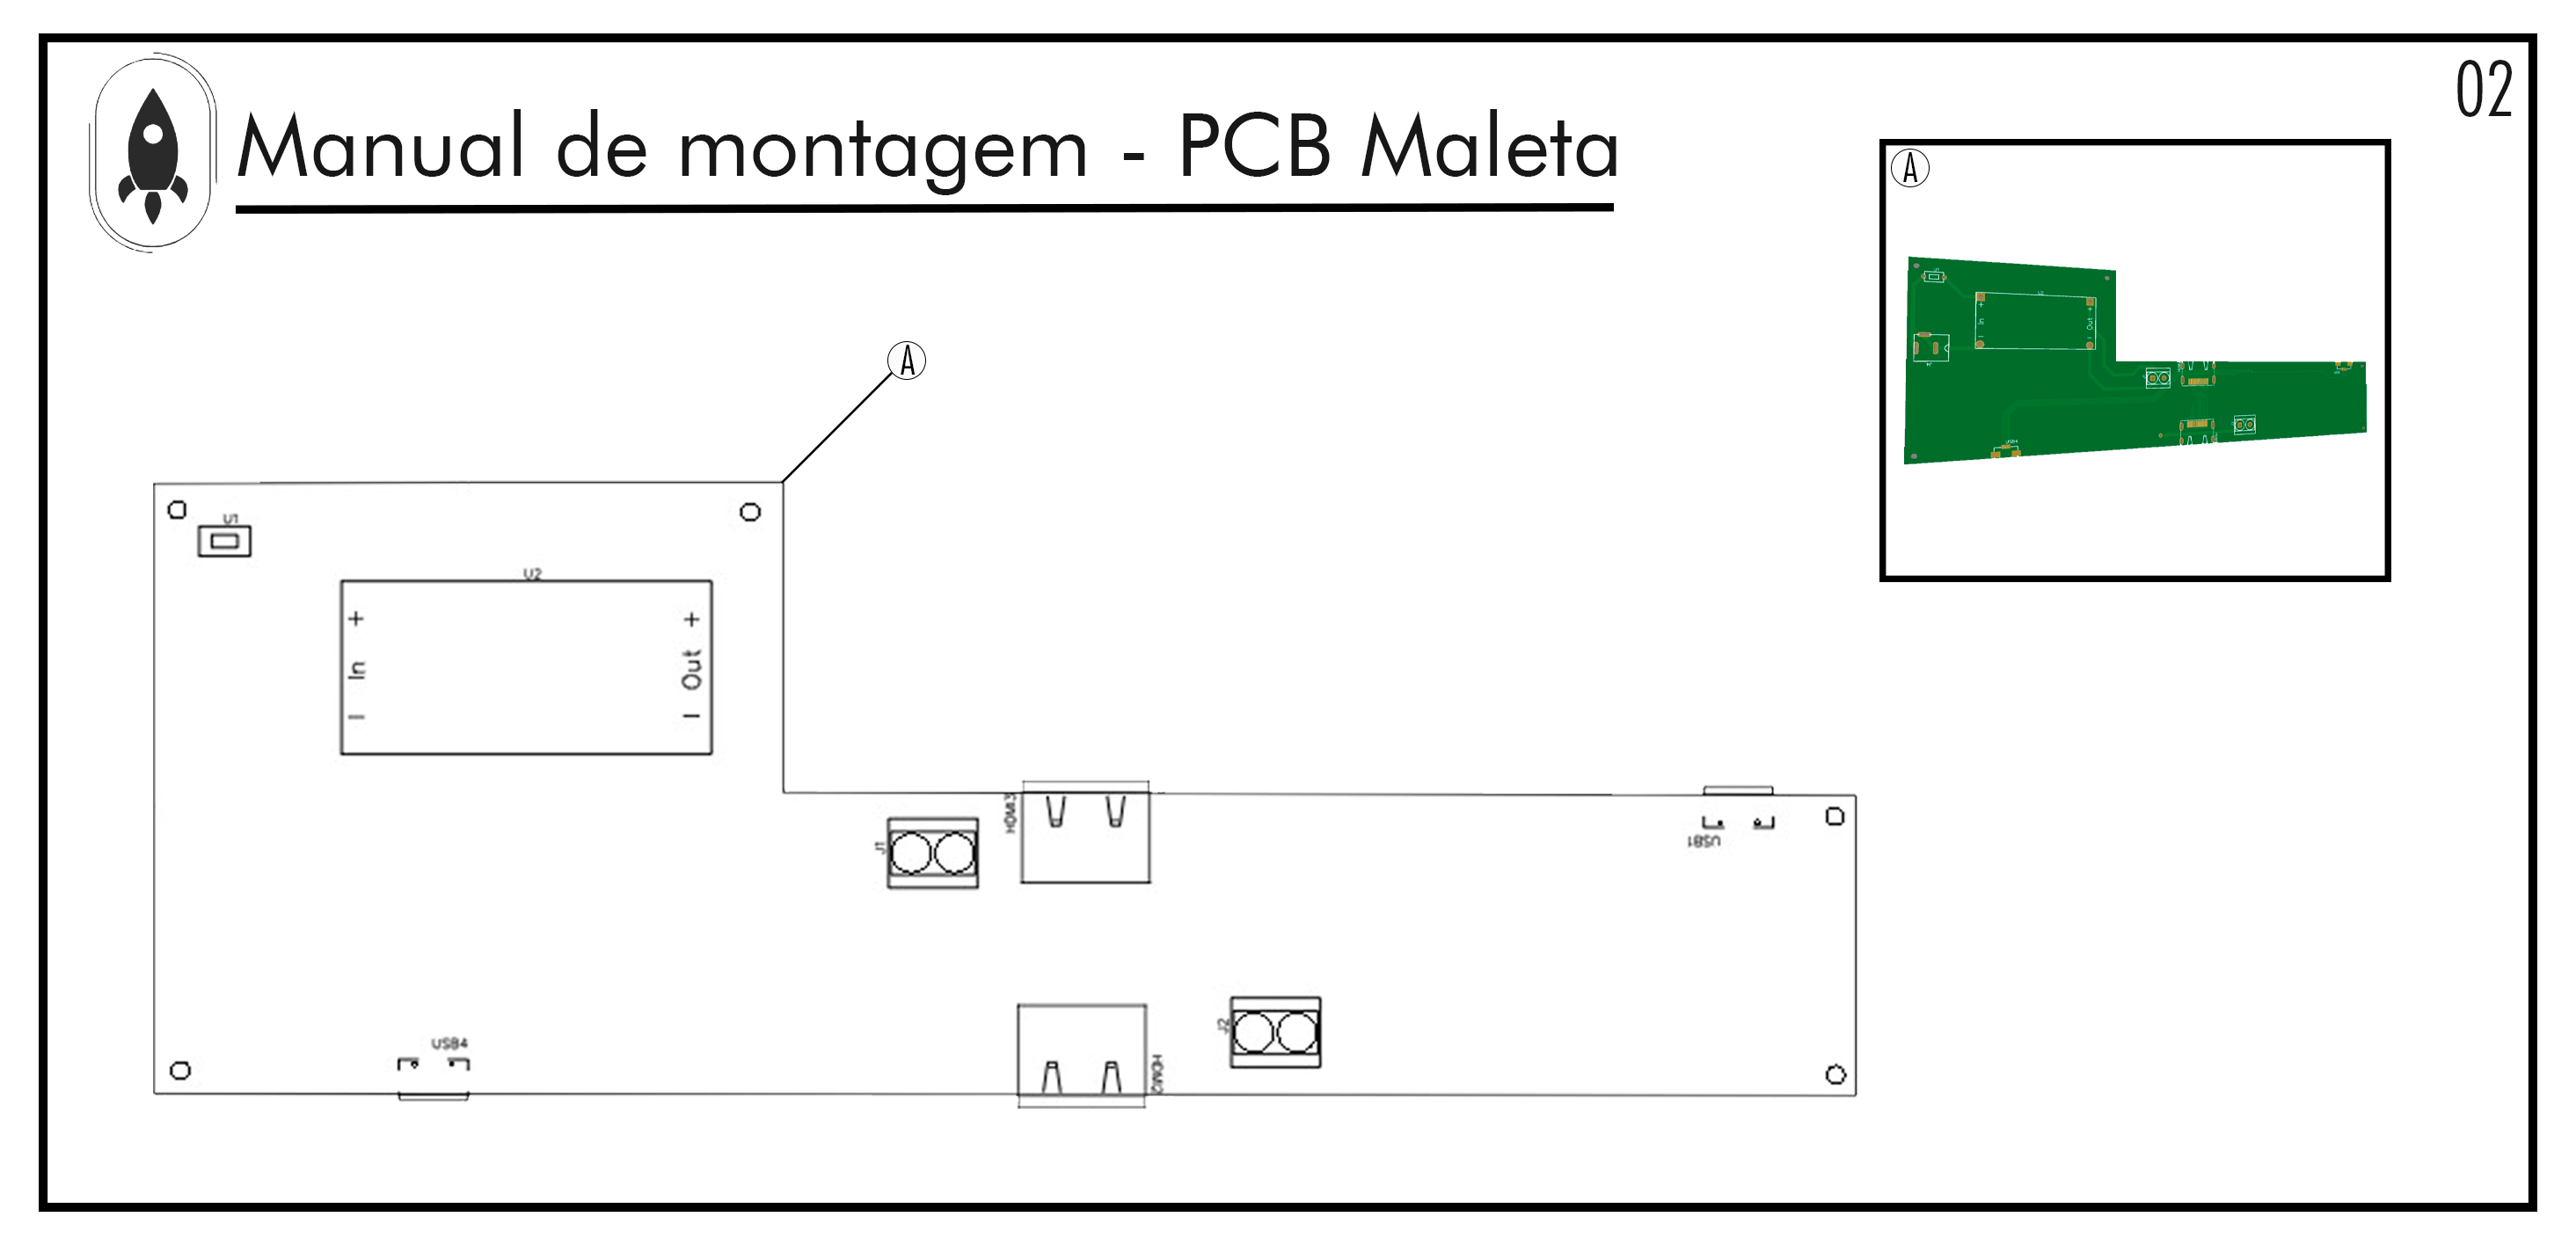
\includegraphics[width=\textwidth]{Figuras/MALETA/Pg-02---PL-01.png}
  \caption{PCI da maleta do usuário.}
 %{ \footnotesize Fonte: Autores} 
  \label{fig:Lista de materiasi MALETA}
\end{figure}
\newpage

\par Pegue o componente 'B'Conector Adaptador Plug P4 Macho com Borne ), encaixe-a na posição mostrada \ref{fig:PCBMALETA Jack} e solde junto a placa.
\begin{figure}[H]
  \centering
  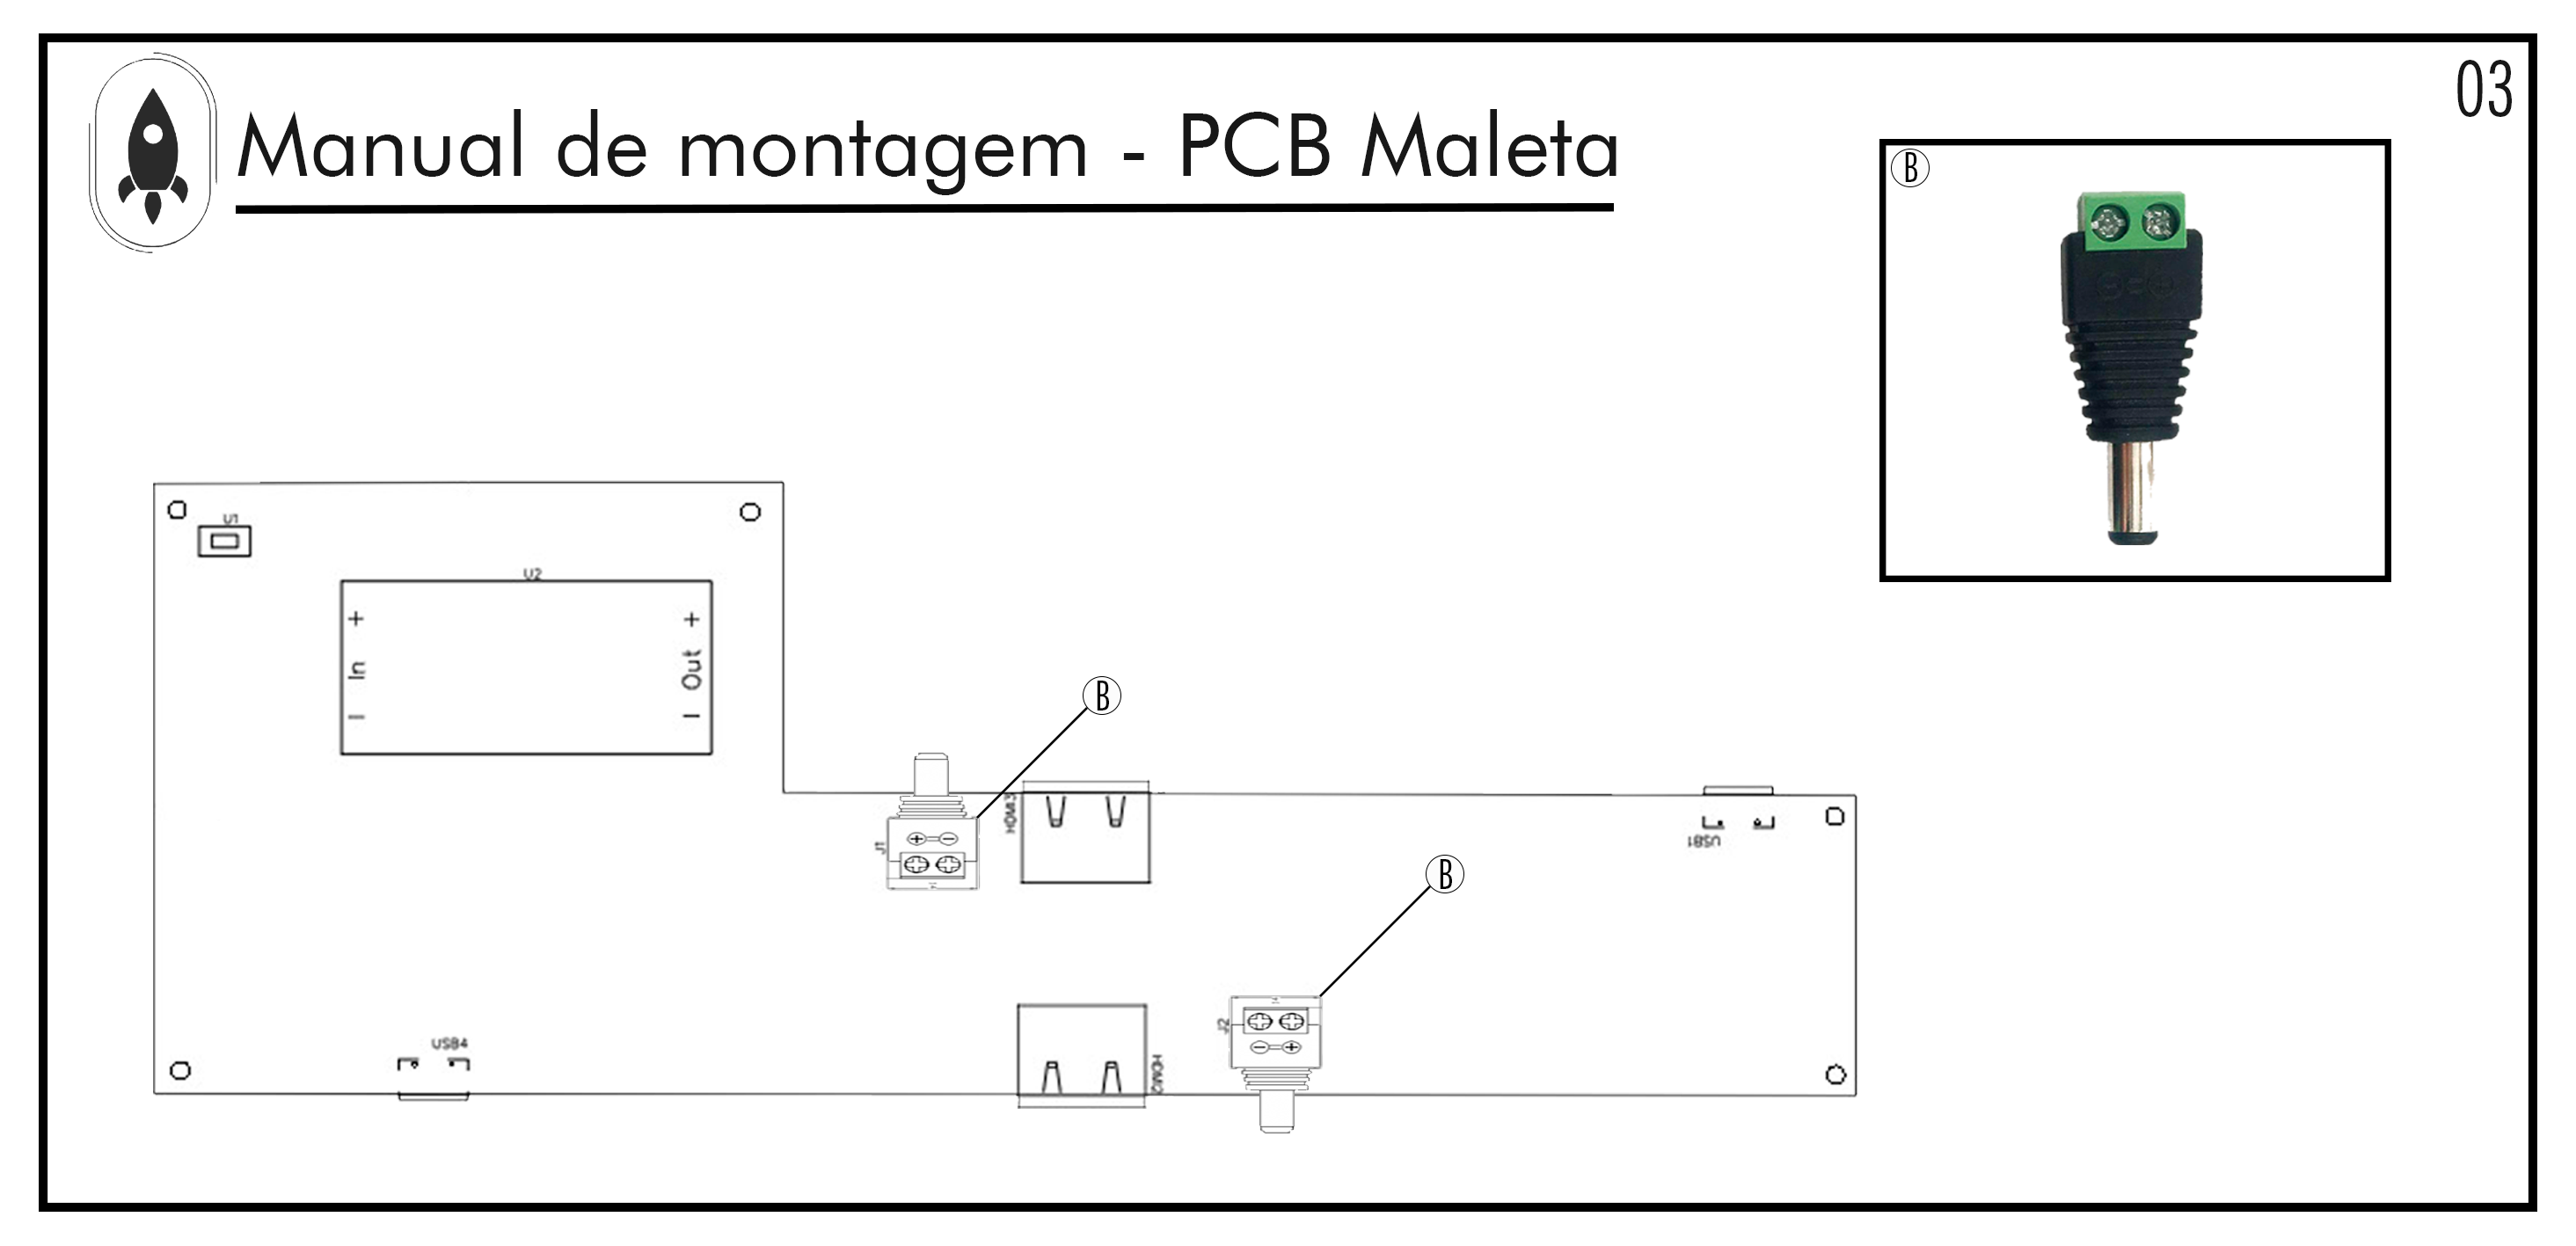
\includegraphics[width=\textwidth]{Figuras/MALETA/Pg-03---PL-01.png}
  \caption{Adaptador Jack DC macho.}
 %{ \footnotesize Fonte: Autores} 
  \label{fig:PCBMALETA Jack}
\end{figure}


\par Pegue o componente 'C'(Micro Usb V8 Macho), encaixe-a na posição mostrada \ref{fig:PCBMALETA Micro Usb} e solde junto a placa.

\begin{figure}[H]
  \centering
  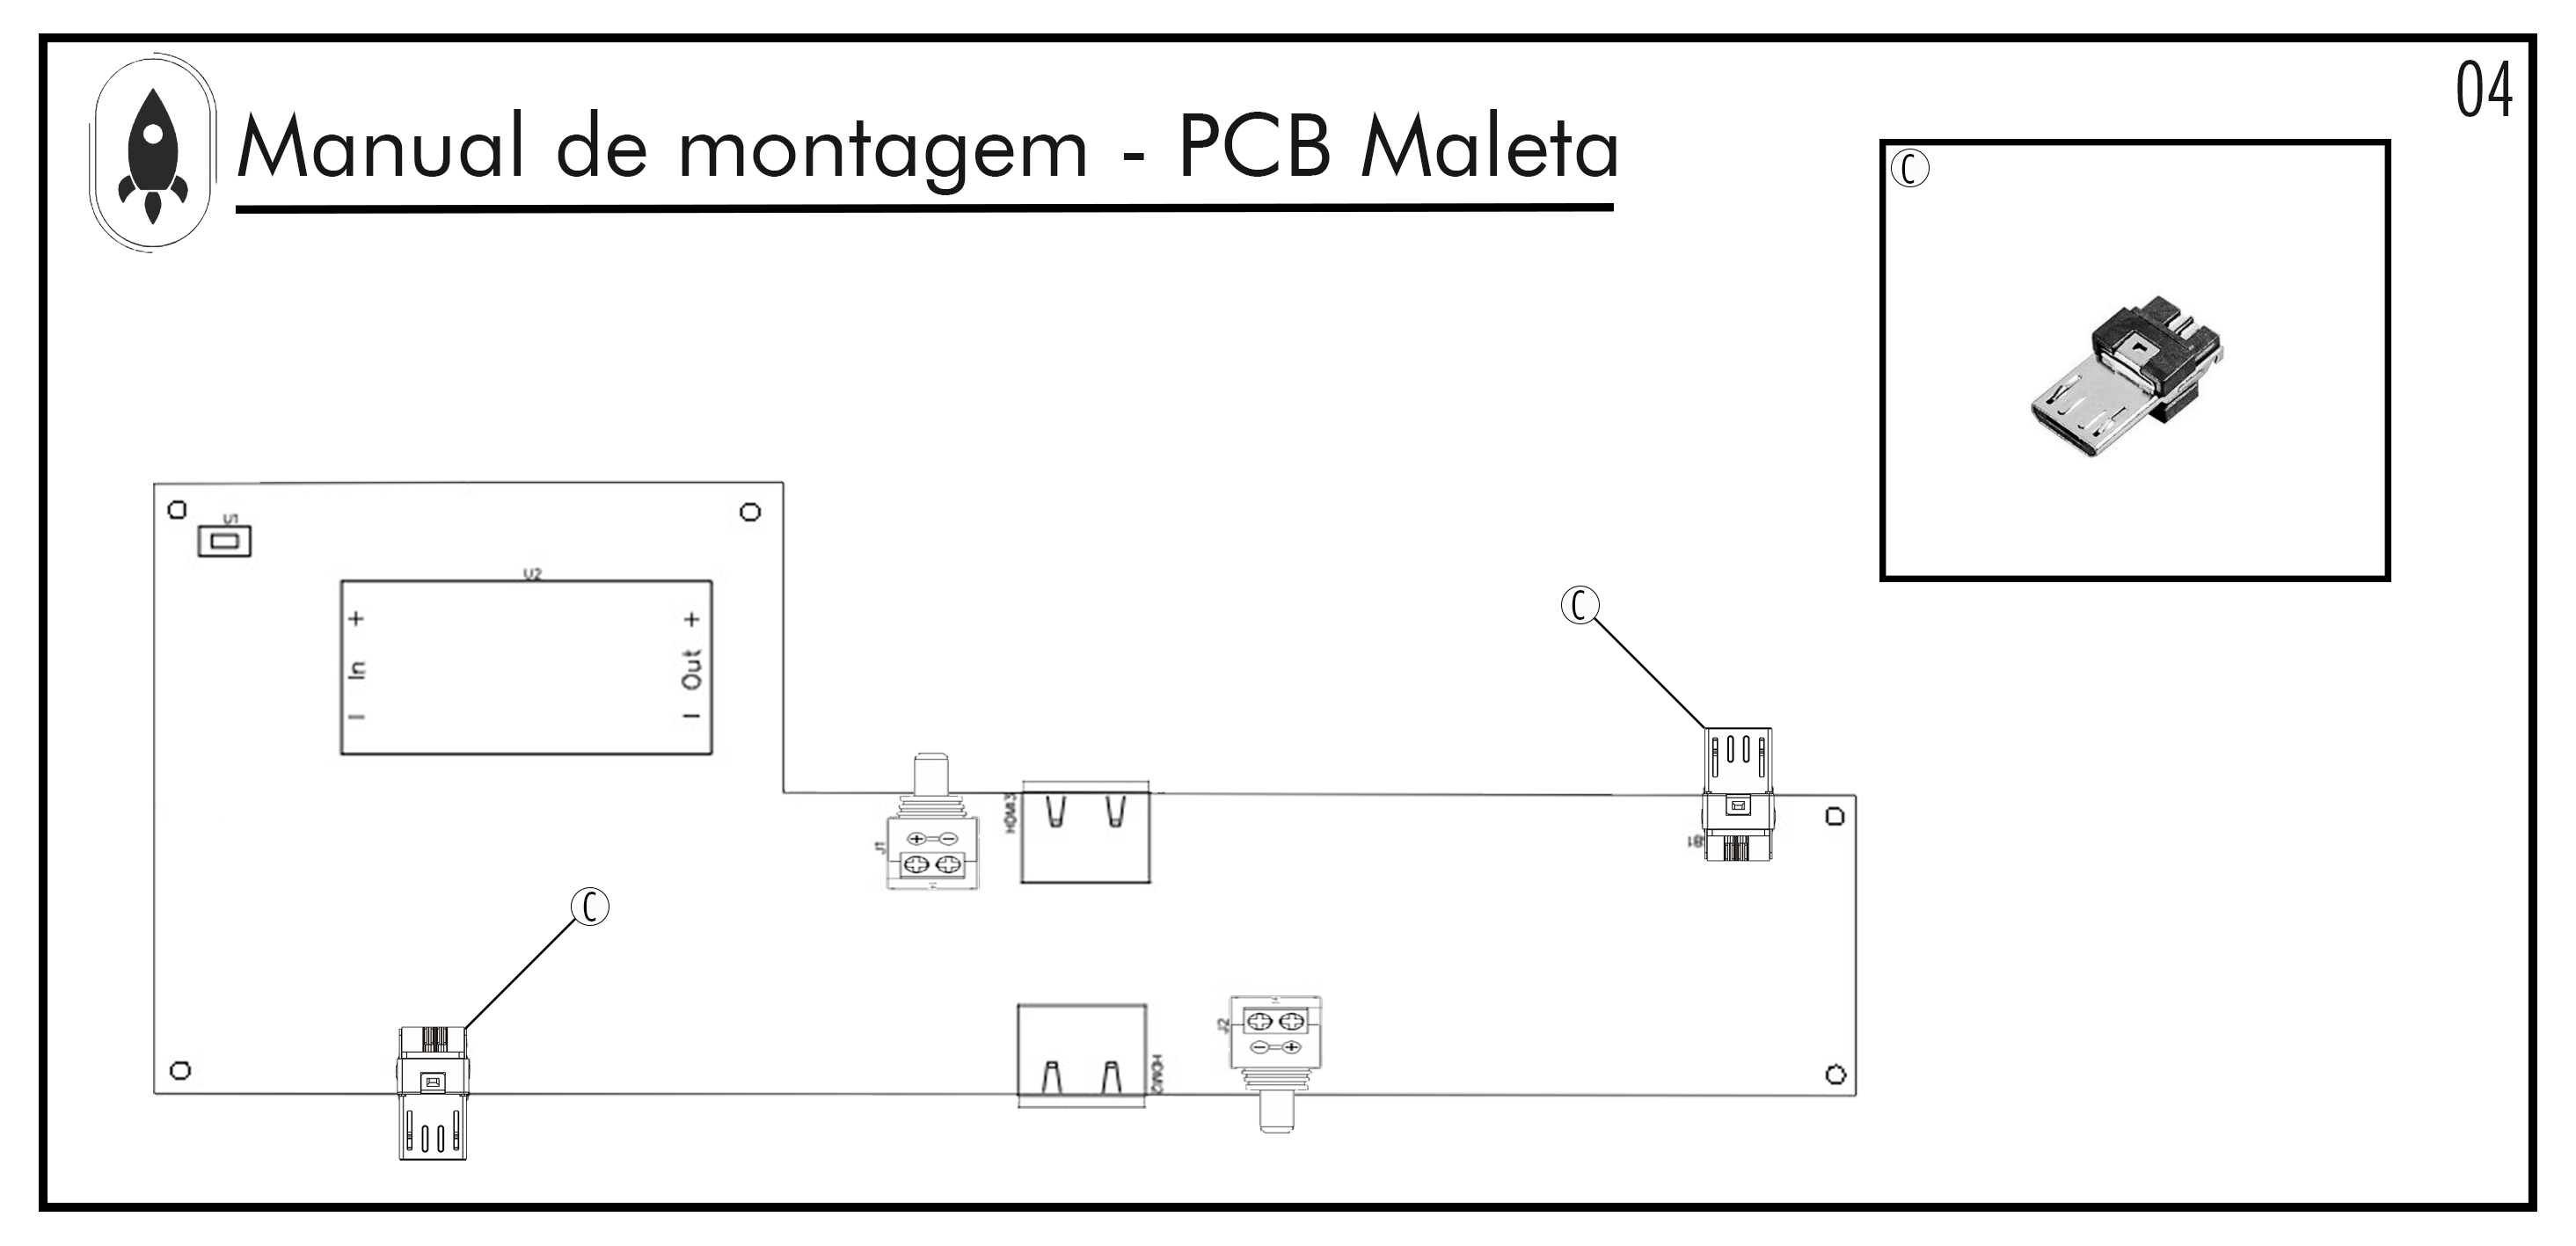
\includegraphics[width=\textwidth]{Figuras/MALETA/Pg-04---PL-01.png}
  \caption{Micro Usb V8 Macho.}
 %{ \footnotesize Fonte: Autores} 
  \label{fig:PCBMALETA Micro Usb}
\end{figure}

\newpage

\par Pegue o componente 'D'(Plug Hdmi Macho), encaixe-a na posição mostrada \ref{fig:PCBMALETA Hdmi} e solde junto a placa.
\begin{figure}[H]
  \centering
  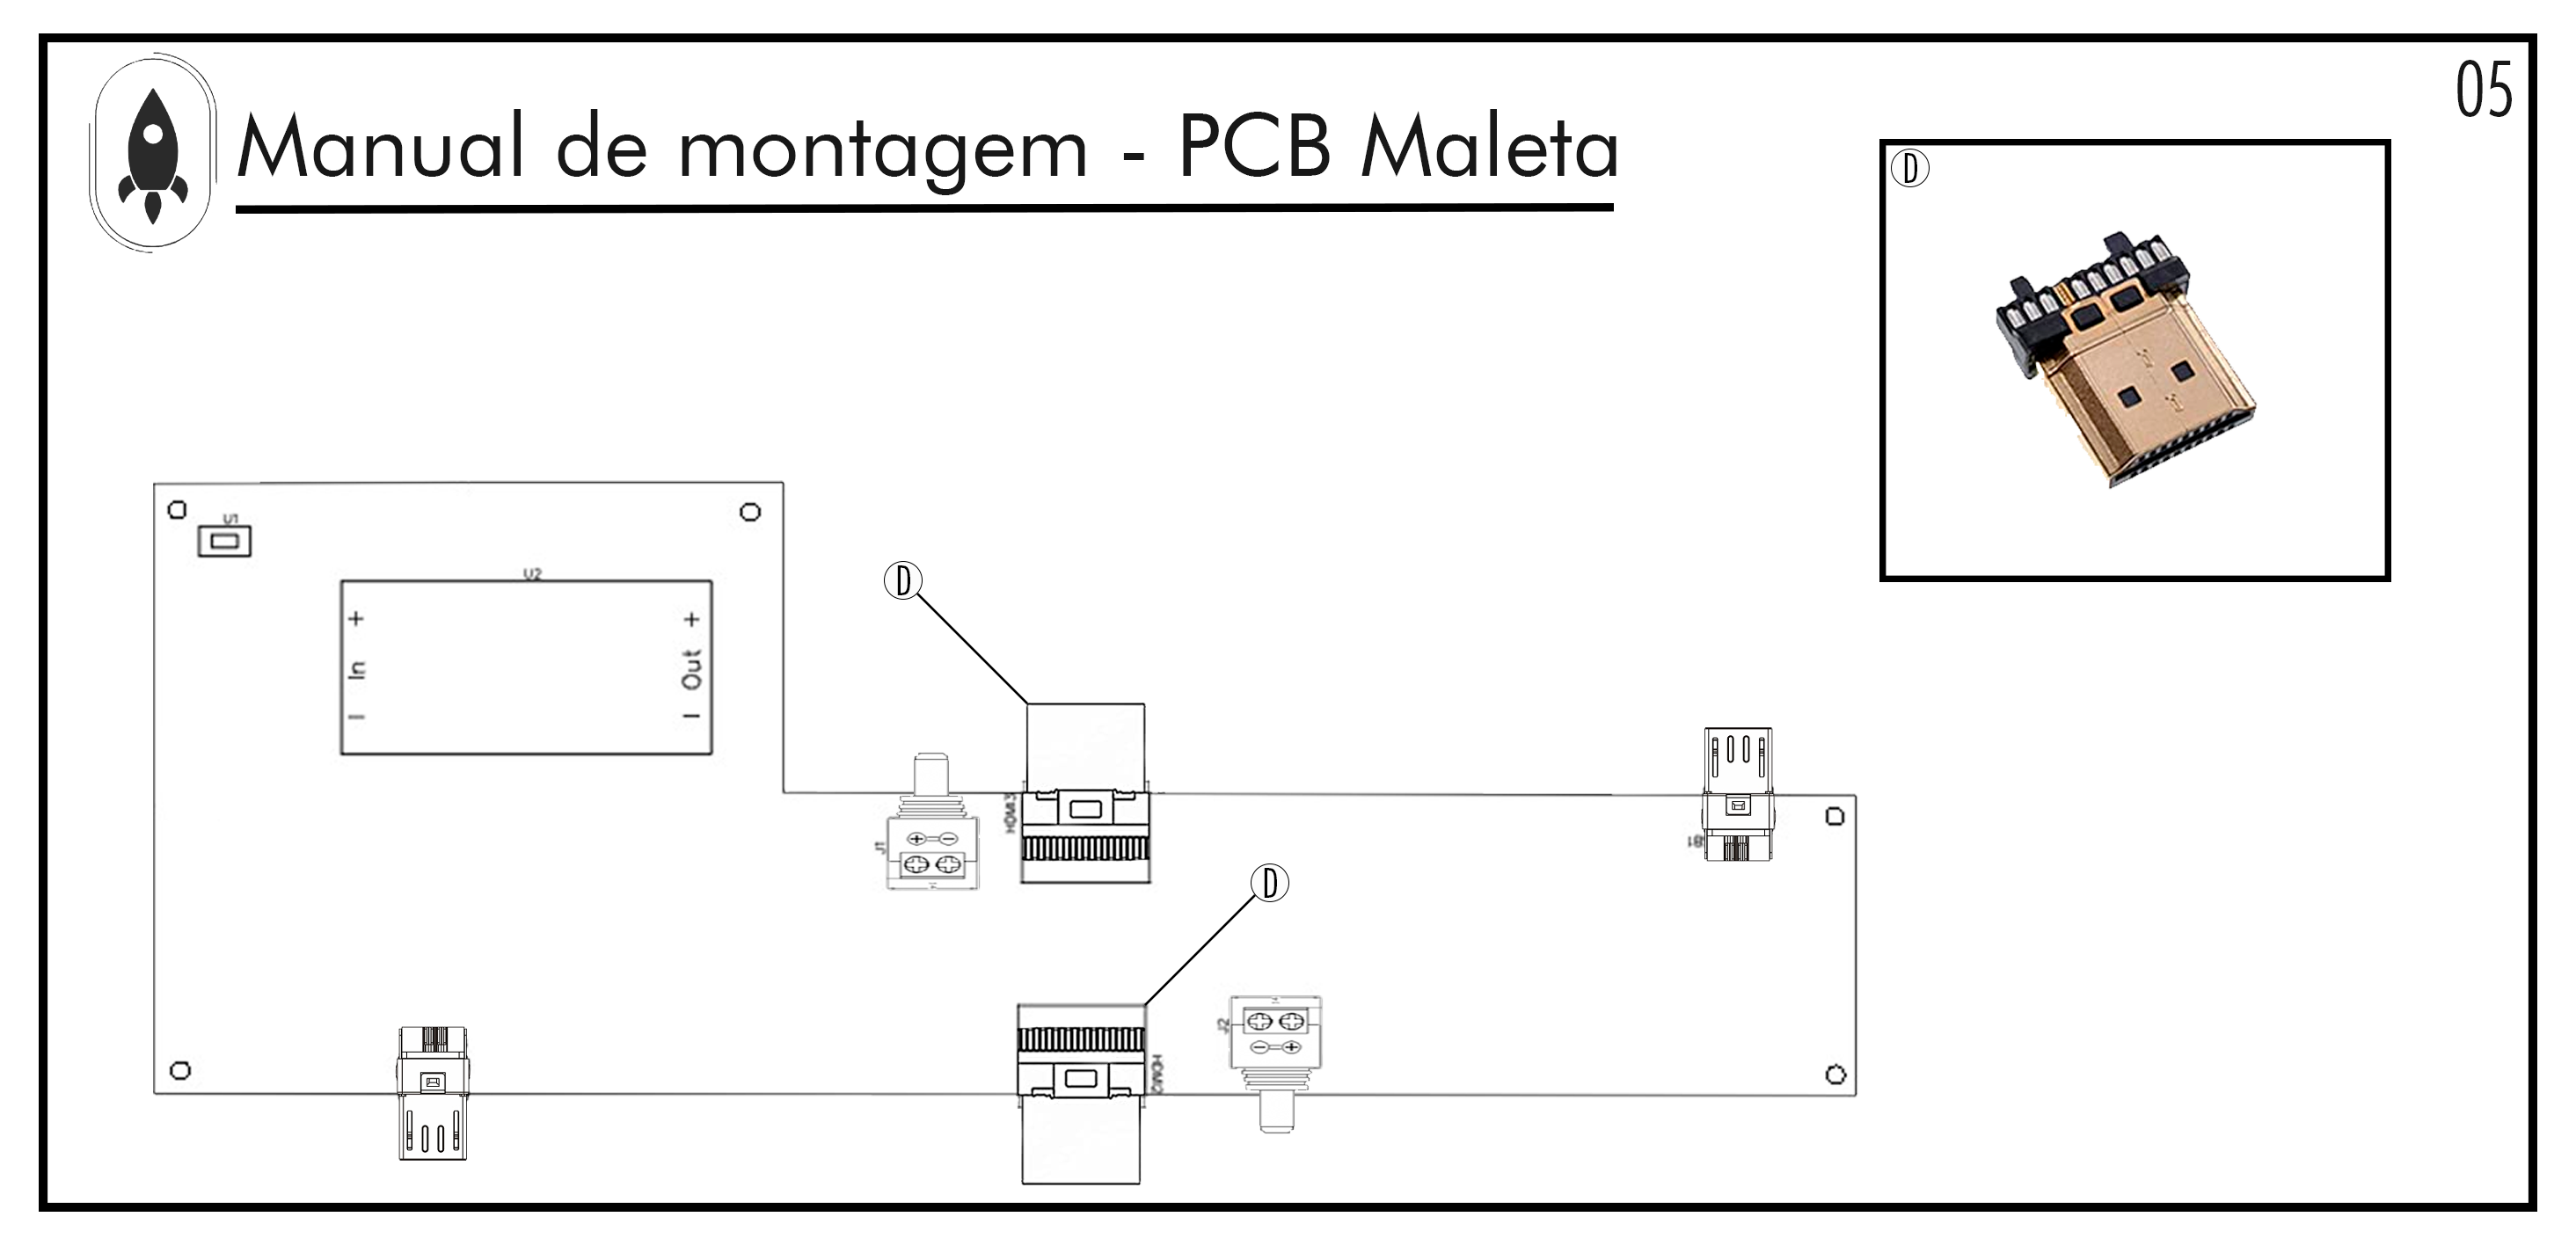
\includegraphics[width=\textwidth]{Figuras/MALETA/Pg-05---PL-01.png}
  \caption{Plug Hdmi Macho.}
 %{ \footnotesize Fonte: Autores} 
  \label{fig:PCBMALETA Hdmi}
\end{figure}


\par Pegue o componente 'E'(Conector fêmea Jack P4 2,5mm), encaixe-a na posição mostrada \ref{fig:PCBMALETA Jack} e solde junto a placa.

\begin{figure}[H]
  \centering
  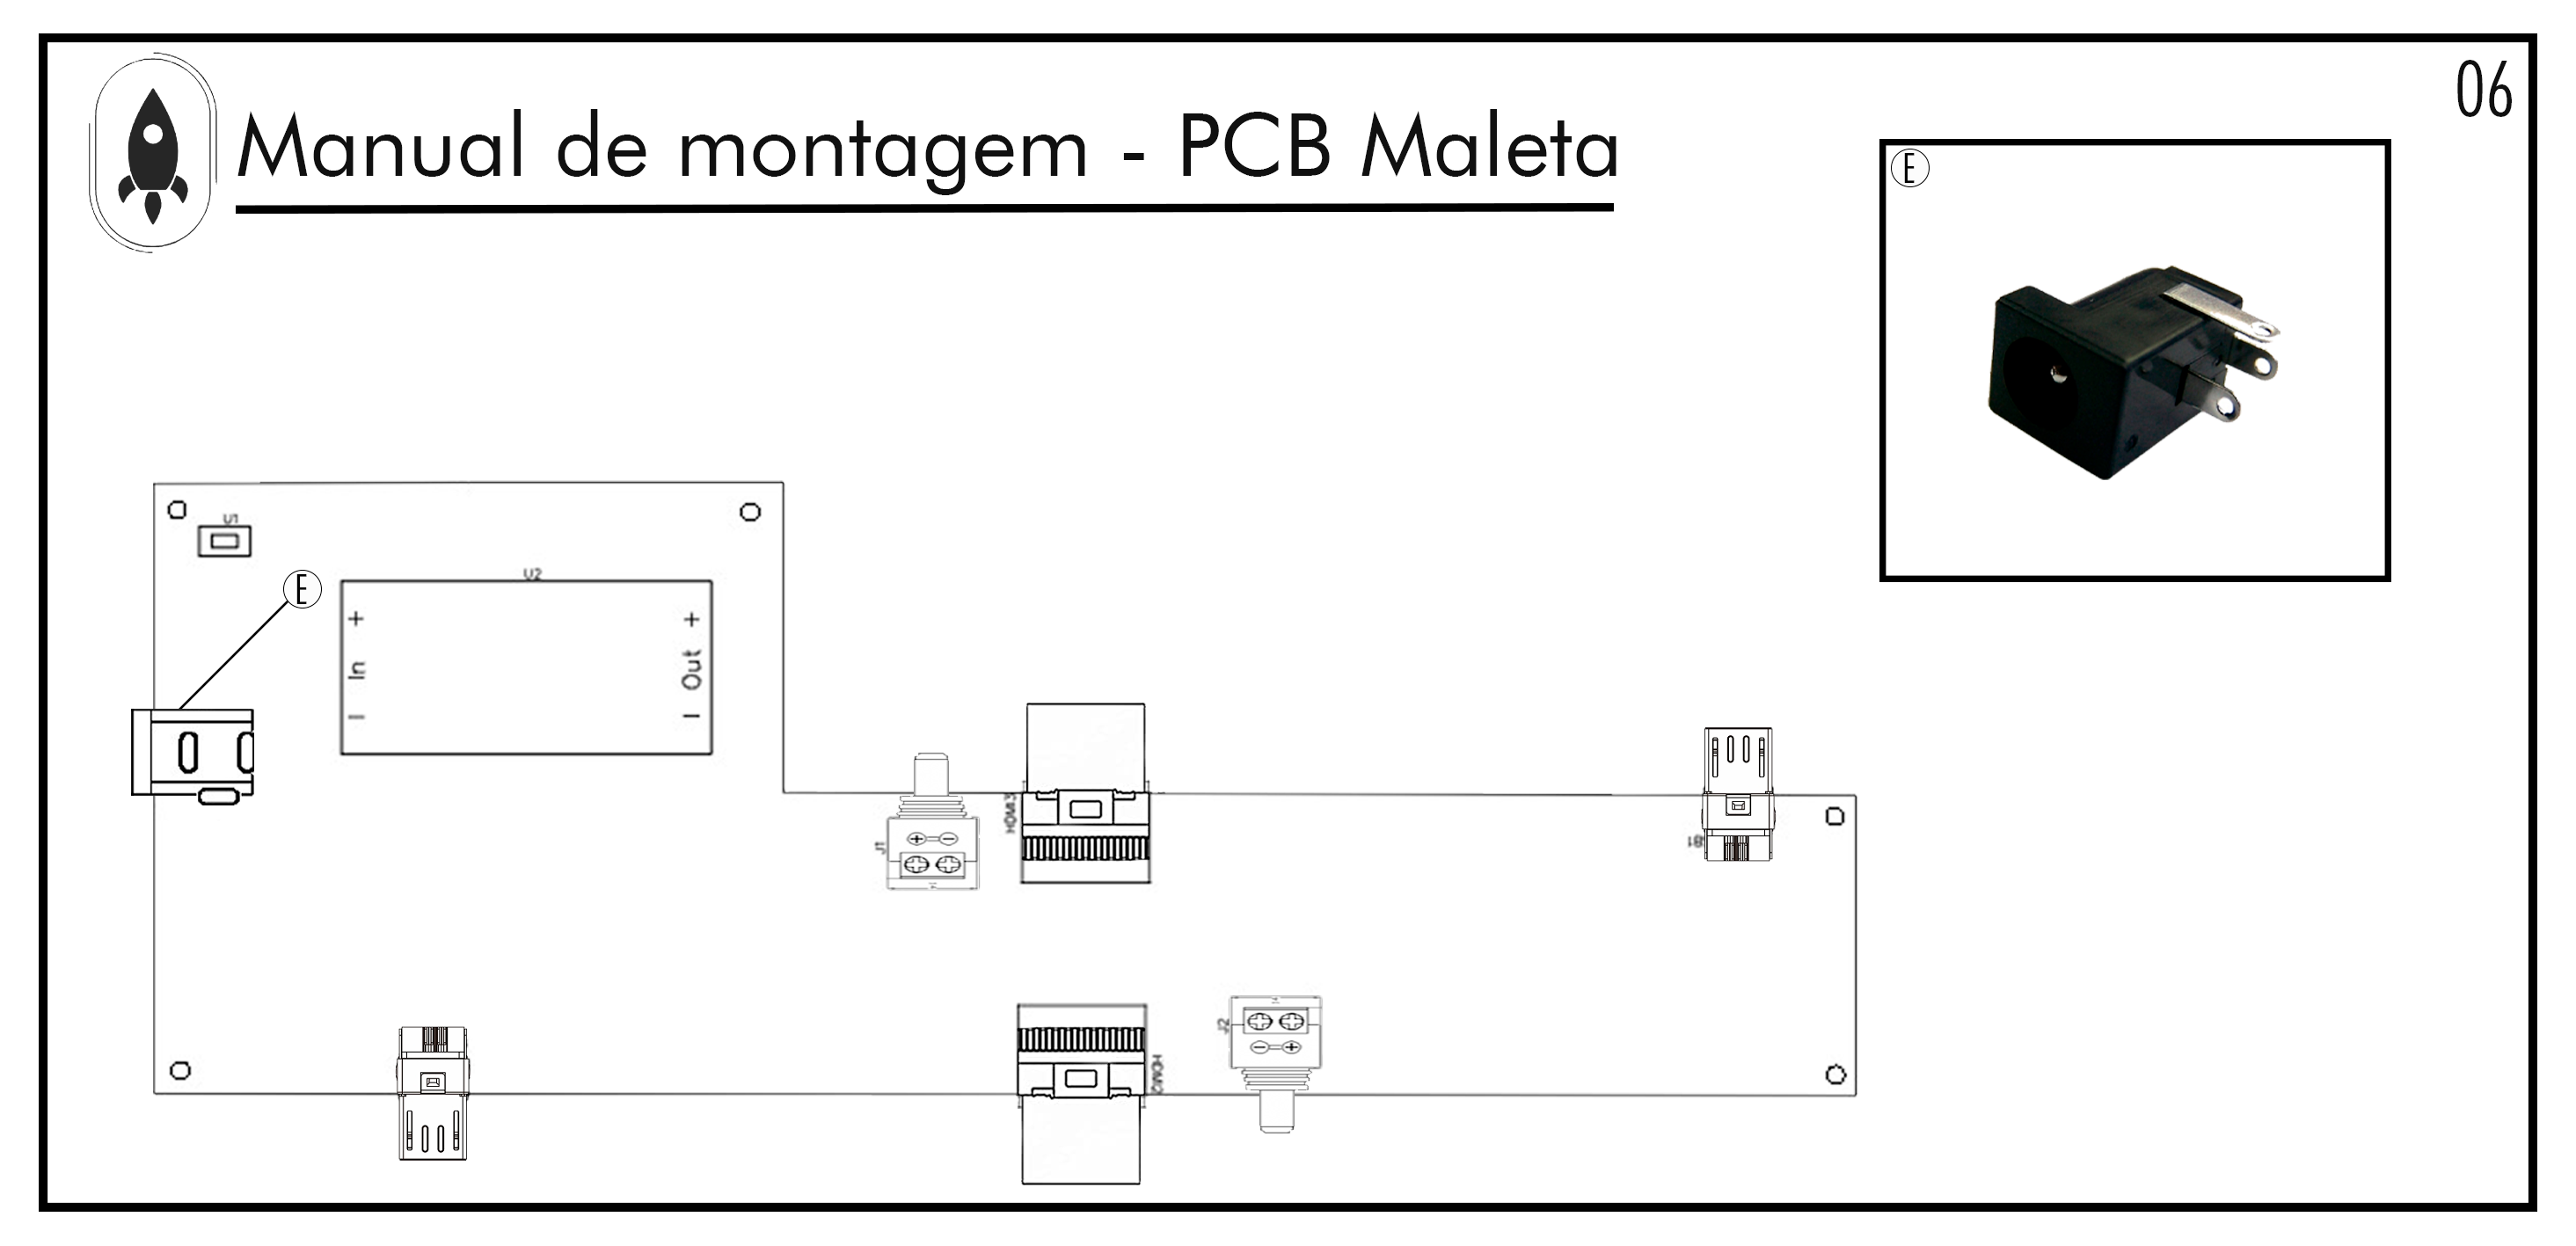
\includegraphics[width=\textwidth]{Figuras/MALETA/Pg-06---PL-01.png}
  \caption{Conector fêmea Jack P4 2,5mm.}
 %{ \footnotesize Fonte: Autores} 
  \label{fig:PCBMALETA Jack}
\end{figure}

\newpage

\par Pegue o componente 'F'(Chave Gangorra 2 Polos Mini), encaixe-a na posição mostrada \ref{fig:PCBMALETA CHAVE} e solde junto a placa.

\begin{figure}[H]
  \centering
  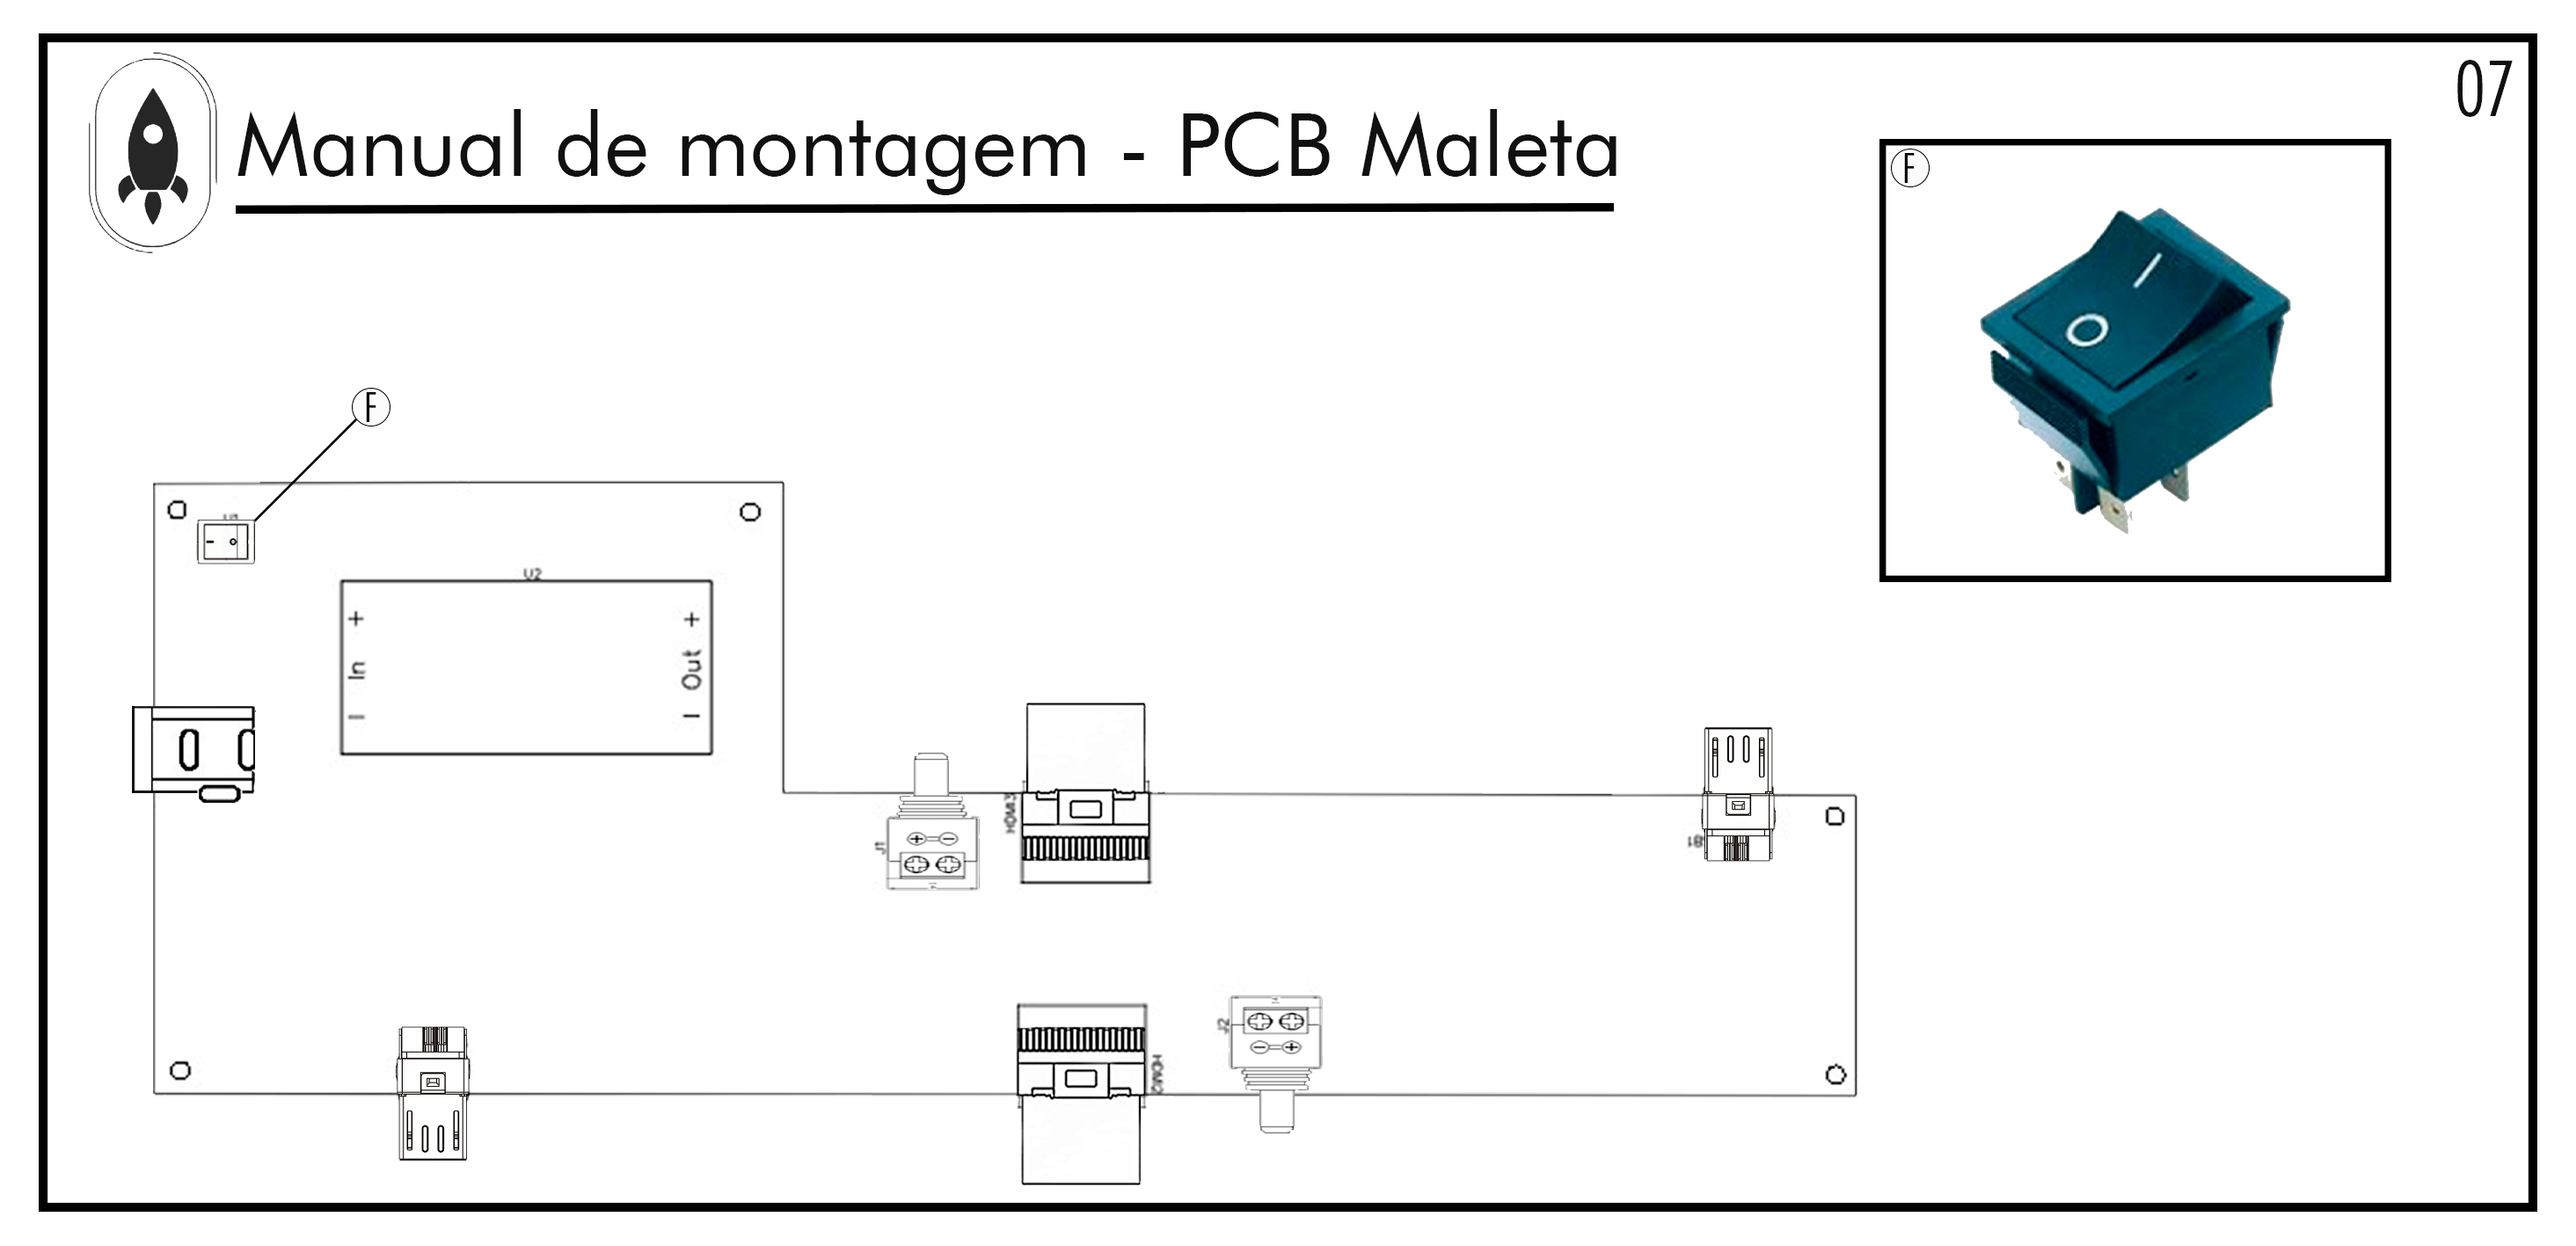
\includegraphics[width=\textwidth]{Figuras/MALETA/Pg-07---PL-01.png}
  \caption{Chave Gangorra 2 Polos Mini.}
 %{ \footnotesize Fonte: Autores} 
  \label{fig:PCBMALETA CHAVE}
\end{figure}

\par Pegue o componente 'G'(ESP32 LoRa WiFi), encaixe-a na posição mostrada \ref{fig:PCBMALETA LORA}

\begin{figure}[H]
  \centering
  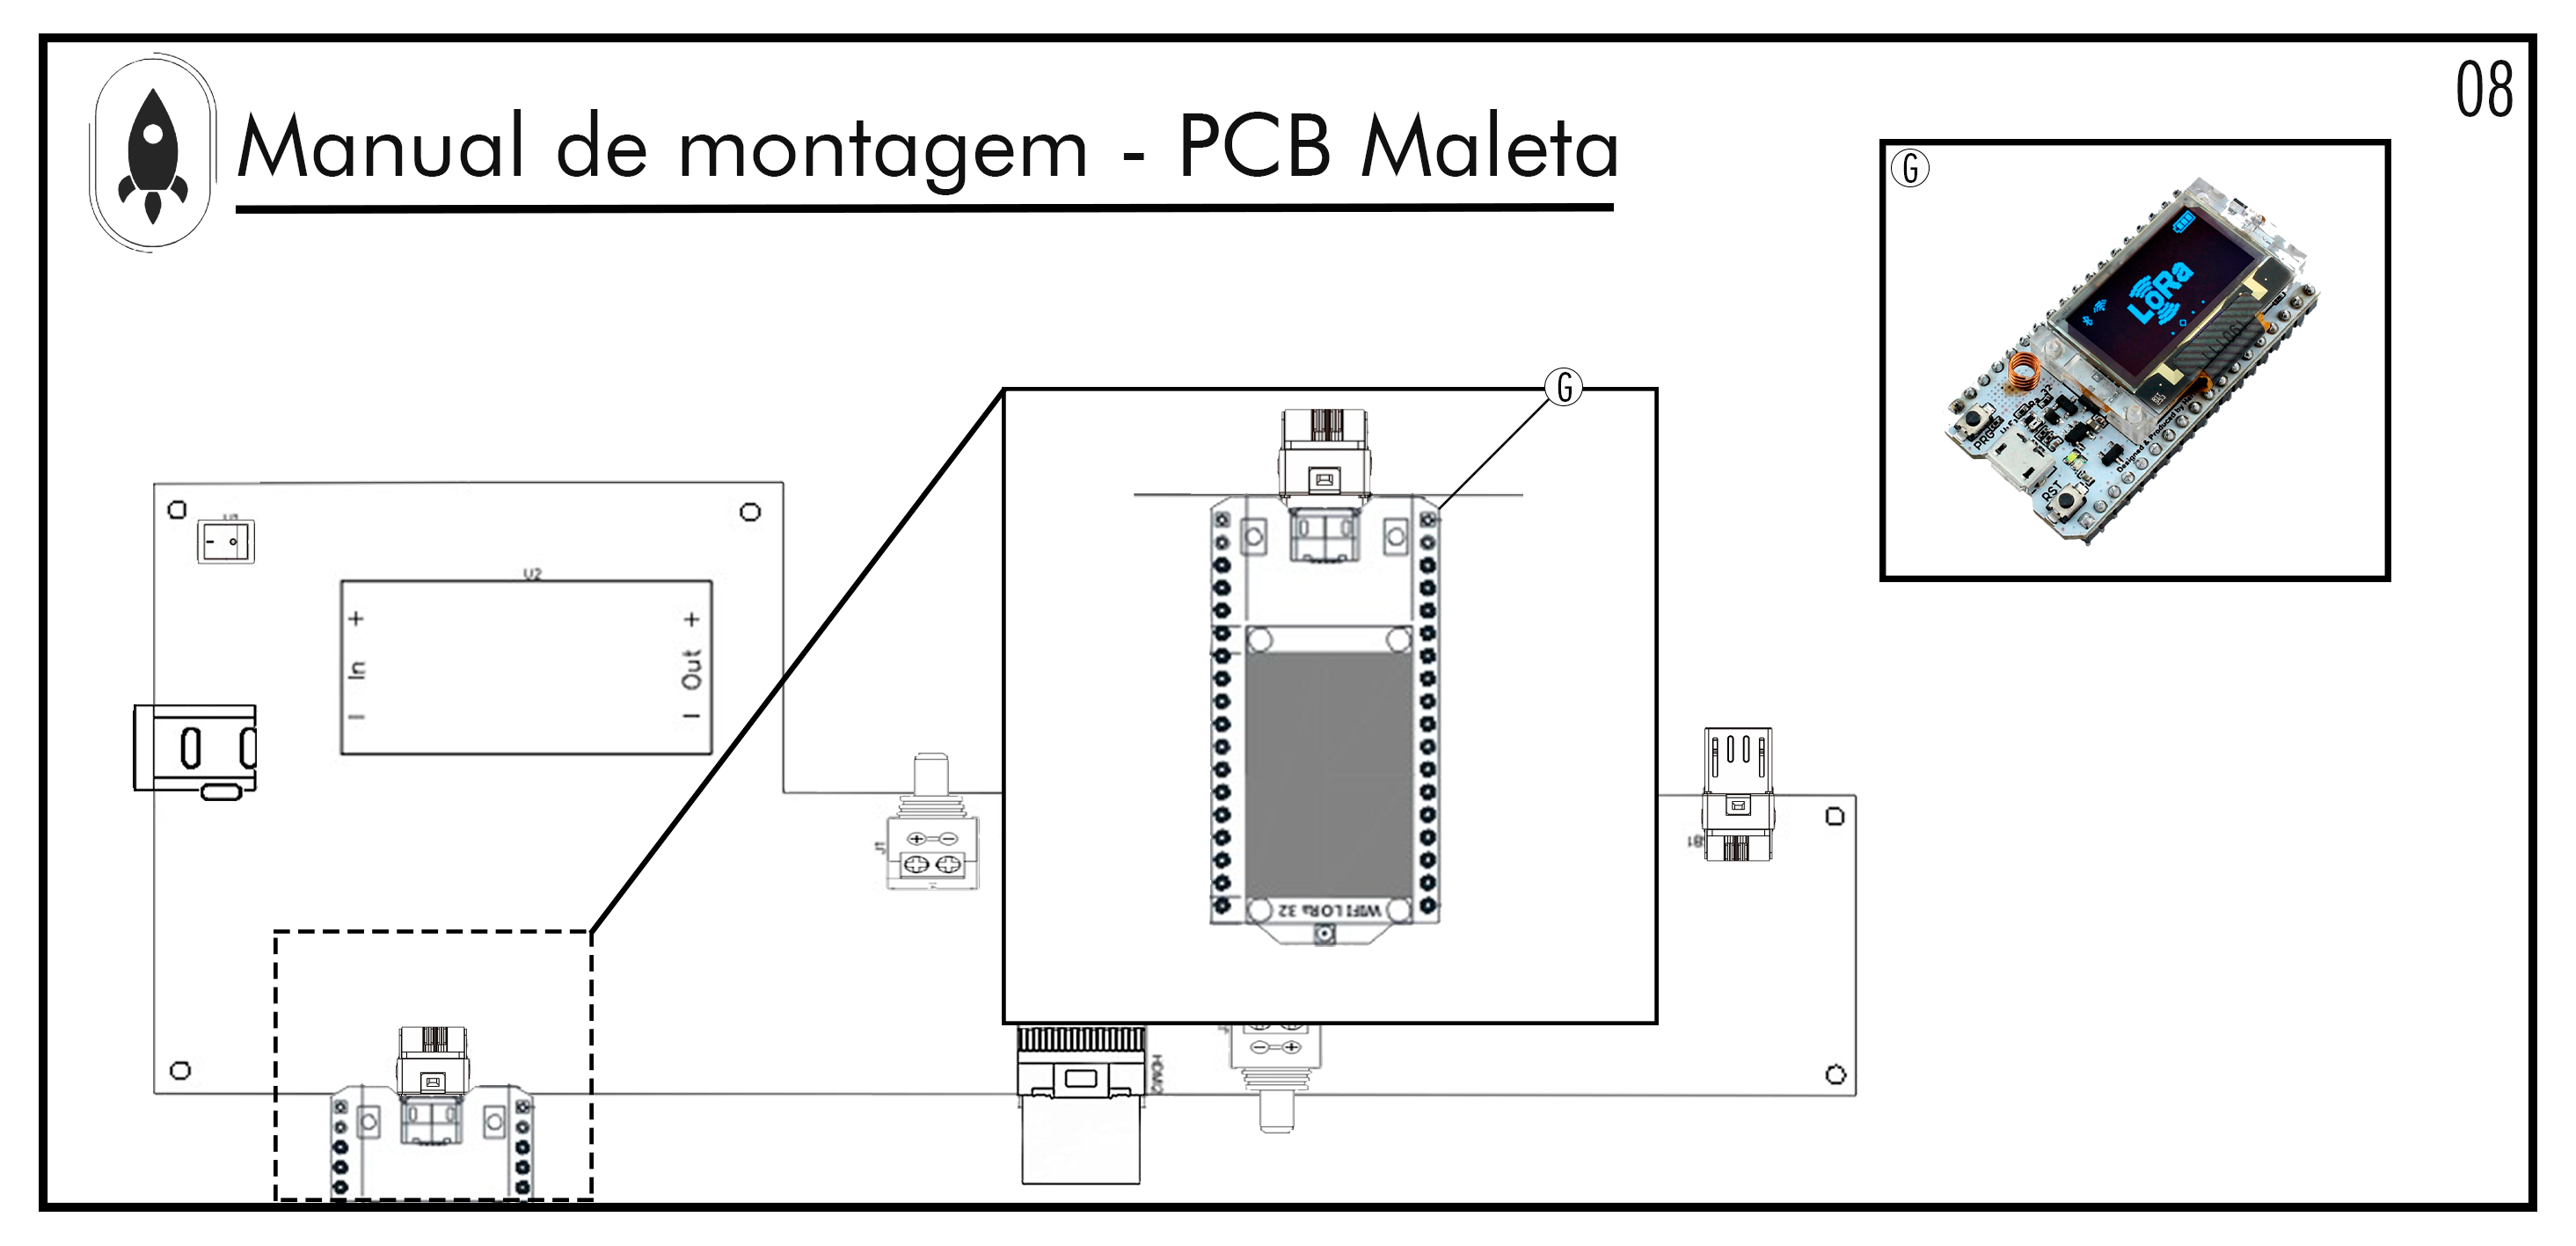
\includegraphics[width=\textwidth]{Figuras/MALETA/Pg-08---PL-01.png}
  \caption{ESP32 LoRa WiFi.}
 %{ \footnotesize Fonte: Autores} 
  \label{fig:PCBMALETA LORA}
\end{figure}
\newpage
\par Pegue o componente 'H'(NVIDIA Jetson Nano Developer Kit), encaixe-a na posição mostrada \ref{fig:PCBMALETA NVIDIA} 
\begin{figure}[H]
  \centering
  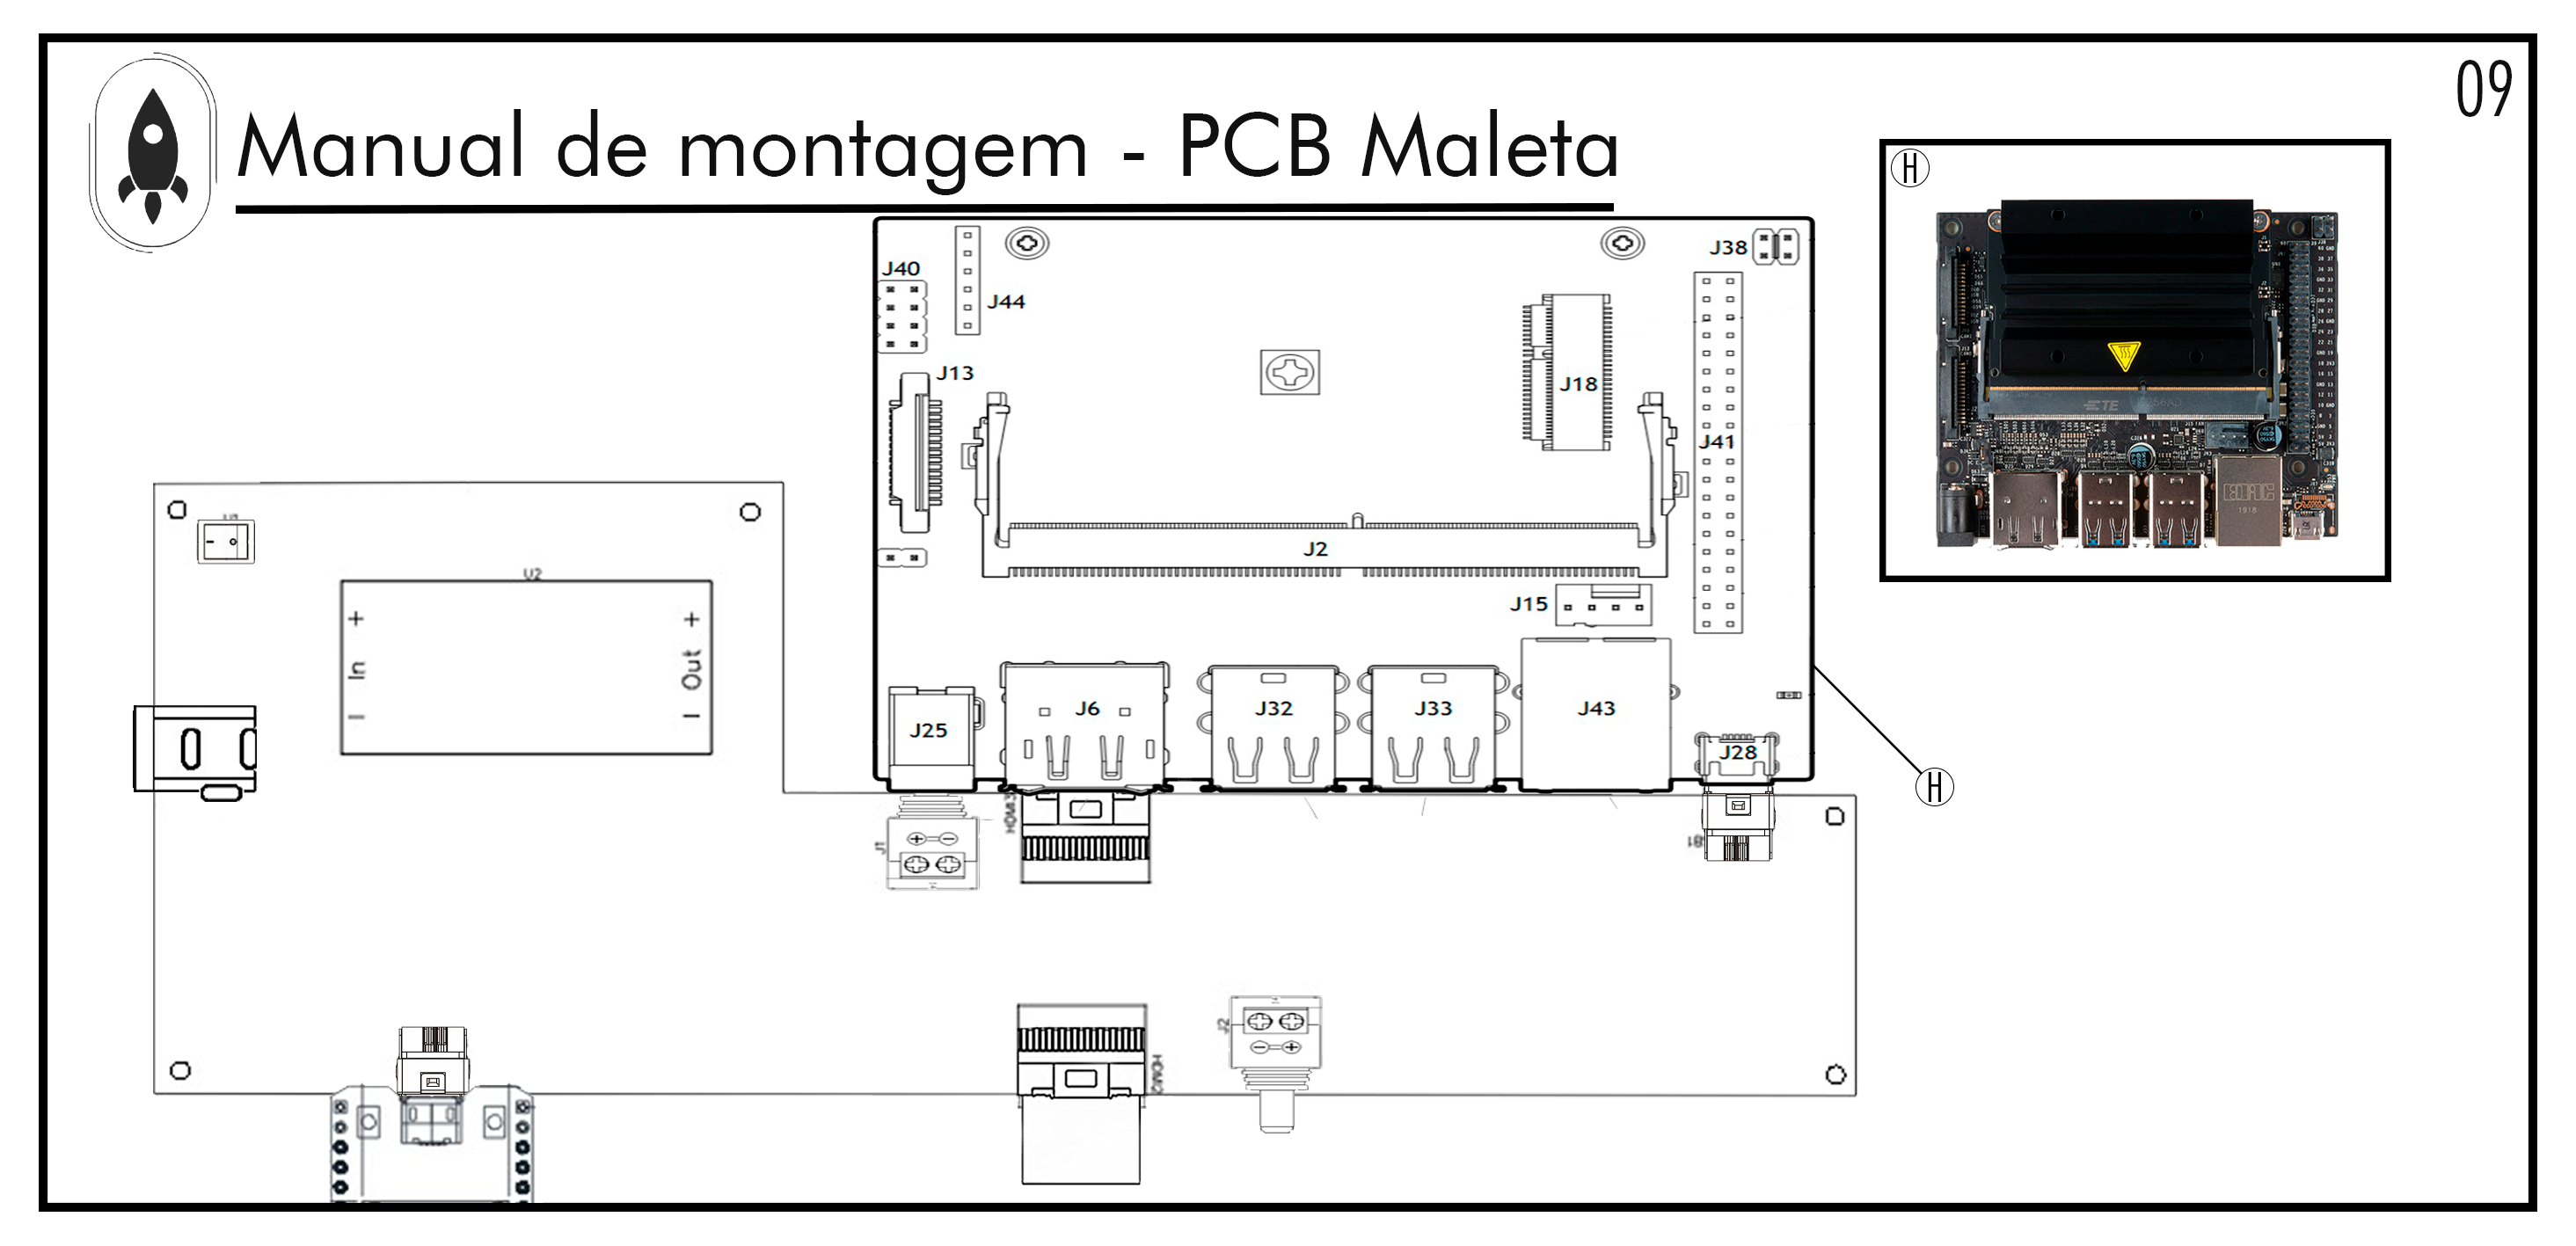
\includegraphics[width=\textwidth]{Figuras/MALETA/Pg-09---PL-01.png}
  \caption{NVIDIA Jetson Nano Developer Kit.}
 %{ \footnotesize Fonte: Autores} 
  \label{fig:PCBMALETA NVIDIA}
\end{figure}




\par Pegue o componente 'I'(Placa controladora PCB800099-V.9), encaixe-a na posição mostrada \ref{fig:PCBMALETA PCB800099} 

\begin{figure}[H]
  \centering
  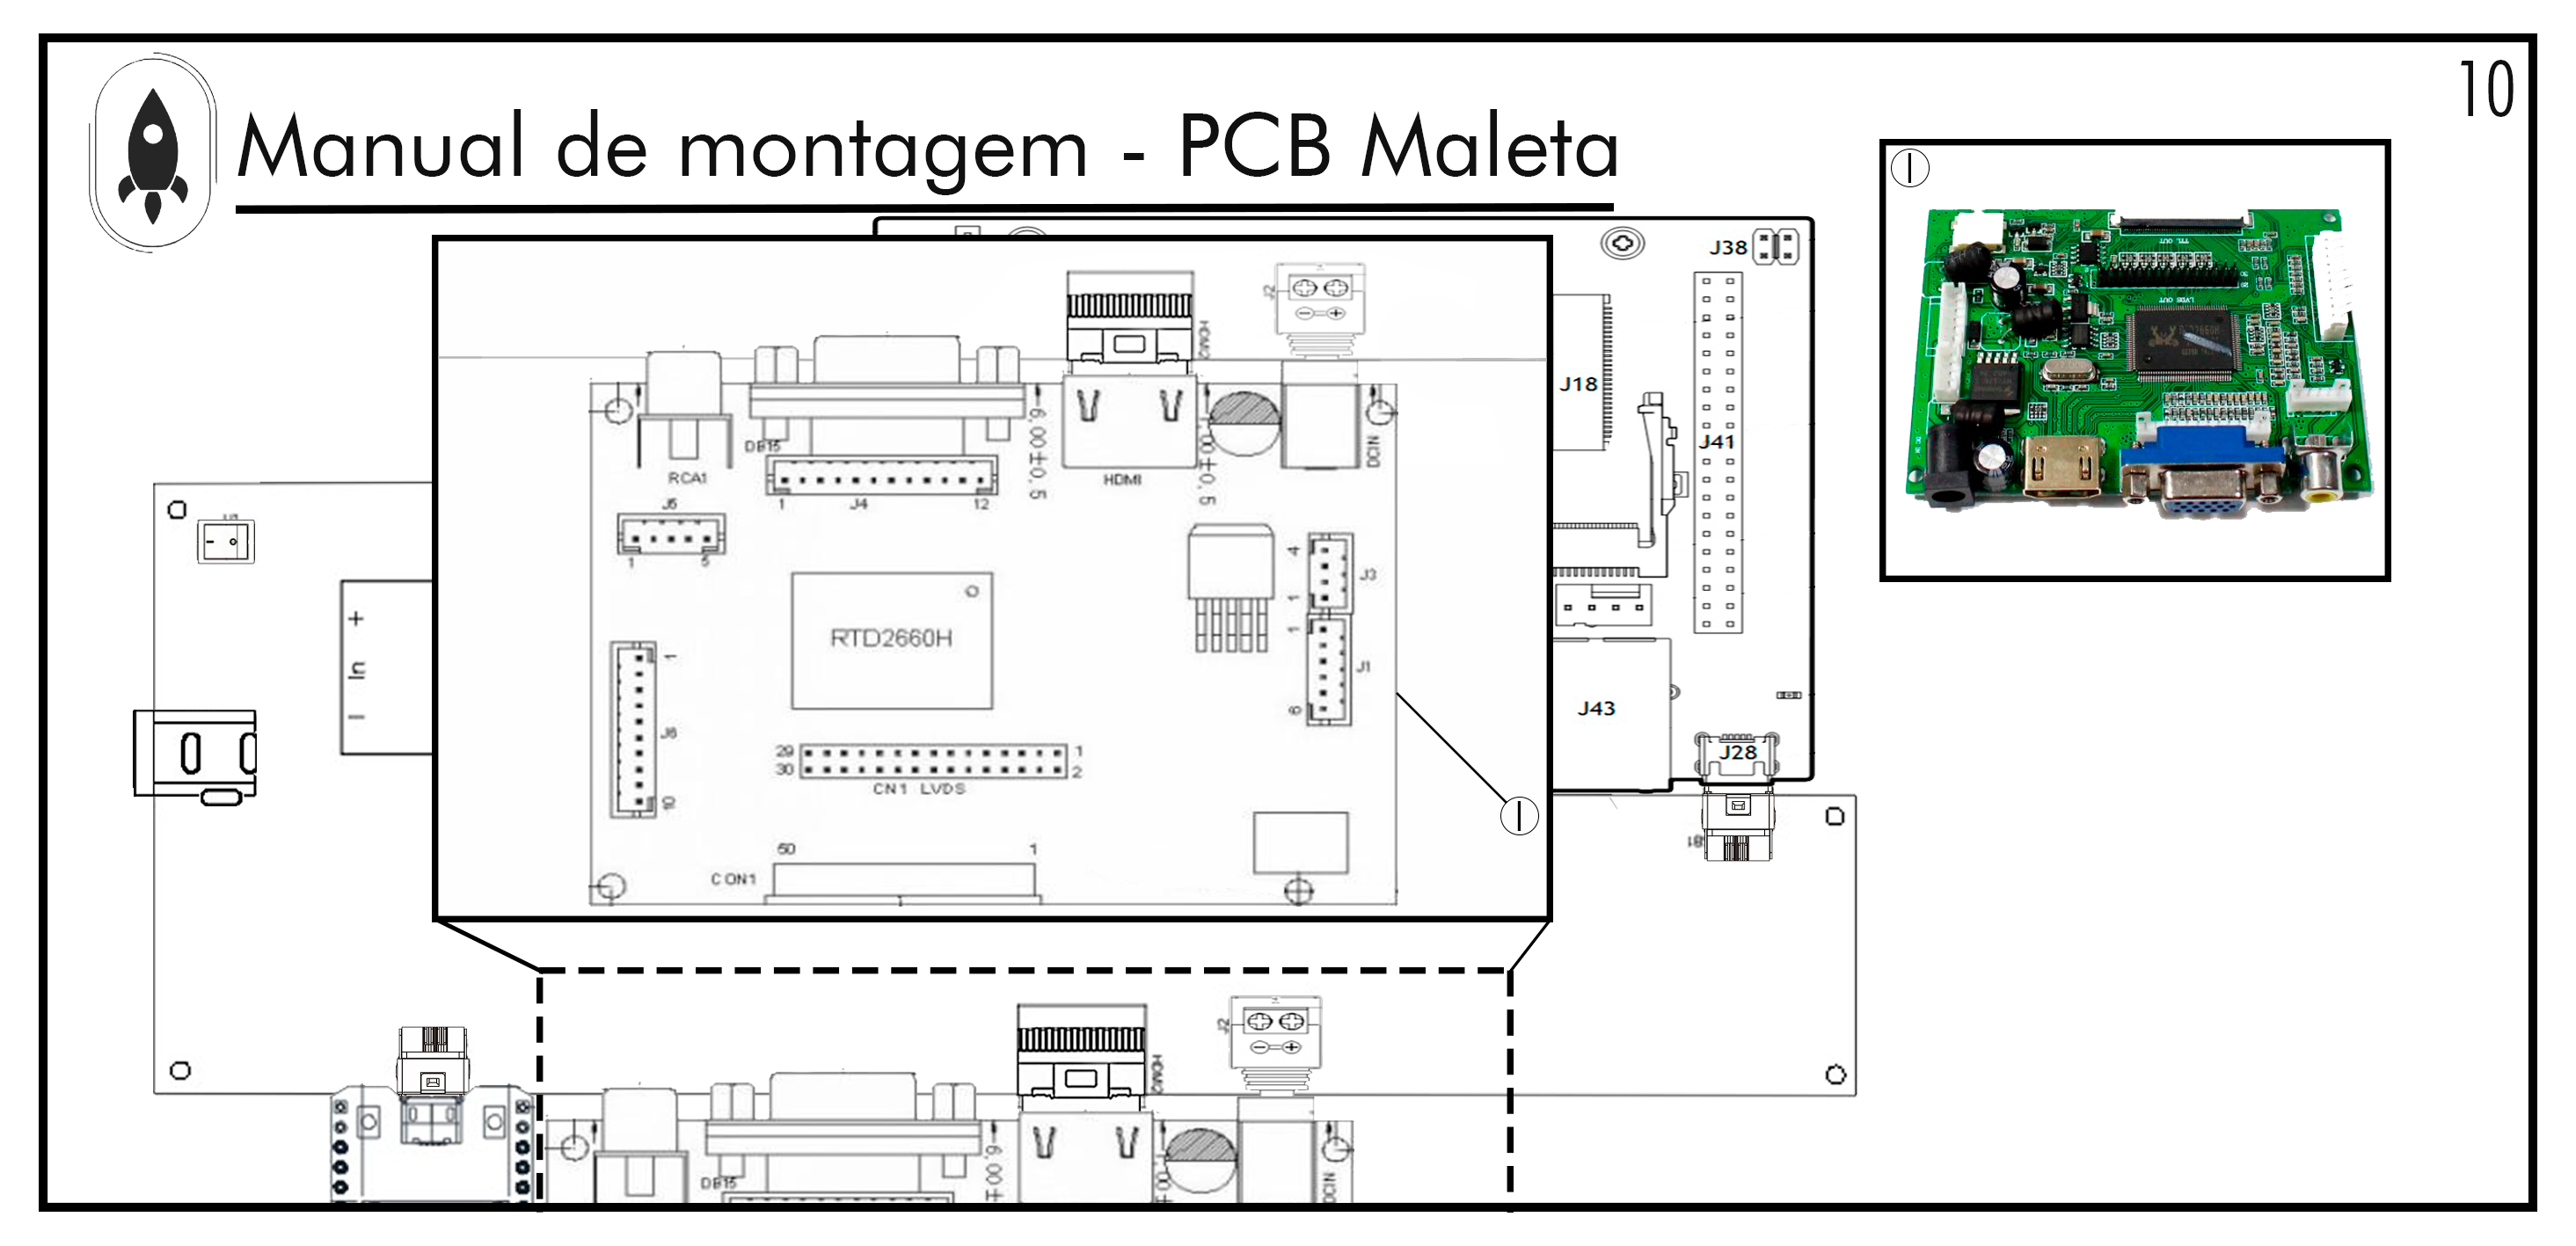
\includegraphics[width=\textwidth]{Figuras/MALETA/Pg-10---PL-01.png}
  \caption{Placa controladora PCB800099-V.9.}
 %{ \footnotesize Fonte: Autores} 
  \label{fig:PCBMALETA PCB800099}
\end{figure}

\newpage
\par Pegue o componente 'J'(LM2596), encaixe-a na posição mostrada \ref{fig:PCBMALETA LM2596} e solde junto a placa.
\begin{figure}[H]
  \centering
  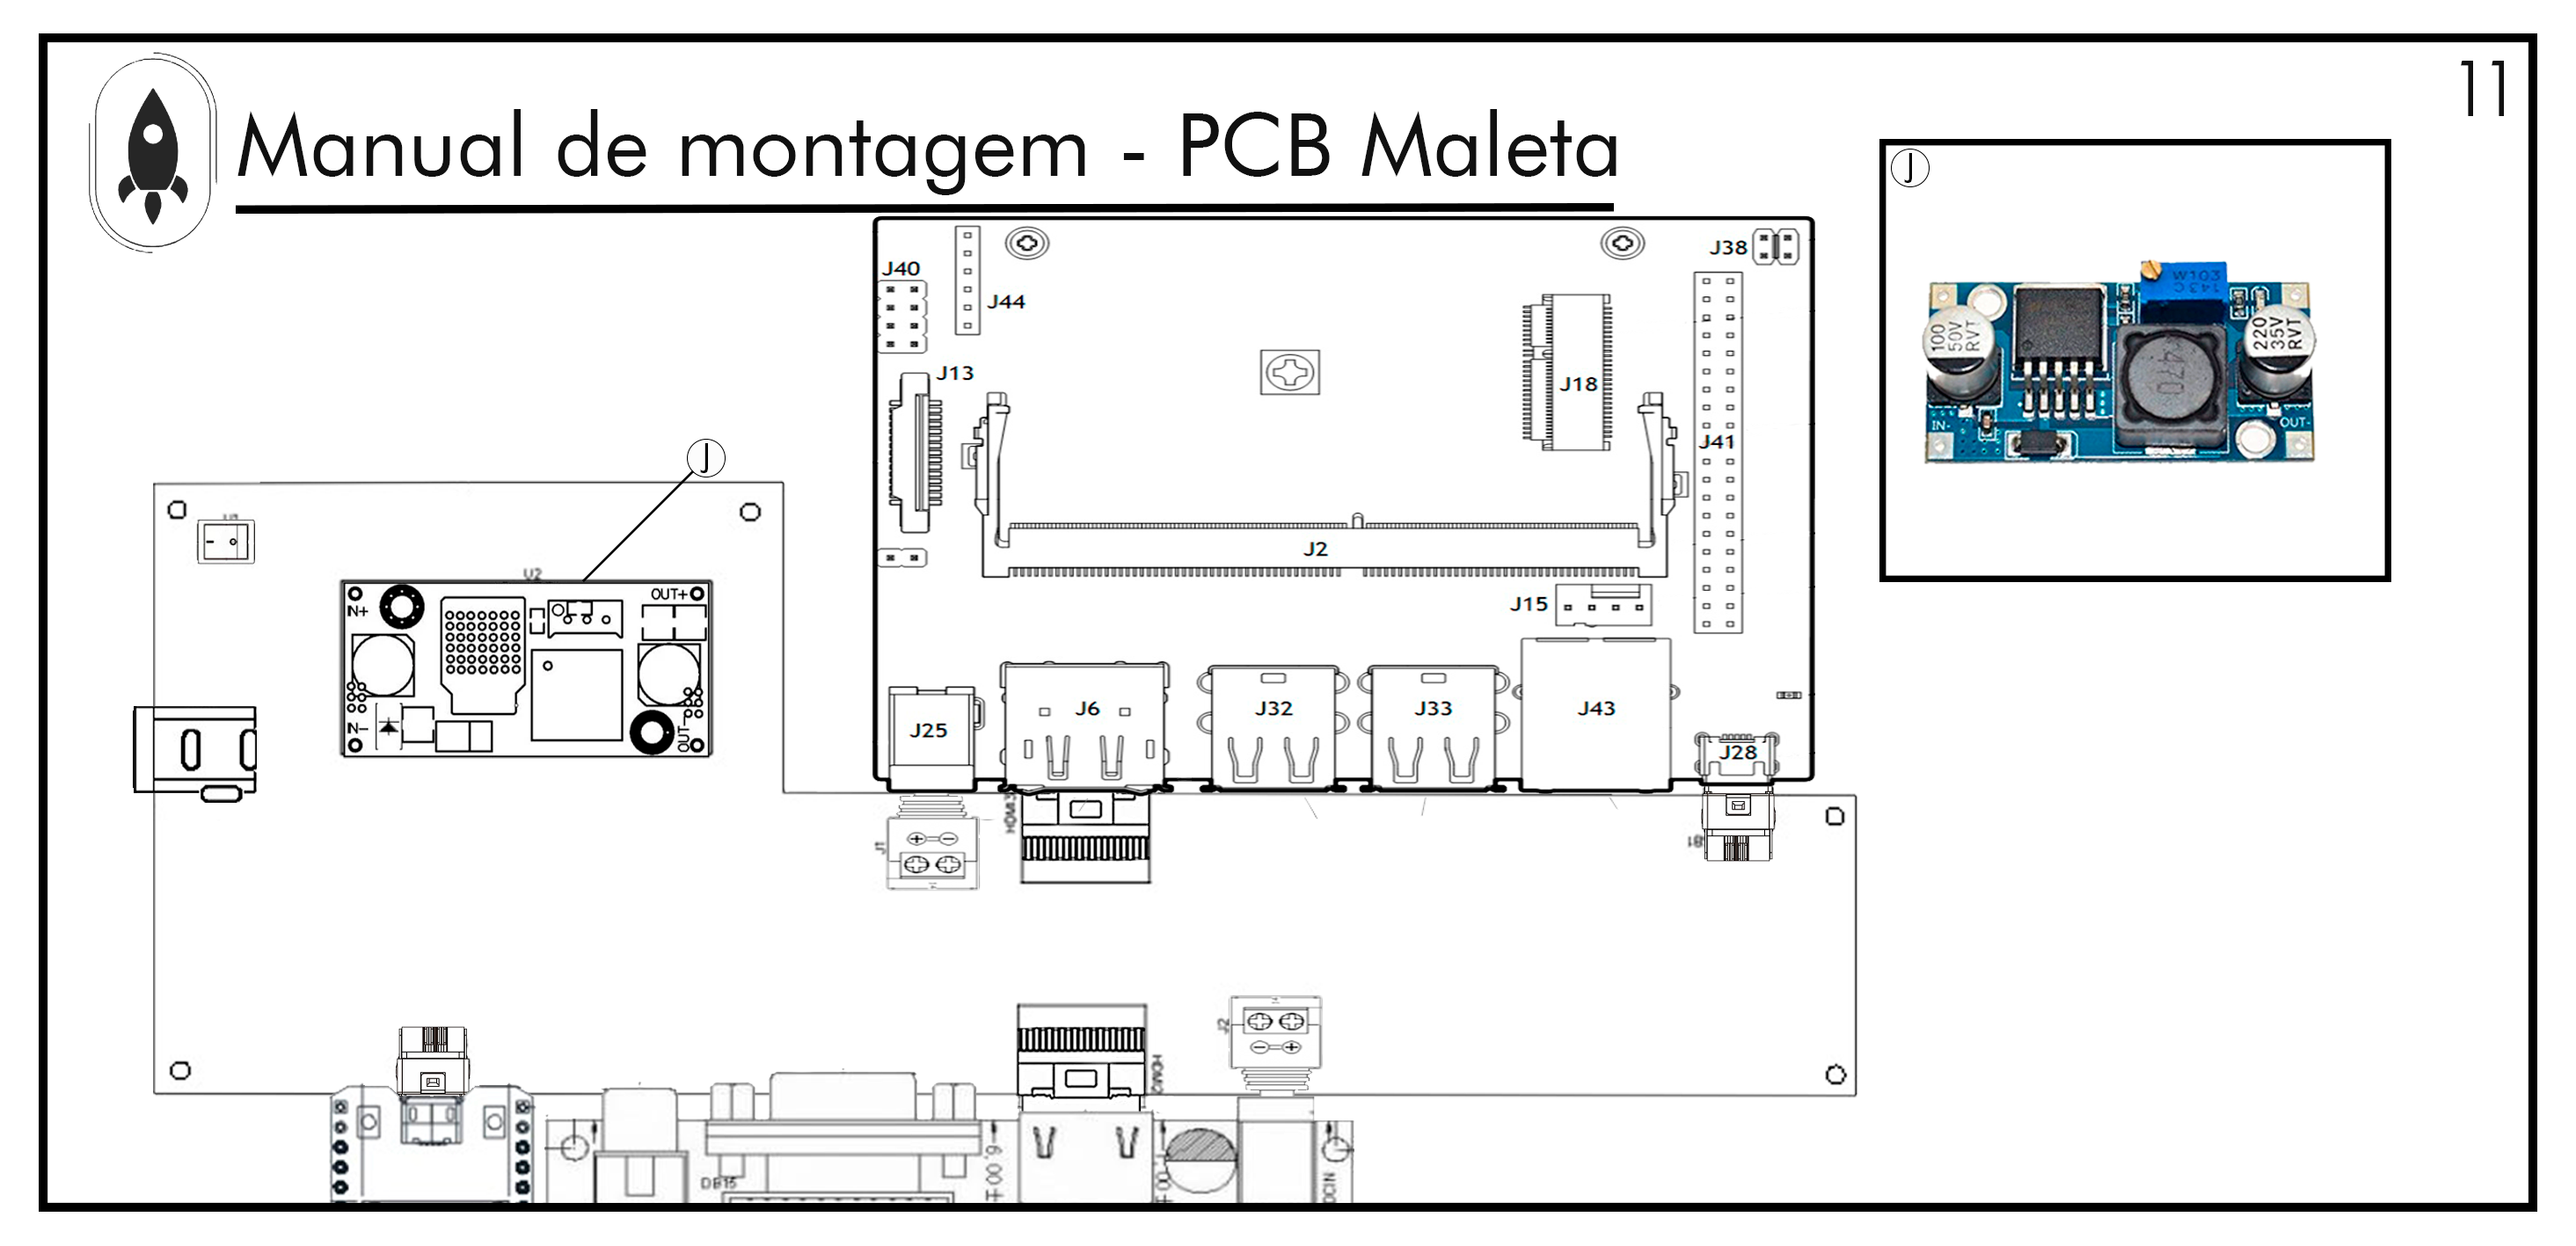
\includegraphics[width=\textwidth]{Figuras/MALETA/Pg-11---PL-01.png}
  \caption{LM2596.}
 %{ \footnotesize Fonte: Autores} 
  \label{fig:PCBMALETA LM2596}
\end{figure}



\par Pegue o componente 'K'(Display LCD 9 polegadas), encaixe-a o cabo de 50 pinos na posição mostrada \ref{fig:PCBMALETA display}.

\begin{figure}[H]
  \centering
  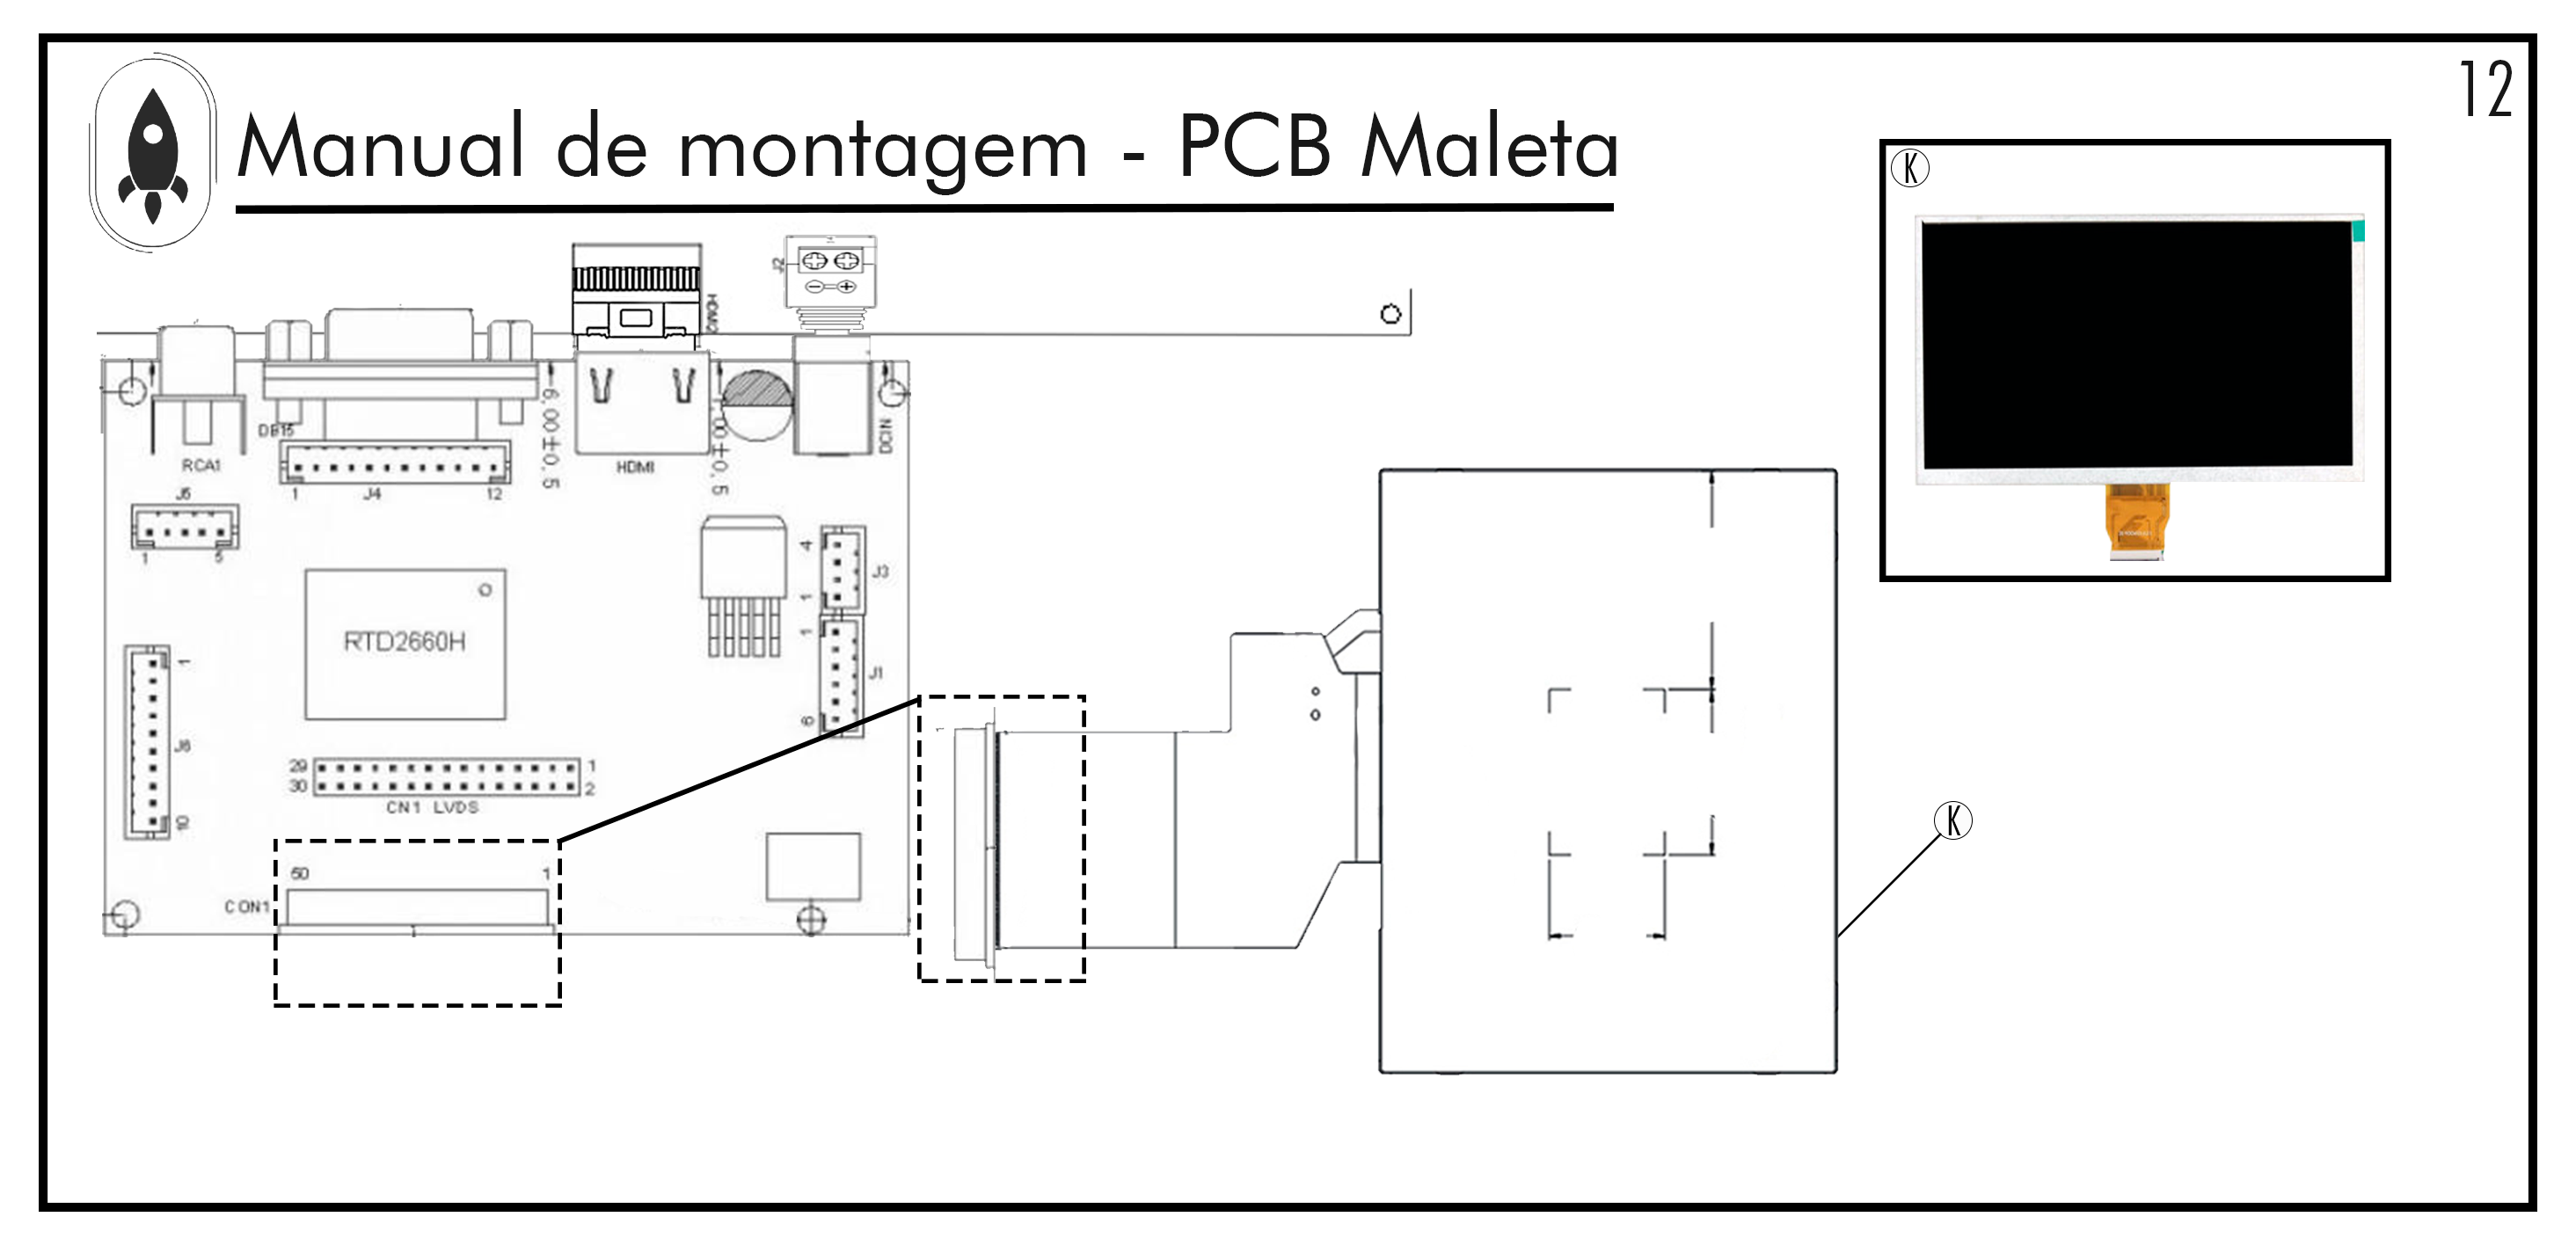
\includegraphics[width=\textwidth]{Figuras/MALETA/Pg-12---PL-01.png}
  \caption{Display LCD 9 polegadas.}
 %{ \footnotesize Fonte: Autores} 
  \label{fig:PCBMALETA display}
\end{figure}
\newpage
\par Pegue o componente 'L'(Mini Teclado slim com Touchpad), encaixe-a na posição mostrada \ref{fig:PCBMALETA Teclado} através de um cabo usb.
\begin{figure}[H]
  \centering
  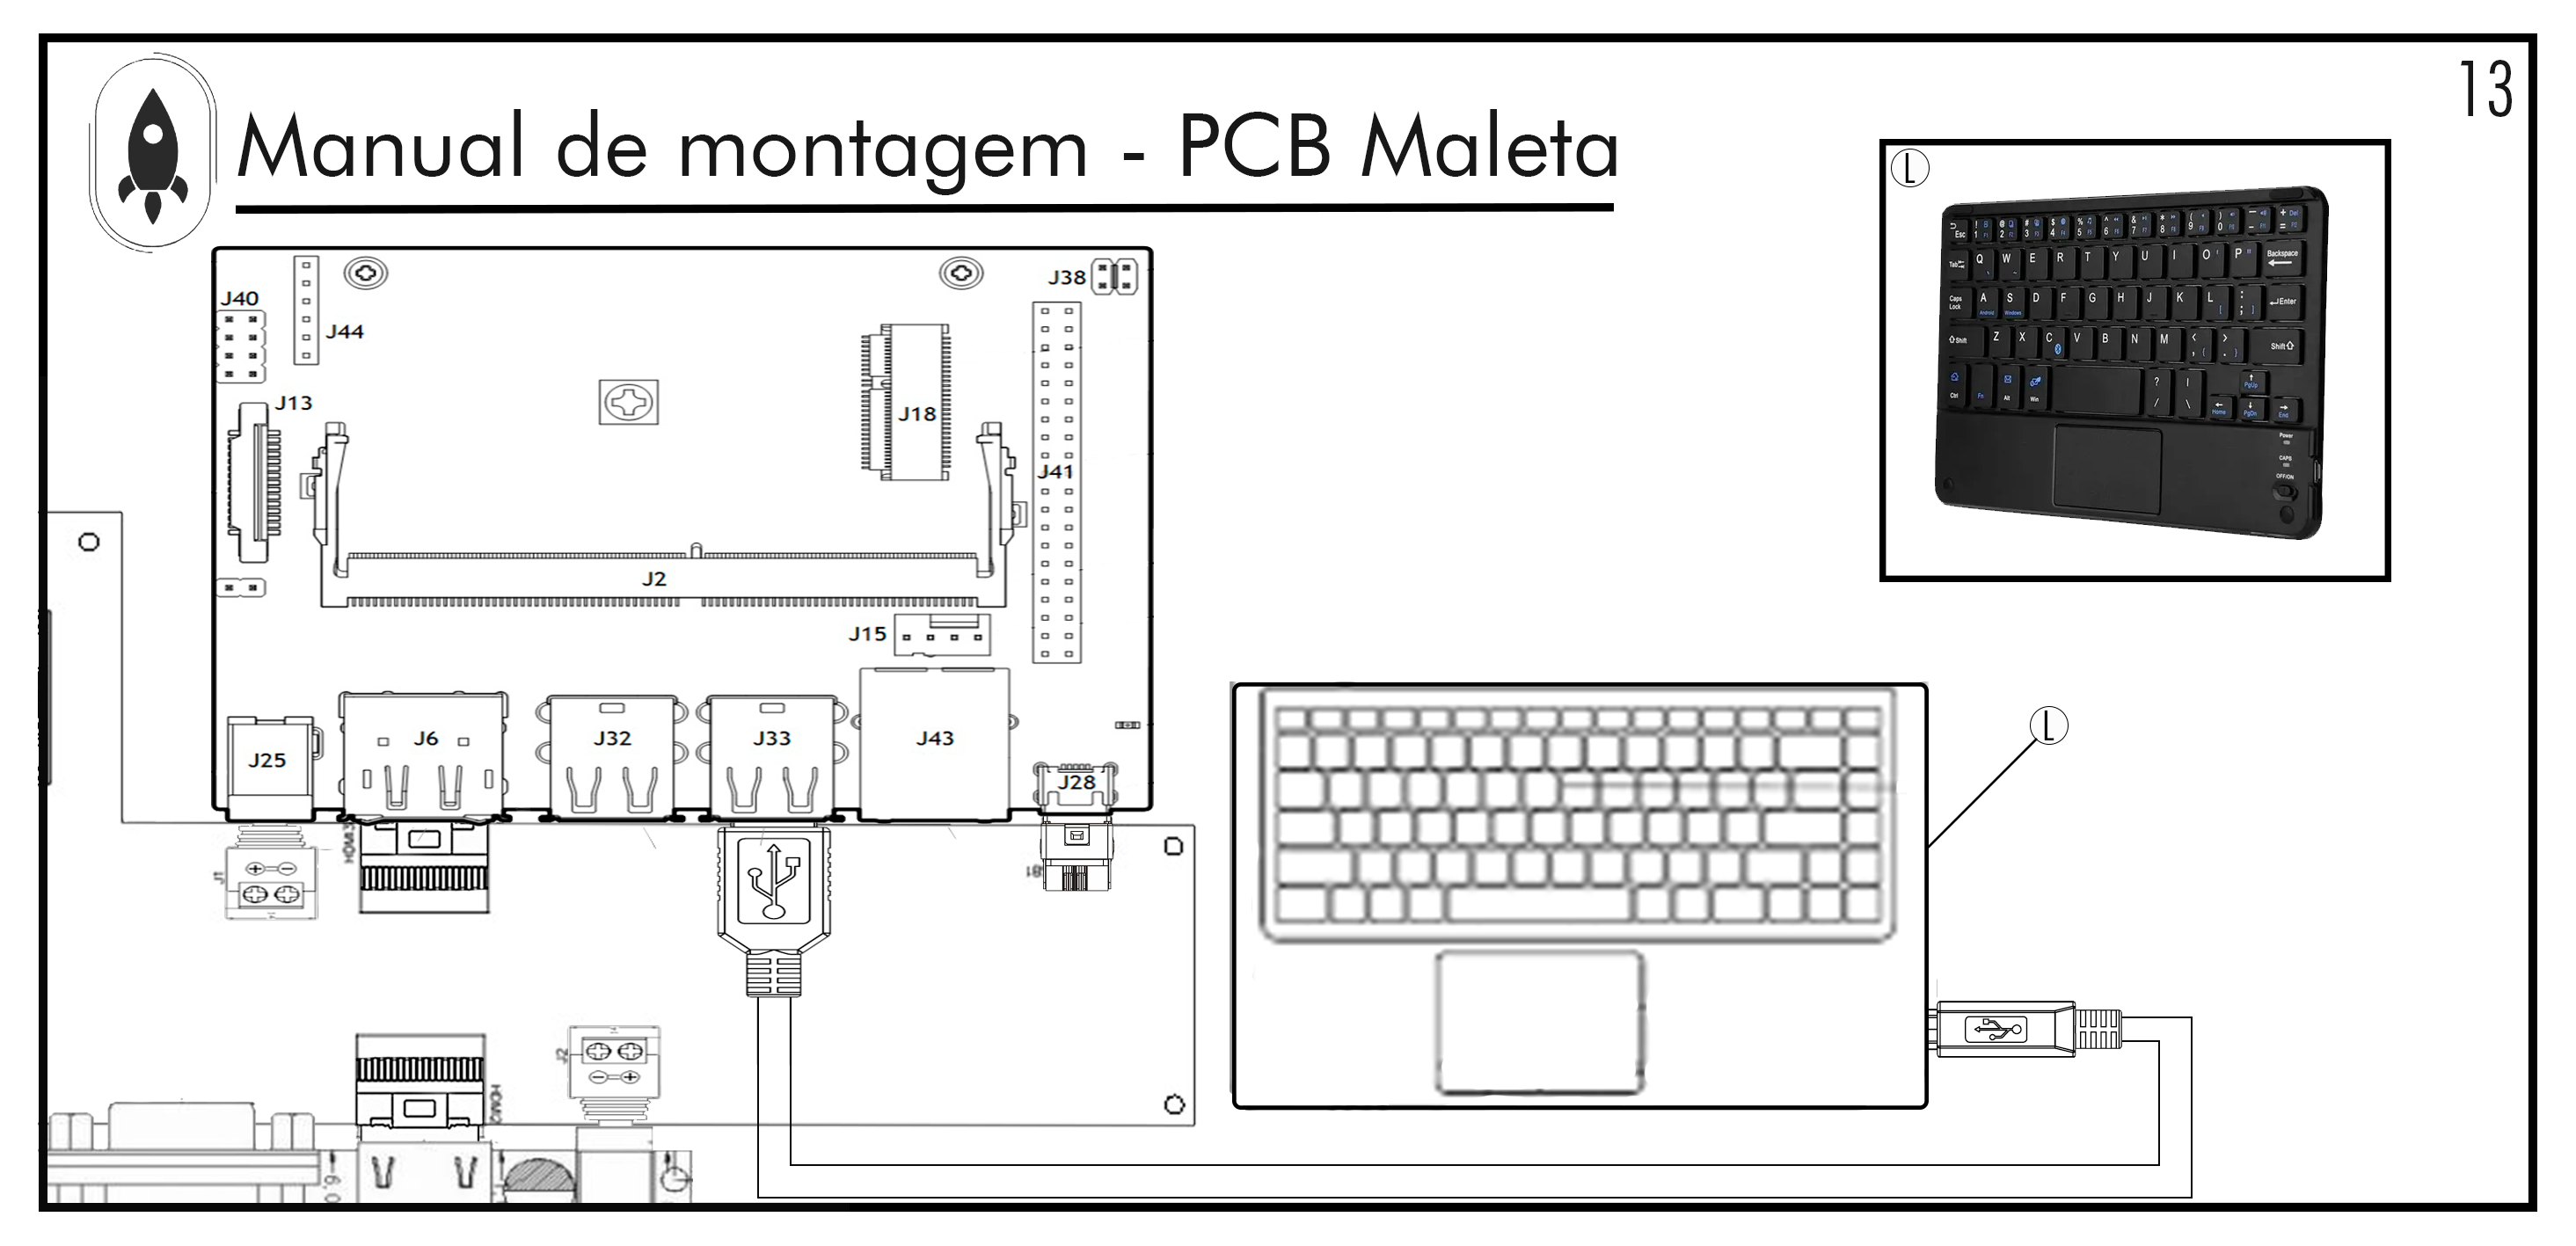
\includegraphics[width=\textwidth]{Figuras/MALETA/Pg-13---PL-01.png}
  \caption{Mini Teclado slim com Touchpad.}
 %{ \footnotesize Fonte: Autores} 
  \label{fig:PCBMALETA Teclado}
\end{figure}


\subsection{Fixação das PCI's} \label{sec:fixação  }
\par Para a correta fixação das placas de circuito impresso nos seus respectivos lugares é necessário a utilização dos parafusos e porcas extensoras de modo a garantir a fixação adequada e a integridade dos componentes.
\begin{itemize}
    \item 1-Pegue a porca extensora, posicione-a sobre o local do parafuso,
     \item 2-Pegue a placa, posicione-a sobre o porca extensora,
     \item 3-Pegue o parafuso, posicione-a sobre o local de colocar o parafuso da placa,
    \item 4-Com ajuda de uma chave philips parafuse-o sem apertar de mais para evitar problemas mecânicos a placa,
    \item 5-Repita o processo para outros parafusos.
     
\end{itemize}

\begin{figure}[H]
  \centering
  \includegraphics[scale=0.1]{Figuras/100pcs-lot-10-brass-standoffs-m3-hex-nut.jpg}
    \includegraphics[scale=0.3]{Figuras/parafuso.png}
  \caption{Parafuso e porca extensora M5.}
  \label{fig:parafusos}
\end{figure}

\subsection{Case de proteção PCI's da Base de Lançamento}
\par Para acomodar e proteger a placa responsável pelo hardware na base de lançamento foi feita uma case de proteção conforme mostrada na figura \ref{fig:Case de proteção da PCI vistas} nela sera acomodada a PCI e alguns conectores para organizar as saídas.
\begin{figure}[H]
  \centering
  \includegraphics[scale=0.4]{Figuras/BASE/case f.png}

  \caption{Case de proteção da PCI saídas.}
  \label{fig:Case de proteção da PCI saídas}
\end{figure}
\begin{figure}[H]
  \centering
 % \includegraphics[scale=0.7]{Figuras/BASE/case iso.png}
  \includegraphics[scale=0.5]{Figuras/BASE/Sem título.png}
    \includegraphics[scale=0.7]{Figuras/BASE/case.png}
  \caption{Case de proteção da PCI vistas.}
  \label{fig:Case de proteção da PCI vistas}
\end{figure}
\PAR Os fios que alimentaram os motores e as células de cargas vão sair dos reles acoplados na PCI para conectores P4 acoplados a case de proteção para facilitar o encaixe dos fios até os atuadores como mostrado na figura \ref{fig:Case de proteção da PCI render}, são cabos Antichama Flexível 450/750 V de seção nominal 0,75mm².

\begin{figure}[H]
  \centering
  \includegraphics[scale=0.2]{Figuras/BASE/untitled.11.jpg}
  \includegraphics[scale=0.2]{Figuras/BASE/untitled.12.jpg}
  \caption{Case de proteção da PCI.}
  \label{fig:Case de proteção da PCI render}
\end{figure}